\documentclass[11pt]{book}
\usepackage[utf8]{inputenc}
\usepackage[T1]{fontenc}
\usepackage[margin=1.3in]{geometry}

%For Baskerville if wanted
\usepackage{kpfonts,baskervald}
\usepackage[multiple]{footmisc}
\usepackage{cancel}
\usepackage{float}
\usepackage{comment}
\usepackage{mathtools}
\usepackage{etoolbox}

%Bib style
\bibliographystyle{jhep}
\usepackage{cite}

%For better equations and such.
\usepackage{amsmath}
\usepackage{stmaryrd}
\usepackage{physics}

%For tables.
\usepackage[table,xcdraw]{xcolor}
\usepackage{enumitem}
\usepackage{slashed}
\usepackage{multirow}

%For better quivers
\usepackage[all]{xy}

%For tikz and plots
\usepackage{adjustbox}
\usepackage{tikz}
\usetikzlibrary{positioning,
				cd,
				decorations.markings, 
				arrows.meta,
				tqft,
				calc}
\usepackage{pgfplots}
\usepackage[labelfont=bf]{caption}
\usepackage{blindtext}
\pgfplotsset{compat=1.17} 

\usepackage{tcolorbox}
\tcbuselibrary{theorems}
\newtcbtheorem[number within=section]{defn}{Definition}%
{colback=green!5,colframe=green!35!black,fonttitle=\bfseries}{df}
\newtcbtheorem[number within=section]{thm}{Theorem}%
{colback=green!5,colframe=red!35!black,fonttitle=\bfseries}{th}
\newtcbtheorem[number within=section]{Jargon}{Jargon}%
{colback=green!5,colframe=blue!35!black,fonttitle=\bfseries}{jr}
%For numbered lemmas, theorems etc.
\usepackage{amsthm}
\theoremstyle{definition}
\newtheorem{example}{Example}[section]
\newtheorem{proposition}{Proposition}[section]
\newtheorem{corollary}{Corollary}[section]
\newtheorem{conjecture}{Conjecture}[section]
\newtheorem{rem}{Remark}
\newtheorem{claim}{Claim}

%For unnumbered remarks.
\newtheorem*{remark}{Remark}

%For better numbering of equations.
\numberwithin{equation}{section}


%For clickable table of contents
\usepackage{hyperref}
\definecolor{airforceblue}{rgb}{0.36, 0.54, 0.66}
\hypersetup{
    colorlinks,
    citecolor=purple,
    filecolor=black,
    linkcolor=airforceblue,
    urlcolor=blue
}
\usepackage[nameinlink]{cleveref}

%%%%%%%

\newcommand{\flux}[2][]{[\rho_{#2}^{#1}]^{y_S}_{y_N}}
\NewDocumentCommand{\fluxx}{ O{} O{} m m}{[\rho_{#3}^{#1}\rho_{#4}^{#2}]^{y_S}_{y_N}}

\usepackage[bbgreekl]{mathbbol}

\usepackage{bbold}
\DeclareSymbolFontAlphabet{\mathbb}{AMSb}
\DeclareSymbolFontAlphabet{\mathbbl}{bbold}

\newcommand{\Spindle}{\mathbbl{\Sigma}}
%%%%%%%%%%%%%%%%%%%%%%%%%%%%%%%%%%%%%%%%%%%%%%%%%%%%%%%%%%%%%%%%%%%
%%%%%%%%%%%%%%%%%%%%%%%%Handy macros%%%%%%%%%%%%%%%%%%%%%%%%%%%%%%%
%%%%%%%%%%%%%%%%%%%%%%%%%%%%%%%%%%%%%%%%%%%%%%%%%%%%%%%%%%%%%%%%%%%
\renewcommand*\rm[1]{\mathrm{#1}}

%For cohomology group macros
\DeclareMathOperator{\HH}{H}
\DeclareMathOperator{\cHH}{\check{H}}
\DeclareMathOperator{\Hom}{Hom}


%For correct infinitesimals.
\newcommand*\diff{\mathop{}\!\mathrm{d}}
\newcommand*\Diff{\mathop{}\!\mathrm{D}}

%For correct imaginary unit
\newcommand*\I{\mathrm{i}}

%Letters
\usepackage{dowith}
\newcommand{\UpperCase}[1]{
  \expandafter\newcommand\csname bb#1\endcsname{\mathbb{#1}}
  \expandafter\newcommand\csname c#1\endcsname{\mathcal{#1}}
  \expandafter\newcommand\csname Fr#1\endcsname{\mathfrak{#1}}   }
\DoWith\UpperCase ABCDEFGHIJKLMNOPQRSTUVWXYZ\StopDoing

\newcommand{\LowerCase}[1]{
  \expandafter\newcommand\csname Fr#1\endcsname{\mathfrak{#1}}   }
\DoWith\LowerCase abcdefghijklmnopqrstuvwxyz\StopDoing

%Common script letters
\newcommand*\scrt{\mathscr{T}}
\newcommand{\ab}[1]{#1^{\mathrm{ab}}}
\newcommand{\GL}[1]{\mathrm{GL}(#1)}
\newcommand{\PGL}[1]{\mathrm{PGL}(#1)}
\newcommand*\U{\mathrm{U}}
\newcommand*\SU{\mathrm{SU}}
\newcommand*\SO{\mathrm{SO}}
\newcommand*\OO{\mathrm{O}}
\newcommand*\SL{\mathrm{SL}}
\newcommand*\USp{\mathrm{USp}}
\newcommand*\Alt{\mathrm{Alt}}
\newcommand*\Sym{\mathrm{Sym}}
\newcommand*\bbCt{\mathbb{C}^\times}
\newcommand*\QFT{\mathbf{QFT}}
\newcommand{\ddv}{\mathrm{d}_V}

%%%%%%%%%%%%%%%%%%%%%%%%%%%%%%%%%%%%%%%%%%%%%%%%%%%%%%%%%%%%%%%%%%%

\title{\vspace{1cm}\bf{Various Notes}\vspace{0.2cm}}
\date{\vspace{0.2cm} \today}
\author{Davide Morgante}

%%%%%%%%%%%%%%%%%%%%%%%%%%%%%%%%%%%%%%%%%%%%%%%%%%%%%%%%%%%%%%%%%%%
\begin{document}
\allowdisplaybreaks
%%%%%%%%%%%%%%%%%%%%%%%%%%%%%%%%%%%%%%%%%%%%%%%%%%%%%%%%%%%%%%%%%%
\maketitle
%%%%%%%%%%%%%%%%%%%%%%%%%%%%%%%%%%%%%%%%%%%%%%%%%%%%%%%%%%%%%%%%%%

\setcounter{page}{1}
{\hypersetup{linkcolor=orange}
\tableofcontents
}
\mainmatter
\chapter{Geometry of gauge theories}
In this chapter we summarise the relevant mathematical basics for the gometrization of gauge theories. 
\section{Differential geometry basics}
To define gauge fields geometrically, we need the notion of forms. Here we give a very basic defintion of them and the usual operations they carry. 

\begin{defn}{Differential Form}{}
    Given a differentiable $d$-manifold $X$, a \textit{differential form} on $X$ is a section\footnote{Fancy for function} of the exterior algebra of the cotangent bundle over $X$. A differential $p$-form, with $p<d$, on $X$ is a section of the $p$th exterior power of the cotungent bundle. The integer $p\in\bbZ_{>}$ is called \textit{rank} of the form.
\end{defn}

The set of differential $p$-forms is denoted by $\Omega^p(X)$. The basic differential forms are the line element forms $\dd{x}$ for some set of coordinates $\{x\}$. On this basis, any form can be decomposed 
\begin{equation}
    \omega_p=\sum_if_{i_1,\ldots,i_p}(x)\dd{x_{i_1}}\wedge\dd{x_{i_p}}
\end{equation}
Forms are the "dual" of vector fields, meaning that there is a natural inner product such that 
\begin{equation}
    \langle \vec{v},\omega\rangle=\sum_i v^i(x)f_i(x),\qquad \vec{v}=\sum_i v^i \pdv{}{x^i}
\end{equation}
The wedge product of two forms with degrees $p,q$ such that $p+q\le d$ is graded commutative, meaning 
\begin{equation}
    \alpha_p\wedge \beta_q=(-1)^{pq}\beta_q \wedge \alpha_p
\end{equation}
By construction, differential forms are integrable 
\begin{equation}
    \oint_{\Sigma_n}\omega_n=\sum_{i_1,\ldots,i_n}\oint_{\Sigma_n}f_{i_1,\ldots,i_n}\dd{x}_1\ldots\dd{x}_n
\end{equation}
where the pullback of the volume form to $\Sigma_n$ vanishes except when it is proportional to the volume element on $\Sigma_n$.

On forms we have exterior derivative which increases the degree of the form and squares to zero. Exterior derivatives obey the product rule 
\begin{equation}
    \dd{(\alpha_p\wedge \beta_q)}=\dd{\alpha}_p\wedge \beta_q+(-1)^p\alpha_p\wedge \dd{\beta}_q
\end{equation}
\begin{thm}{Generalized Stokes' theorem}{}
    Let $\Sigma$ be an oriented $(n+1)$-manifold with boundary $\partial \Sigma$ and let $\omega_n$ being a differential $n$ form. Then the integral of $\dd{\omega}_n$ is given by the integral of $\omega_n$ on $\partial \Sigma$ 
    \begin{equation}
        \int_\Sigma \dd{\omega}_n=\int_{\partial \Sigma}\omega_n
    \end{equation}
\end{thm}
With the exterior differential we can construct the de Rham cohomology $\HH_\rm{dR}^n(M)=\HH^n(M;\bbR)$. Interesting in itself is the restriction of the cohomology to forms with integral periods $\Omega_\bbZ^n(M)$, i.e. they integrate to an integer on all $n$-dimensional submanifolds of $M$. From this one can construct the integral-valued cohomology classess $\HH^n(M;\bbZ)$ which have a similar definition to the continuous case. 

\section{Gauge theories}
A gauge theory is the theory of principal $G$ bundles with connection where $G$ is some Lie group. Principal $G$ bundles are fibrations of $G$ over some base manifold 
\begin{equation}
\begin{tikzcd}
    G \arrow{r} & P \arrow{d}{\pi} \\
    & X 
\end{tikzcd}
\end{equation}
where $\pi$ is the projection onto the base manifold. Let us describe how to construct $G$-bundles with $P$ connection. Let us fix $G$ to be a semi-simple Lie group. A $G$-bundle $P$ over $X$ can be locally trivialized by taking a nice covering of open sets over $X$. Over each $U_\alpha$, the fiber of $P$ looks like $\pi^{-1}(U_\alpha)=P_\alpha\simeq G\times U_\alpha$. The fibers of $P$ are related between patches by transition functions (gauge transformations)
\begin{equation}
    g_{\alpha \beta}:U_\alpha\cap U_\beta\rightarrow G,\qquad (x,p_\alpha)=(x,g_{\alpha \beta}(x)p_\beta),\quad x\in U_\alpha\cap U_\beta
\end{equation}
All fiber bundles obey the triple intersection condition 
\begin{equation}
    g_{\alpha \beta }(x)g_{\beta \gamma }(x)g_{\gamma \sigma}(x)=\delta_{\alpha \sigma}\qquad \forall x\in U_\alpha\cap U_\beta \cap U_\sigma
\end{equation}
This condition can be modified for twisted fiber bundles.

A connection on $P$ is a rule for comparing fibers at different points $\pi^{-1}(x),\phi^{-1}(y)$ for $x\neq y$. The point is that parallel transport around the base manifold can be identified with a tangent vector field to $X$ and, for non-trivial $P$, motion along such vector field can induce a transition in the fiber. This translation is itself described by a vector that is tangent to the fiber $G$ that is a function of the tangent vector field $X$. Thus the translation in $G$ is locally described by a $\mathfrak{g}$-valued one-form which is called the connection $A$. The triple intersection condition implies that the restriction of the connection $A$ to an open cover are related by the gauge transformation 
\begin{equation}
    A_\beta=g^{-1}_{\alpha \beta} A_\alpha g_{\alpha \beta}+ g_{\alpha \beta}^{-1}\dd{g}_{\alpha \beta}
\end{equation}
From this one can construct the covariant derivative 
\begin{equation}
    D_A=\delta+A\wedge
\end{equation}
This connection can have non-trivial curvature, the field strength, which is given by the commutator of the covariant derivatives 
\begin{equation}
    F=\dd{A}+A\wedge A
\end{equation}
\section{Characteristic classes}
\begin{proposition}
    For a gixed $G$, any principle $G$-bundle over a fixed base manifold $X$ can be constructed by pulling back a $G$ bundle from a universal spaced called the classifying space $BG$. The classifying space can be constructed as follows: pick a contractible space $EG$ with a free $G$-action. $BG$ can then be constructed as a quotient $EG/G$. Now any principal $G$-bundle $P\rightarrow X$ can be constructed by pulling back the bundle $EG\rightarrow BG$ 
    \begin{equation}
        \begin{tikzcd}
            G \arrow{r}{} & P  \arrow[swap]{d}{\pi} &\arrow[swap]{l}{f^*}EG \arrow{d}{\pi} &\arrow{l} G \\
            &X\arrow{r}{f}&BG & &
    \end{tikzcd}
    \end{equation}
\end{proposition}
So in particular, the cohomology of $BG$ classifyes the possible topology of principal $G$-bundles.

Characteristic classes classify the possible topological invariants associated with a gauge bundle, and as such must be constructed from gauge invariant differential written in terms of the field strength and the gauge field. When $G$ is a simply connected Lie group, the cohomology classes are given by guage-invariant polynomials in $F$ which are nothing but the Chern characters of $BG$ 
\begin{equation}
    \frac{\Tr F\wedge\cdots\wedge F}{n! (2\pi)^n}\in \HH^{2n}(BG;\bbZ)
\end{equation}
Chern classes are just reduction of Chern characters by products of lower-dimensional Chern-classes, for example 
\begin{equation}
    c_1(F)=\rm{ch}_1(F)=\frac{\Tr F}{2\pi},\qquad c_2(F)=\rm{ch}_2(F)-\frac{1}{2}c_1(F)^2,\qquad\ldots
\end{equation}
Some examples of these cohomology groups are the following 
\begin{equation}
    \HH^{2n}(B\U(1);\bbZ)=\bbZ\qty[\frac{\Tr F\wedge\cdots\wedge F}{n! (2\pi)^n}],\qquad H^{2n}(B\bbZ_N;\bbZ)=\bbZ_N
\end{equation}
For non-simply connected Lie groups like $\SO(N)$ or $\PSU(N)$, we have a relation due to the Universal Coefficient Theorem
\begin{equation}
    \HH_1(G;\bbZ)\simeq \HH^2(BG;\bbZ)
\end{equation}
This means that a $G$-gauge theory has discrete $2$-form fluxes that correspond to the first homotopy group of $G$ which encodes the $1$-form magnetic flux sectors.
\section{Twisted bundles and Center symmetry}




\section{Line bundles}
A section is just a function which takes values on different vector spaces at each point of the target space. This means that in general $\phi:M\rightarrow \bbC^N$ the output of the function might not be the same $\bbC^N$ at each point of $M$. 

The simplest example of line bundle is the trivial line bundle $\bbC\times M$. Here the vector space at each point is just $\{m\}\times\bbC$ where $m$ is the point in $M$.

\begin{defn}{Complex line bundle}{}
    A complex line bundle over a manifold $M$ is a manifold $L$ and a smooth surjection $\pi:L\rightarrow M$ such that
    \begin{itemize}
        \item Each fiber $\pi^{-1}(m)=L_m$ is a complex one-dimensional vector space $L_m\simeq \bbC$
        \item Every $m\in M$ has an open neighborhood $U\subset M$ for which there is a diffeomorphism 
        \begin{equation}
            \phi:\pi^{-1}(U)\rightarrow U\times \bbC\qquad\text{such that }\phi(L_m)\subset\{m\}\times\bbC
        \end{equation}
        for every $m$ and that moreover the map 
        \begin{equation}
            \phi\big|_{L_m}:L_m\rightarrow \{m\}\times \bbC
        \end{equation}
        is a linear isomorphism. The second condition is known as local triviality.
    \end{itemize}
\end{defn}
In quantum mechanics, local triviality means that at least in some local region like the laboratory we can identify the Hermitian vector space where the wave function takes its values in $\bbC$.

A section of a line bundle $L$ is like a vector field. That is, a map $\phi:M\rightarrow L$ such that $\phi(m)\in L_m$ $\forall m$, or more succintly $\pi\circ\phi=\rm{id}_m$. The set of all sections, denoted by $\Gamma(L,M)$, is a vector space under pointwise addition and scalar multiplication. A line bundle is trivial iff it has a nowhere vanishing section.

A locally trivial line bundle can be completely understood from the transition function on the base manifold. However, the transition functions are by no means unique. Even by fixing a covering on $M$ we could replace each coordinate $s_\alpha$ on $U_\alpha$ by $h_\alpha s_\alpha$ for some $h_\alpha:U_\alpha\rightarrow \bbC^\times$. Then $g_{\alpha \beta}$ becomes $h_\alpha g_{\alpha \beta }h_\beta^{-1}$. To understand this ambiguity one needs to look at Čech cohomology since, it can be shown, that isomorphism classes of complex line bundles over $M$ are in bijection with the Čech cohomology group $\check{\HH}^1(M,\bbC^\times)$.
\begin{defn}{Connection}{}
    A connection $\nabla$ over a line bundle is a linear map 
    \begin{equation}
        \nabla:\Gamma(M,L)\rightarrow \Gamma(M, T^* M\otimes L)
    \end{equation}
    such that $\forall s\in \Gamma(M,L)$ and $f\in C^\infty(M,L)$ we have the Liebnitz rule 
    \begin{equation}
        \nabla(fs)=\dd{f}\otimes s+f\nabla s
    \end{equation}
\end{defn}

Every line bundle has a connection. Moreover, if we have a connection over a line bundle there always exists a unique connection over the restriction on open covers. \\
Let $L\rightarrow M$ be a line bundle ans $s_\alpha:U_\alpha\rightarrow L$ being a local nowhere vanishing section. Define a one-form $A_\alpha$ on $U_\alpha$ by 
\begin{equation}
    \nabla s_\alpha=A_\alpha\otimes s_\alpha
\end{equation}
If $\xi\in \Gamma(M,L)$ then $\xi|_{U_\alpha}=\xi_\alpha s_\alpha$ where $\xi_\alpha:U_\alpha\rightarrow \bbC$ and 
\begin{equation}
    \nabla \xi\big|_{U_\alpha}=\dd{\xi_\alpha}s_\alpha+\xi_\alpha \nabla s_\alpha=(\dd{\xi_\alpha}+A_\alpha \xi_\alpha)s_\alpha
\end{equation}
Recall that the transition functions on the base manifold lift to the ones of the line bundle and $s_\beta=g_{\alpha \beta}s_\alpha$, so $\nabla s_\alpha=\dd{g}_{\alpha \beta}s_\beta+g_{\alpha \beta}\nabla s_\beta$ and hence $A_\alpha s_\alpha=g^{-1}_{\alpha \beta} \dd{g}_{\alpha \beta}g_{\alpha \beta}s_\alpha+s_\alpha A_\beta$. Therefore 
\begin{equation}
    A_\alpha=A_\beta+g^{-1}_{\alpha \beta}\dd{g}_{\alpha \beta}
\end{equation}
The converse is also true. If $\{A_\alpha\}$ is a collection of one-forms satisfying the last equation on $U_\alpha\cap U_\beta$ then there is a connection $\nabla$ such that $\nabla s_\alpha=A_\alpha s_\alpha$.

At this point, if we have a curve $\gamma:\comm{0}{1}\rightarrow M$ and a connection $\nabla$, to parallel transport a section $\xi(t)\in L_{\gamma(t)}$ we require that 
\begin{equation}
    \nabla_{\dot{\gamma}}\xi=0
\end{equation}
or, equivalently taking $\xi(t)=\xi_\alpha(t)s_\alpha(\gamma(t))$ we have 
\begin{equation}
    \frac{\dd{\xi_\alpha}}{\dd{t}}=-A_\alpha(\gamma)\xi_\alpha\leftrightarrow \xi_\alpha(t)=\exp\qty(-\int_0^t A_\alpha(\gamma(t)))\xi_\alpha(0)
\end{equation}
Parallel transport is an isomorphism 
\begin{equation}
    P_\gamma:L_{\gamma(0)}\rightarrow L_{\gamma(1)}
\end{equation}
When the curve is a loop $P$ is the holonomy of the connection over $\gamma$ 
\begin{equation}
    P_\gamma(s)=\rm{hol}(\gamma,\nabla)s
\end{equation}
If we gave a loop $\gamma:\comm{0}{1}\rightarrow U_\alpha$ then
\begin{equation}
    \rm{hol}(\gamma, \nabla)=\exp\qty(-\oint_\gamma A_\alpha)
\end{equation}
If $\gamma$ is the boundary of a disk $D$ then 
\begin{equation}
    \rm{hol}(\gamma,\nabla)=\exp\qty(-\int_D \dd{A}_\alpha)
\end{equation}
Consider the transformation of the one-form. This two form $\dd{A}_\alpha$ is therefore 
\begin{equation}
    \dd{A}_\alpha=\dd{A}_\beta+\dd{} \qty(g_{\alpha \beta}^{-1}\dd{g}_{\alpha \beta})=\dd{A}_\beta-g_{\alpha \beta}^{-1}\dd{g}_{\alpha \beta}g_{\alpha \beta}^{-1}\wedge \dd{g}_{\alpha \beta}+g_{\alpha \beta }\dd{\dd{g}}_{\alpha\beta}=\dd{A}_\beta
\end{equation}
so the two connections agree on the intersection and hence define a global two form we denote $F$ and call the curvature of $\nabla$. Then 
\begin{proposition}
    If $L\rightarrow M$ is a line bundle with connection $\nabla$ and $\Sigma$ is a compact submanifold of $M$ with boundary a loop $\gamma$ then 
    \begin{equation}
        \rm{hol}(\gamma, \nabla)=\exp\qty(-\int_\Sigma F)
    \end{equation}
\end{proposition}

Now we can define Chern classes which are topological invariant of a line bundle. 
\begin{proposition}
    The curvature $F$ of a connection $\nabla$ satisfies the following conditions 
    \begin{itemize}
        \item $\dd{F}=0$
        \item If $\nabla,\nabla^\prime$ are two connections, then $\nabla=\nabla^\prime +\eta$ for $\eta$ a one-form and $F_\nabla = F_{\nabla^\prime}+\dd{\eta}$
        \item If $\Sigma$ is a closed surface then 
        \begin{equation}
            \frac{1}{2\pi i} \int_\Sigma F_\nabla\in \bbZ
        \end{equation}
        independent of $\nabla$.
    \end{itemize}
\end{proposition}
\begin{defn}{Chern class}{}
    The Chern class $c(L)$ of a line bundle $L\rightarrow \Sigma$, where $\Sigma$ is a surface, is defined to be the integer 
    \begin{equation}
        \frac{1}{2\pi i}\int_\Sigma F_\nabla,\qquad \forall \nabla
    \end{equation}
\end{defn}

\begin{example}
    Consider the tangent bundle to $S^2$ $TS^2$. The curvature form on this line bundle is just $F=-i\rm{vol}_{S^2}$. It is easy to see than that 
    \begin{equation}
        c(TS^2)=\frac{-i}{2\pi i }\int_{S^2}\rm{vol}_{S^2}=\frac{-i}{2\pi i}4\pi=-2
    \end{equation}
    Some further insights on $S^2$ can be seen as follows. Consider a covering of $S^2$ by two open subsets $U_0,U_1$, the usual coverings by half spheres. Let $L\rightarrow S^2$ be given by the transition function on the annulus $g_{01}:U_0\cap U_1\rightarrow \bbC^\times$. Then a connection is a pair of two one-forms $A_0,A_1$ on $U_0,U_1$ respectively such that 
    \begin{equation}
        A_1=A_0+\dd{g}_{10}g_{10}^{-1}\qquad\text{on }U_0\cap U_1
    \end{equation}
    Take $A_0=0$ and $A_1$ any extension of $\dd{g}_{10}g_{10}^{-1}$. Then 
    \begin{equation}
        F=\begin{cases}
            \dd{A}_0=0&\text{on }U_0\\
            \dd{A}_1&\text{on }U_1
        \end{cases}
    \end{equation}
    To find $c(L)$ we use Stokes theorem 
    \begin{equation}
        \int_{S^2}F=\int_{U_1}F=\int_{\partial U_1}\dd{A}_1=\int_{\partial U_1}\dd{g}_{10}g_{10}^{-1}
    \end{equation}
    But the last part is just the winding number of $g_{10}$ which is $2\pi i$. This is because when we try to glue vector fields on the annulus of the sphere, going around the annulus both rotare by $\pi$ and so $g_{01}$ rotates by $2\pi$.\\
    Hence the Chern class of $L$ is just the winding number of $g_{01}$. Isomorphism classes of line bundles on $S^2$ are in one to one correspondence with the integers via the Chern class.
\end{example}
\begin{thm}{Gauss-Bonnet}{}
    For a general Riemann surface with genus $g$ $\Sigma_g$ we have
    \begin{equation}
        c(T\Sigma_g)=2-2g
    \end{equation}
\end{thm}

So far we have only defined the Chern class for a surface. To define it for general manifolds we need to recall the definition of de Rham cohomology. Given a manifold $M$ we have the de Rham complex 
\begin{equation}
    0\rightarrow \Omega^0(M)\rightarrow \Omega^1(M)\rightarrow \cdots \rightarrow \Omega^m(M)
\end{equation}
where $m=\dim M$ and $\Omega^p(M)$ is the space of $p$-forms on $M$. The horizontal maps are exterior derivatives $\dd$. Then $\dd^2=0$ and it makes sense to define the de Rham cohomology groups 
\begin{equation}
    \HH^p(M)=\frac{\ker\Omega^p(M)\rightarrow \Omega^{p+1}(M)}{\Im \Omega^{p-1}(M)\rightarrow \Omega^p(M)}
\end{equation}
Each $\HH^p$ is a finite-dimensional vector space if $M$ is compact or otherwise well behaved. For a general definition of the Chern class is just 
\begin{defn}{Chern class}{}
    Given a manifold $M$, the Chern class of the line bundle $L$ is just $c(L)\in \HH^2(M)$.
\end{defn}

If we want to generalize the notion of line bundle to the one of vector bundle, we just replace every $\bbC$ with $\bbC^n$ and every $\bbC^\times$ with $\rm{GL}(n,\bbC)$.
\chapter{Spindles in AdS}
Here we collect some known and new results for spindles in AdS.
\section{\texorpdfstring{Spindles in AdS$_3$}{Spindles}}
\subsection{\texorpdfstring{Finite $N$ corrections}{Finite N}}
This discussion should hold for general manifolds, but I'm not sure it should also hold for orbifolds such as the spindle. In general, for some values of the deficit angles, the spindle is a bad orbifold as per definition in the mathematical literature.

Let us consider the finite $N$ contributions to the anomaly polynomial for out theories of interest. The contributions are given by the linear anomalies for the two $\U(1)$ symmetries $R$ and $F$. In particular these are going to be given by
\begin{equation}
	\mathcal{A}_{4d}\supseteq -\frac{1}{24}c_{1}(R)p_{1}(T_{4})-\frac{1}{24}c_{1}(F)p_{1}(T_{4}) 
	\label{eqfiniteN}
\end{equation}
where $p_{1}(T_{4})$ is the first Pontryagin class of the tangent bundle to the $X_{4}$ space-time manifold of the theory.\\
Let us consider the contribution from the $\U(1)_{R}$ and explicitly evaluate the integral of this term on the spindle $\Spindle$, the contribution from the $\U(1)_{F}$ can be found similarly. To integrate (\ref{eqfiniteN}) on $\Spindle$ we consider the following non-trivial fibration over $X_{4}$ 
\begin{equation}
	\Spindle\equiv\mathbb{WPC}^{1}_{[n_{1},n_{2}]}\hookrightarrow X_{4}\xrightarrow{\pi} X_{2}
\end{equation}
this induces a splitting of the tangent bundles of the total space 
\begin{equation}
	TX_{4}\equiv T_{4}\cong \pi^{*}(TX_{2})\oplus T\Spindle
\end{equation}
which at the level of the Pontryagin class amounts to
\begin{equation}
	p_{1}(T_{4})=p_{1}(T_{2})+e(T\Spindle)^{2}
	\label{eqpontry}
\end{equation}
where $e(T\Spindle)$ is the Euler class of the spindle.

With the aid of equivariant cohomology, we can easily integrate any form on the spindle given that the north and south poles are isolated points of the $\U(1)_{J}$ isometry. For this manifolds we have that the $\U(1)$-equivariant cohomology group splits in the following way
\begin{equation}
	H^{\bullet}_{\U(1)}(\Spindle)=H^{\bullet}(\Spindle)\otimes \mathbb{R}[c_{1}(\mathcal{J})]
\end{equation}
where $c_{1}(\mathcal{J})$ is the first Chern class along $X_{2}$ of the background gauge field of the $\U(1)$ isometry and $\mathbb{R}[c_{1}(\mathcal{J})]$ is the polynomial ring in $c_{1}(\mathcal{J})$ with real coefficients. With this, the integral of equivariant cohomology classes over $\Spindle$ can be conveniently evaluated using localization
\begin{equation}
	\int_{\Spindle}\omega=\sum_{\text{fixed points}}\frac{\omega_{P}}{e(\left.T\Spindle\right|_{P})}.
\end{equation}
This means that
\begin{equation}
	\int_{\Spindle}c_{1}(R)p_{1}(T_{4})=c_{1}(R)\int_{\Spindle}e(T\Spindle)^{2}+\frac{1}{2}p_{1}(T_{2})\int_{\Spindle}c_{1}(\mathcal{L}_{R})+\frac{1}{2}\int_{\Spindle}c_{1}(\mathcal{L}_{R})e(T\Spindle)^{2}
	\label{eqRFiniteN}
\end{equation}
following the prescriptions
\begin{equation}
	c_{1}(R)\rightarrow c_{1}(R)+\frac{1}{2}c_{1}(\mathcal{L}_{R}),\qquad c_{1}(F)\rightarrow c_{1}(F)+c_{1}(\mathcal{L}_{F})
\end{equation}
and (\ref{eqpontry}). The first integral, using localization, can be evaluated by considering that the restriction of the Euler class on the poles amounts to $\pm c_{1}(\mathcal{J})$ factors in the numerator, so that
\begin{equation}
	\int_{\Spindle}e(T\Spindle)^{2}=\frac{c_{1}(\mathcal{J})^{2}}{c_{1}(\mathcal{J})}+\frac{c_{1}(\mathcal{J})^{2}}{-c_{1}(\mathcal{J})}=0.
\end{equation}
The second factor in (\ref{eqRFiniteN}) is just the $R$-symmetry flux through the spindle, while the last term evaluates to
\begin{equation}
\begin{split}
	\int_{\Spindle}c_{1}(\mathcal{L}_{R})e(T\Spindle)^{2}&=\rho_{R}^{N}c_{1}(\mathcal{J})\frac{c_{1}(\mathcal{J})^{2}}{c_{1}(\mathcal{J})}-\rho_{R}^{S}c_{1}(\mathcal{J})\frac{c_{1}(\mathcal{J})^{2}}{c_{1}(\mathcal{J})}\\
	&=\flux{R}c_{1}(\mathcal{J})^{2}
\end{split}
\end{equation}
where the $\rho^{\prime}_{R}(y)\dd{y}\wedge(\dd{z}+A_{J})$ in $c_{1}(\mathcal{L}_{R})$ does not give contribution on the poles.

Therefore, the $\Tr R$ contribution to the anomaly polynomial of the $2d$ theory is given by
\begin{equation}
	-\frac{\flux{R}}{48}\Tr R\left(p_{1}(T_{2})+c_{1}(\mathcal{J})^{2}\right).
\end{equation}
The calculation of the $\Tr F$ contribution can be carried out similarly and amounts to the following 
\begin{equation}
	-\frac{\flux{F}}{24}\Tr F\left(p_{1}(T_{2})+c_{1}(\mathcal{J})^{2}\right).
\end{equation}


\section{\texorpdfstring{Spindles in AdS$_4$}{Spindles4}}
What we know take a stack of M2 branes in $D=11$ supergravity at a the tip of a Calabi-Yau cone $Y_{9}=C(X_{7})$. The worldvolume theory is a $d=3$ $\cN=(0,2)$ SCFT which is dual to AdS$_{4}\times X_{7}$. On the other hand, twisted compactification of M2 brane theories are dual to AdS$_{2}\times X_{9}$ where where $X_{9}$ is a fibration over $X_{7}$ of a $2$-dimensional Riemann surface $\Sigma_{g}$
\begin{equation}
	X_{7}\hookrightarrow X_{9}\rightarrow \Sigma_{g}
\end{equation}
The twisting depends on the choice of flux $\Frn_{a}$.\\
In the $d=3$ $\cN=2$ SCFTs, the exact R-symmetry can be computed by the extremisation procedure of the $S^{3}$ partition function $F_{S^{3}}(\Delta)$ as a function of the R-charges and possible monopole charges. This procedure is dual, on the gravity side, to volume minimization.\\
On the other side, the background AdS$_{4}\times X_{7}$ can be seen as the near-horizon limit of some magnetically charged BPS black hole. On this side, a extrimisation principle for finding the black hole entropy has been developed and it corresponds to extramising the topologically twisted index $\cI=\log Z_{\Sigma_{g}\times S^{1}}$, i.e. the partition function of a three-dimensional SCFT on $\Sigma_{g}\times S^{1}$ with an A-twist along $\Sigma_{g}$.\\
It turns out that the two extremisation procedures are actually closely related [1904.04269v2]. Specifically, the following equality holds (usually, look at the paper for details) whenever the partition function can be casted as an homogeneous function of degree two of the R-charges
\begin{equation}
	\mathcal{I}(\Delta_{I},\Frn_{I})=-\frac{1}{2}\sum_{I}\Frn_{I}\frac{\partial F_{S^{3}}(\Delta)}{\partial\Delta_{I}}
\end{equation}

What we want to do now, is a similar procedure where the Riemann surface is substituted by the spindle $\bbW\bbC\bbP^{1}_{(m_{+},m_{-})}\equiv\Spindle$ and after that check the result with the expected structure which comes from the spindle.\\
On the spindle, the gravitational block formula, tells us that the off-shell entropy is given by
\begin{equation}
	\cI=\frac{8\pi^{3} N^{3/2}}{3b_{0}\sqrt{6b_{1}}}\left[\frac{1}{\sqrt{\left.\text{Vol}_{S}(X_{7})\right|_{b_{i}^{(+)}}}}-\frac{\sigma}{\sqrt{\left.\text{Vol}_{S}(X_{7})\right|_{b_{i}^{(-)}}}}\right]
\end{equation}
where $\sigma$ parametrizes the (anti)-twist, moreover
\begin{equation}
	b_{i}^{(+)}=b_{i}-\frac{b_{0}}{m_{+}}v_{+i},\qquad b_{i}^{(-)}=b_{i}+\frac{b_{0}}{m_{-}}v_{-i}
\end{equation}
are opportunely shifted elements of the reeb vector (the vectors $v_{\pm i}$ are the toric data). On the gravity side, we should set $b_{1}=1$ to carry out the extremisation.

Observe that this result is a generalization of Zaffaroni's one, since by taking the opportune limit (4.23) Gauntlett, one recovers the $S^{3}$ partition function.

\subsection{\texorpdfstring{Cone over $Q^{(1,1,1)}$}{Q111}}
Consider the following fibration
\begin{equation}
	Q^{1,1,1}\hookrightarrow X_{9}\longrightarrow\Spindle
\end{equation}

\chapter{Generalized and Non-invertible symmetries}
We essentially review the modern construction of symmetry operators as in Gaiotto-Kapustin-Seiberg-Willet construction.
\section{New way of looking at symmetries}
In usual QM we think of symmetries as unitary operators which leave invariant transition amplitudes
\begin{equation}
	\mel{a}{e^{iHt}}{b}=\mel{a}{\cU^{\dagger}e^{iHt}\cU}{b}
\end{equation}
Wigner theorem tells us that the operator $\cU$ is either unitary of anti-unitary acting on the Hilbert space
\begin{equation}
	\cU\cH\rightarrow \cH
\end{equation}
An example of anti-unitary operator in QM is time-reversal. We focus on unitary representations.\\
Moreover, when $\cU$ is a symmetry operator, it commutes with the hamiltonian $\comm{\cU}{H}=0$. In the Heisenberg picture, where fundamental observables are local operators, the action of a symmetry is given by the adjoint action on such operator
\begin{equation}
	\cO\rightarrow \cU^{\dagger} \cO \cU=\rho(\cU)\cO
\end{equation}
where $\rho(\cO)$ is some unitary representation of the symmetry.

When we go to QFT, Nöether's theorem tells us that whenever we have a continous symmetry, we have a global current which is conserved on-shell
\begin{equation}
	j^{\mu}\rightsquigarrow\dd\star j=0
\end{equation}
with which we can construct a conserved charge
\begin{equation}
	Q=\int_{\Sigma}j^{0}\rightarrow \partial_{t}Q=\int_{\Sigma}\partial_{t}j^{0}=\int_{\Sigma}\partial_{i}j^{i}=0
\end{equation}
where $\Sigma$ is some spatial slice of our $d$-dimensional spacetime manifold $X$. Local operators then are classified by unitary representations of the symmetry group with an associated charge $q$ under the action of the unitary operator constructed from $Q$.\\
The classic example is a $\U(1)$, where our unitary operator is given by
\begin{equation}
	\cU_{\alpha}(\Sigma)=e^{i\alpha\int_{\Sigma}Q}=e^{i\alpha\int_{\Sigma}\star j}
\end{equation}
The modern way of looking at symmetries is then as follows
\begin{defn}{Symmetries}{sym}
	The $p$-form symmetries of a theory are encoded in the spectrum of codimension $p$ \textit{topological} operators in that theory. Usual global symmetries are, in this classification, $0$-form symmetries and their existence is encoded in the spectrum of $d-1$ dimensional topological operators. Higher dimensional topological operators give information about the spectrum of extended operators in the theory and therefore their symmetries.
\end{defn}
So if we know this spectrum, we have a complete classification of the symmetries of the theory.\\
There is a lot to unpack, especially the ``topological'' requirement. Before doing so, we want to answer the question of why should we follow this new prescription. Historically, the first reason is to be found in the concept of confinement. If we want to know wheter a theory confines or not, we have to look at the spectrum of extended operators and their behaviour in some limit. The vevs of Wilson and 't Hooft lines in fact are order parameters for confinement (and other phases).\\
Moreover, the spectrum of extended operators tells us a great deal about global structures of the theory (gauge group) and so constrains also RG-flows.

So, in the continous case, the definition is quite straight forward. Given a $p$-form symmetry, we have an associated topological operators (and viceversa)
\begin{equation}
	\cU_{\alpha}(\Sigma)=\exp\qty(i\alpha\int_{\Sigma}\star j),\qquad \Sigma\text{ is any closed  }(d-p-1)\text{-dimensional surface}
\end{equation}
The topological requirement is equivalent to current conservation. In fact, consider slightly deforming the surface $\Sigma\rightarrow\Sigma^{\prime}$. Under this deformation we can use Stoke's theorem
\begin{equation}
	\exp\qty(i\alpha\int\limits_{\Sigma}\star j-i\alpha\int\limits_{\Sigma^{\prime}}\star j)=\exp\qty(i\alpha\int\limits_{\Sigma\cap\Sigma^{\prime}}\dd\star j)
\end{equation}
This should be equal to one, since deforming the surface amounts to the following
\begin{equation}
	\cU_{\alpha}(\Sigma)\cU_{\alpha}^{\dagger}(\Sigma^{\prime})=1
\end{equation}
and therefore $\dd\star j=0$.\\
Therefore, if we consider an operator associated to a symmetry, this has to be topological (whenever we don't have any insertion of charged operators) due to charge conservation.\\
The action of such symmetry defects on charged operators is provided by linking consider the usual $0$-form symmetry where charged operators are local. The action of the symmetry defect is implemented by surrounding the local operator by the defect on $\Sigma=S^{d-1}$. Since the defect depends topologically on the surface, we can freely deform it up to the local insertion of the charged operator. When the defect passes the operator, it acts by a phase and only then can by shrunk to nothing, which is essentially
\begin{equation}
	\cU_{\alpha}(S^{d-1})\cO_{q}(x)=e^{i\alpha q}\cO(x)\cU_{\alpha}(S^{(d-1)})=e^{i\alpha q}\cO(x)
\end{equation}
This can be easily generalized to higher dimensional defects. In fact, consider a Wilson line charged under some $1$-form symmetry. Then we can link the Wilson line by a $(d-2)$-dimensional surface on which the symmetry defect is defined. We can deform it up to the insertion of the Wilson line, where then it acts as a phase and can be shrunk to the identity.\footnote{In general. $p$-form defects can act on operators of $\dim\cO>p$. These are called higher representations.}\\
Pictorially, it is easy to see that codimension $p\ge1$ symmetry defects commute, so they can only be associated to abelian symmetries. Therefore higher form symmetries are necessarily abelian.

The group law is implemented as usual
\begin{equation}
	\cU_{g}(\Sigma)\cU_{h}(\Sigma)=\cU_{gh}(\Sigma),\qquad g,h\in G
\end{equation}

\section{Projective Representations in Quantum Mechanics}

In standard Quantum Mechanics, we have been dealing with unitary representations of groups $G$\footnote{A (strongly continuous) unitary representation of a (topological) group $G$ on an Hilbert space $\cH$ is a map
\begin{equation}
\begin{aligned}
    G &\to U(\cH)\\
g &\mapsto U_g
    \end{aligned}
\end{equation} 
such that
\begin{enumerate}
    \item $U_g U_{g'} = U_{g g'}$
    \item $\lim_{g \to g'} U_g \psi = U_{g'}  \psi$ for any $\psi \in \cH$
\end{enumerate}
} 
as an implementation of symmetries on quantum systems. This is sloppy! In general, we should implement those symmetries on \textit{rays}, meaning that we have to find a group action on $\bbP \cH$\footnote{A group action on a topological space $X$ is a group homomorphism
\begin{equation}
\begin{split}
    G &\to C(X|X)\\
    g &\mapsto U_g
\end{split}
\end{equation} 
In other words an action is an assignment of continuous maps of the space $X$ into itself labelled by group elements which respects the group structure $\cU_g \cU_{g'}= \cU_{gg'}$}
\begin{equation}
    \begin{aligned}
    \cU_{g}G &\to C (\bbP \cH|\bbP \cH)\\
    g &\mapsto \cU_g
    \end{aligned}
\end{equation}
such that it exists a unitary map labelled by $G$ for which the following diagram commutes
\[
\begin{tikzcd}
\cH \arrow{r}{U_g} \arrow[swap]{d}{\pi} & \cH   \arrow[swap]{d}{\pi}  \\
\bbP \cH \arrow{r}{\cU_g} & \bbP \cH  
\end{tikzcd}\]
where $\pi$ is the natural projection onto the projective equivalence classes defined on $\cH \smallsetminus \{0\}$.

We choose to call with $\psi$ vectors in $\cH$ and with $\ket{\psi}$ rays in $\bbP \cH$, such that
\begin{equation}
    \pi ( \psi) = \ket{\psi}
\end{equation}
We can restrict to work with normalized vectors, such that the action of $\pi$ reduces to the identification of (unit) vectors differing for a phase.
 
The condition given by the commutative diagram is
\begin{equation}
	\ket{ e^{i \beta(g)} U_g \psi } = \ket{U_{g} \psi} = \pi ( U_g \psi )  = \cU_g \pi (\psi) =   \cU_g  \ket{\psi} 
\end{equation}
for a certain map\footnote{In general, one could even expect the phase to depend on the vector $\psi \in \cH$ on which the operators act. This fact is proven for the composition $U_g U_{g'}$ }
\begin{equation}
    \begin{aligned}
        e^{i \beta(\cdot)} : G &\to \U(1)\\
        g &\mapsto e^{i \beta(g)}
    \end{aligned}
\end{equation}
Thus, we have to regard the two unitary operators $U_g$ and $e^{i \beta(g)} U_g$ acting on $\cH$ as equivalent representations of the action of $g \in G$ on $\bbP\cH$. We refer to this freedom as \textit{gauge} freedom. 

We can draw a similar diagram for the composition of operators
\[
\begin{tikzcd}
\cH \arrow{r}{U_g} \arrow[swap]{d}{\pi} & \cH \arrow{r}{U_{g'}} \arrow[swap]{d}{\pi} &\cH \arrow{d}{\pi}  \\
\bbP \cH \arrow{r}{\cU_g} & \bbP \cH \arrow{r}{\cU_{g'}} &\bbP\cH
\end{tikzcd}\]
which enforces the following set of constraints
\begin{equation}
\begin{aligned}
 	\ket{e^{i \beta(g' g) }  U_{g'g}\psi}&=  \ket{ U_{g'g} \psi} =  \cU_{g' g}  \ket{\psi} = 	\cU_{g'} \cU_g  \ket{\psi} =  \ket{ e^{i \alpha(g',g)}U_{g'} U_g \psi }  =  \ket{  U_{g'} U_g \psi }   \\
 	\ket{e^{i \beta(g' g) }  U_{g'g}\psi}&=  \ket{ U_{g'g} \psi}=    \cU_{g' g}  \ket{\psi} = 	\cU_{g'} \cU_g  \ket{\psi}  =  \cU_{g'} \ket{e^{i \beta(g)} U_g \psi} = \ket{e^{i 	\beta(g') + \beta(g)}U_{g'} U_{g} \psi} = \ket{  U_{g'} U_g \psi }  \\ 
\end{aligned}
\end{equation}
where
\begin{equation}
    \begin{aligned}
        e^{i \alpha(\cdot, \cdot )} : G \times G &\to \U(1)\\
        (g,g') &\mapsto e^{i \alpha(g,g')}
    \end{aligned}
\end{equation}
This gives, up to a costumary change of signs,
\begin{equation}\label{proj}
    U_g U_{g'} = e^{ i [\alpha(g,g') +  \beta(g g') - \beta(g) - \beta(g')]}U_{gg'}
\end{equation}
where\footnote{In general, one could even expect the phase to depend on the vector $\psi \in \cH$ on which the operators act.\\
However by linearity
\begin{equation}
 	e^{i \alpha_{\psi}(g,g')} U_{g} U_{g'} \psi + e^{i \alpha_{\phi}(g,g')} U_{g} U_{g'} \phi   = U_{gg'} \psi + U_{gg'} \phi= U_{gg'}(\psi + \phi) =  e^{i \alpha_{\psi + \phi}(g,g')} U_g U_{g'} (\psi + \phi)  
\end{equation}
By multiplying for $U_{g'}^* U_g^*$, we get
\begin{equation}
    e^{i \alpha_{\psi}(g,g')} \psi + e^{i \alpha_{\phi}(g,g')} \phi =   e^{i \alpha_{\psi + \phi}(g,g')} \psi + e^{i \alpha_{\psi + \phi}(g,g')}  \phi
\end{equation}
Since $\psi$ and $\phi$ are linearly independent, this can be true if and only if $\alpha_{\psi}(\cdot, \cdot) = \alpha_{\phi}(\cdot, \cdot) = \alpha_{\psi + \phi}(\cdot, \cdot)$
}
\begin{equation}\label{equivrel}
    \alpha(g,g') \sim \alpha(g,g') +\beta(gg') -\beta(g) - \beta(g')
\end{equation} 
Associativity of operator product combined with \eqref{proj} gives,using the equivalence relation \eqref{equivrel}, 
\begin{equation}
\begin{aligned}
    e^{i \alpha(g,hk)} e^{i \alpha(h,k)} U_{ghk}&=  U_g e^{i \alpha(h,k) } U_{hk}\\&= U_g (U_h U_k)\\
    &= U_{g} U_h U_k \\
    &= (U_g U_h) U_k\\
    &= e^{i \alpha(g,h)} U_{gh} U_k \\
    &= e^{i \alpha(g,k)} e^{i \alpha(gh,k)} U_{ghk}
    \end{aligned}
\end{equation}
which enforces the following constraint on $\alpha(\cdot, \cdot)$
\begin{equation}\label{chain}
    \alpha(g,hk) + \alpha(h,k) = \alpha(g,h) + \alpha(gh,k)
\end{equation}

\begin{defn}{Projective Representations}{PRep}
Representations of $G$ on $\cH$
    \begin{equation}
        \begin{aligned}
            G &\to U(H)\\
            g &\mapsto U_g
        \end{aligned}
    \end{equation}
obeying the composition rule \eqref{proj} where $\alpha$ is defined modulo redefinition \eqref{equivrel} and satisfies \eqref{chain} are called \textbf{Projective representations}.
\end{defn}

\section{Projective Representations and Cohomology Theory}
We can recast the condition \eqref{proj} using cohomology theory \cite{Tachikawa:2017gyf}. We define the set of $n$-maps
\begin{equation}
    K_n \doteq \{e^{i\phi(\cdot, \cdots, \cdot)}:  G \times \cdots \times G \to \U(1)\}
\end{equation} 
which we think as $\mathbb{Z}$-module.\footnote{We take formal linear integer combinations of the exponents}. On this graded module 
\begin{equation}
	K \doteq \bigoplus_{N=0}^{\infty} K_N,
\end{equation}
we define a \textit{coboundary map} $\delta$
\begin{equation}
    \delta_n  K_n \to K_{n+1}
\end{equation}
such that $\delta_{N+1}  \delta_N = 0$. We are interested in particular to $\delta_1$ and $\delta_2$. We define, the action of $\delta_1$ as
\begin{equation}\label{delta1}
    \delta_1 \beta(g,g') \doteq \beta(gg') -\beta(g) -\beta(g')
\end{equation}
which we notice to be the condition with respect to we are quotienting in \eqref{equivrel}. Similarly, the action of $\delta_2$ is
\begin{equation}
    \delta_2 \alpha(g,h,k) \doteq \alpha(g,h) + \alpha(gh,k) - \alpha(h,k) -\alpha(g,hk)
\end{equation}
The condition enforced by associativity \eqref{chain} is nothing but the requirement that $\alpha \in \ker(\delta_2)$. 

\begin{defn}{2-Cochain}{2co}
	$2$-cochains are $2$-maps $\alpha(\cdot, \cdot) \in \ker \delta_2$ i.e. satisfying \eqref{chain} 
\end{defn}
\begin{defn}{2-Coboundary}{2cob}
	$2$-coboundary are $2$-maps $\alpha(\cdot, \cdot) \in \Im \delta_1$ i.e. in the form \eqref{delta1}\\
\end{defn}

\begin{proposition}
    $\delta_2 \delta_1=0$ (or equivalently $\Im(\delta_1) \subset \ker(\delta_2)$)
\end{proposition}
\begin{proof}
    Since
\begin{equation}
    \delta_2 \alpha(g,h,k) \doteq \alpha(g,h) + \alpha(gh,k) - \alpha(h,k) -\alpha(g,hk)
\end{equation}
by plugging $\alpha(g,g') = \beta(gg') -\beta(g) -\beta(g')$, we get the claim.
\end{proof}
We can then define the \textit{second group cohomology}
\begin{equation}
    H^2(G, \U(1)) = \frac{\ker(\delta_2)}{\Im(\delta_1)}
\end{equation}
which are cochains up to coboundaries as in \eqref{equivrel}, in the physical language they are exact up to gauge transformations.\\

\begin{thm}{}{proj}
    Projective Representations of $G$ are \textit{classified by elements} in $ H^2(G, \U(1))$.
\end{thm}
We can interpret coboundaries/trivial representations as \textbf{pure gauges} and cocycles as representations of \textit{anomalous symmetries} i.e. symmetries that cannot be gauged\footnote{We say that a symmetry has a \textbf{t'Hooft anomaly} if it cannot be gauged.}


\section{Interplay between Projective Representations and Anomalies}
We claim that a projective representation cannot be $1$-dimensional.
\begin{proof}
    Suppose $g \to U_g$ is a $1$-dimensional representation, then
\begin{equation}
        U_g = e^{i \gamma(g)}
\end{equation}
But, then the representation has a form of a boundary ($[\alpha(\cdot, \cdot)] = 0 $ in $H^2(G; \U(1))$) so it's trivial, i.e. unitarily equivalent to a unitary representation
\end{proof}
Physically this can be explained as follows: consider a gapped theory. If this has 't Hooft anomalies at som energy scale, these have to be matched in the deep IR and the only possible way is to have some degenerate ground states. Therefore the representation cannot be one-dimensional because if it was, there would be only one vacuum state in the IR Hilbert space.

Let's see another useful interpretation of 't Hooft anomalous/Projective representation. Suppose for symplicity that $G$ is abelian, then
\begin{equation}
    U_g U_h = e^{i \alpha(g,h) - \alpha(h,g)} U_h U_g
\end{equation}
The phase appearing is gauge invariant, i.e. invariant under change of representative of the cohomology class of $\alpha$ by a coboundary
\begin{equation}
    \alpha(g,h) - \alpha(h,g) \to \alpha(g,h) + \beta(gh) - \cancel{\beta(g)} -\cancel{\beta(h)} - \alpha(h,g) - \beta(hg) -\cancel{\beta(g)} -\cancel{\beta(h)} =  \alpha(g,h) - \alpha(h,g)
\end{equation}
If we define $\chi_{\alpha}(g,h) \doteq e^{i \alpha(g,h) - i\alpha(h,g)}$, then
\begin{equation}
     U_h^* U_g U_h = \chi_{\alpha}(g,h) U_g
\end{equation}
Thus the symmetry $G$ is charged under itself! We can equivalently say that a symmetry group $G$ has a t'Hooft anomaly if it is charged under itself.

 
\section{Example 2 Particle in a Ring}
A first example is given by a particle confined onto a ring of length $2\pi$. This theory is classically equivalent to pure $\U(1)$ Yang-Mills theory on $S^{1}\times\bbR$. We may write the action, in presence of a topological $\theta$-term\footnote{This offers a clear physical interpretation as the contribution of a magnetic flux through the interior of the ring.}, as
\begin{equation}
    S_\theta[\phi]= \int_{-\infty}^{+\infty} L_{\theta}(\Dot{\phi})\, \mathrm dt \doteq \frac{1}{2}\int \dot \phi^2\, \mathrm dt + \frac{\theta}{2\pi}\int_{S^1}\, \mathrm d\phi\qquad\qquad \theta\in S^1
\end{equation}
The fact that $\theta\in S^{1}$ can be easily proven. In fact, physical configurations are maps $\phi \in \cC^{\infty}(\mathbb{R}| S^1)$ such that $S_{\theta}[\phi]< \infty$. Thus
\begin{equation}
    \phi(t) \xrightarrow[]{t \to \pm \infty} 0
\end{equation}
By means of the usual identification of ${C}_0(\mathbb{R}|S^1) =\{f \in {C}(S^1| S^1) | f(\infty)=0\}$\footnote{Here we identify $S^1 \simeq \mathbb{R} \cup \{\infty\}$ using the stereographic coordinates}, physical trajectories are then maps $\phi: S^1 \to S^1$ that sends $\infty \to 0$. In homotopy theory, this set is called \textit{based maps} and is made by infinite disjoint connected components labelled by an integer number $ W[\phi] \in \mathbb{Z}$ which is called \textit{winding number}. Physically, this can be seen as the number of times our classical particle runs across the circle. Therefore
\begin{equation}
    S_{\theta}[\phi] = \frac{1}{2} \int \Dot{\phi}^2 dt + \frac{\theta}{2 \pi} W[\phi]
\end{equation}
If we insert this number in a path integral, the theta term would appear as $\exp(\frac{i \theta W[\phi]}{2\pi})$ which is invariant under shifts of $\theta$ by $2 \pi$.

Let us consider the symmetries of this theory
\begin{enumerate}
    \item $\U(1)^m$ symmetry called $\U(1)$ momentum it physically shifts the angle $\phi \to \phi +c$   with $c \in [0, 2 \pi)$ and $\phi \sim \phi + 2 \pi$. The generator of the represented unitary group is given by the canonical momentum $p_{\phi}$. We can restrict the attention to the discrete subgroup $\mathbb{Z}_2^m \subset \U(1)^m$ by choosing $c= \pi$
	\item $\mathbb{Z}_2^p$ symmetry called \textbf{parity} at $\theta=0, \pi$\footnote{This symmetry leaves the langrangian invariant only for $\theta=0, \pi$, because $W[\phi] \to -W[\phi]$ and $\theta + 2 \pi \sim - \theta$ only at $\theta =0, \pi$}, it "reflects" the angle $ \theta \to - \theta$. 
\end{enumerate}
The system has thus an underlying $\mathbb{Z}_2^m \times \mathbb{Z}_2^p$ symmetry. Even if for a general rotation in $2$ dimensions $R_{\phi} \in SO(2)$ ($\phi \in [-\pi, \pi)$), the following commutation relation holds
\begin{equation}
    \begin{pmatrix}
1 &0\\
0 &-1
    \end{pmatrix} R_{\phi} = R_{-\phi} \begin{pmatrix}
1 &0\\
0 &-1
    \end{pmatrix}
\end{equation}
by restricting to the (normal) subgroup of rotations generated by $\pi$-rotations (which is isomorphic to $\mathbb{Z}_2$), we obtain an abelian group. Thus $\mathbb{Z}_2^m \times \mathbb{Z}_2^p$ is an abelian group.\\
By Legendre transformation, we obtain the Hamiltonian $H_{\theta}(p_{\phi})$
\begin{equation}
     \begin{aligned}
 p_{\phi} &= \frac{\partial L_{\theta}}{\partial \Dot{\phi}} = \dot{\phi} + \frac{\theta}{2 \pi}\\
 H_{\theta} &= p_{\phi} \dot{\phi} -L_{\theta} = \frac{1}{2} \bigg( p_{\phi} - \frac{\theta}{2 \pi} \bigg)^2
     \end{aligned}
\end{equation}
This can be canonically quantized using the substitution
\begin{equation}
     p_{\phi} = - i \frac{\partial}{\partial \phi}
\end{equation}
 The spectrum of the quantum hamiltonian is
    \begin{equation}
     \sigma(H) = \bigg\{ \frac{1}{2} \bigg(n + \frac{\theta}{2 \pi}\bigg)^2 \bigg| n \in \mathbb{Z}\bigg\}
 \end{equation}
 and the respective wavefunctions are
\begin{equation}
    \psi_n(\phi) = \frac{1}{\sqrt{2\pi}} e^{i n \phi}
\end{equation}
Let's do a couple of observations
\begin{enumerate}
    \item The spectrum at $\theta = \pi$ is doubly degenerate
    \item Theory at $\theta$ and $\theta + 2\pi$ are related by spectral flow $n \to n+1$
\end{enumerate}
At $\theta=0$, the action of $\mathbb{Z}_2^m$ and $\mathbb{Z}_2^p$, implemented respectively by $M$ and $P$, is\footnote{$\braket{\phi}{M n} = \braket{M^* \phi}{n} = \braket{\phi - \pi}{n} = e^{i \pi n}\braket{x}{n} = (-1)^n \braket{\phi}{n}$}\footnote{$\braket{\phi}{P n} = \braket{P^* \phi}{n} = \braket{-\phi}{n} =  \braket{x}{-n}$}
\begin{equation}
    \begin{aligned}
        M \ket{n} &= (-1)^n \ket{n}\\
        P \ket{n} &= \ket{-n}
    \end{aligned}
\end{equation}
thus
\begin{equation}
      MP = PM
\end{equation}  
The symmetry $\mathbb{Z}_2^m \times \mathbb{Z}_2^p$ is not charged under itself, so by the previous argument is not anomalous.
 
At $\theta=\pi$, the action of $\mathbb{Z}_2^m$ and $\mathbb{Z}_2^p$, implemented respectively by $M$ and $P$, is\footnote{$\braket{\phi}{M n} = \braket{M^* \phi}{n} = \braket{\phi - \pi}{n} = e^{i \pi n}\braket{x}{n} = (-1)^n \braket{\phi}{n}$}\footnote{$\braket{\phi}{P n} = \braket{P^* \phi}{n} = \braket{-\phi}{n} =  \braket{x}{-n}$}
\begin{equation}
    \begin{aligned}
        M \ket{n} &= (-1)^n \ket{n}\\
        P \ket{n} &= \ket{-n+1}
    \end{aligned}
\end{equation}
thus
\begin{equation}
      MP = - PM
\end{equation}  
The symmetry $\mathbb{Z}_2^m \times \mathbb{Z}_2^p$ is \textbf{charged under itself}, so by the previous argument is \textbf{anomalous}.\\
The signs are indeed the Weyl character $H^{2}(\bbZ\times\bbZ,\U(1))=\bbZ_{2}$ where we have two possibilities: the trivial class $[0]$ and the non-trivial one $[1]$.


There is a nice interpretation of this fact in terms of instanton dynamics. Suppose we add a potential $V(\phi) = \lambda \cos(2 \phi)$ ($\lambda>0$) to the Lagrangian $L_{\theta}$. The associated hamiltonian is
\begin{equation}
    H_{\theta}(\phi, p_{\phi}) = \frac{1}{2}\bigg( p_{\phi} - \frac{\theta}{2 \pi} \bigg)^2 + \lambda \cos(2 \phi)
\end{equation}
The system has classically two minima which sits still in $\phi= \pm \frac{\pi}{2}$. The quantum approximate hamiltonian of the problem can be obtained by considering an harmonic approximation of the potential around the two minima $\phi= \pm \frac{\pi}{2}$ and the tunneling/instanton contributions between the two. \\

If $\ket{\pm}$ are the ground states of the harmonic oscillators around respectively  $\phi= \pm \frac{\pi}{2}$ with frequency $\omega = 2 \sqrt{\lambda}$, then the effective hamiltonian is


\begin{equation}
\begin{aligned}
    H_{\text{eff}} &= \hbar \omega ( \ket{+}\bra{+} +   \ket{-}\bra{-} )+ K_{\pm}  \ket{+}\bra{-} +   K_{\pm}^*\ket{-}\bra{+} )\\
    &= \begin{pmatrix}
 \hbar \omega &K_{\pm}\\
 K_{\pm}^* &\hbar \omega
    \end{pmatrix}
    \end{aligned}
\end{equation}

where $K_{\pm}$ is the transition amplitude between the two states $\pm$. One can show that

\begin{equation}
    K_{\pm} = \sum_{[\ell]\, \text{connecting} \, \frac{\pi}{2}\,\text{and}\, -\frac{\pi}{2}} \chi(\ell) K_{\ell}\bigg(\frac{\pi}{2}, + \infty \bigg| -\frac{\pi}{2}, - \infty \bigg)
\end{equation}

where the sum is taken over all homotopy classes of paths on $S^1$ connecting $\frac{\pi}{2}$ and $-\frac{ \pi}{2}$ and $\chi(\ell)$ is a certain character\footnote{
    A \textbf{character} $\chi$ of $G$ is a \textit{group homorphism} to $U(1)$. If $G$ is a Lie group and its Lie algebra can be endowed with a non-degenerate bilinear form $Q \hat \times G \to \mathbb{R}$ (such as a \textit{scalar product} for $\mathbb{R}^n$ or the \textit{trace for simple Lie groups}), we can write $\chi$ as $\exp(i Q)$

} 
of the fundamental group of the configuration space $\pi_1(S^1) = \mathbb{Z}$. It can be formally shown that (see \cite[Section 2.8]{percacci})

\begin{equation}
    K_{\pm} = \int_{\phi(-\infty) = -\frac{\pi}{2}}^{\phi(+\infty)= \frac{\pi}{2}} d[\phi](t) \exp(\frac{i}{\hbar} S_{\theta}[\phi]) 
\end{equation}

because $\chi_{\ell} = \exp(i \theta \int_{\ell} d\phi)$. For each homotopy class, the leading order contribution can be obtained by the stationary phase method. However, paths associated to winding number $|n|>\frac{1}{2}$\footnote{Notice that the paths under study are always open as they roam around the circle $n + \frac{1}{2}$ times.}, are exponentially suppressed. Indeed, using instanton gas approximation

\begin{equation}
    K_{\pm} = \sum_{n \in \mathbb{Z}} e^{i \theta  (n + \frac{1}{2}) } \alpha^{|n|} e^{-|n| S_{\text{inst}}}
\end{equation}

where $S_{\text{inst}}$ is the action of the instanton configuration describing the tunnelling between the two classical minima (see fig. \ref{inst}) and $\alpha \in \mathbb{R}$\footnote{This number can be explicitly computed using functional determinants theory, but essentially it results as the "determinant" of the operator describing quadratic quantum flactuations around the classical instantonic solution $\phi_{\text{inst}}$

\begin{equation}
    O \doteq - \frac{d^2}{dt^2} + \frac{d^2 V }{d\phi^2}\bigg|_{\phi = \phi_{\text{inst}}}
\end{equation}

For details see \cite{marino_2015} or \cite{Rattazzi}. The key point to keep in mind is that, since $e^{-S_{\text{inst}}}$ depends non analytically on $\lambda$, tunneling effects are non perturbative.}. 
For $\theta=0$,  $n=1$ and $n=-1$ (respectively the thick and the dashed line in the figure \ref{inst}) configurations sum up in the tunneling amplitude expression, thus up to some exponential suppression, the effective hamiltonian is

\begin{equation}
    H_{\text{eff}}(\theta=0)
= \begin{pmatrix}
 \hbar \omega &\alpha e^{-S_{\text{inst}}} \\
  \alpha e^{-S_{\text{inst}}}  &\hbar \omega
    \end{pmatrix}
\end{equation}

At $\theta= \pi$, for any $n \in \mathbb{Z}$, instanton and anti-instanton contribution cancel, leaving the ground states $\ket{\pm}$ decoupled. 
\begin{equation}
    H_{\text{eff}}(\theta=\pi)
= \begin{pmatrix}
 \hbar \omega &0 \\
 0  &\hbar \omega
    \end{pmatrix}
    \end{equation}

The degeneracy is not lifted and indeed we have two degenerate ground states. We can then think as the instanton as a charged object under the symmetry $\mathbb{Z}_2^m \times \mathbb{Z}_2^p$. Since 

\begin{Jargon}{}{}
We say that an \textbf{object} $X$ is \textbf{charged under a certain symmetry group} $G$, if the related operator $O_X$ (which may be thought as its creation operator) transforms under the adjoint action of the projective/unitary representation of the symmetry $U_g$ ($g \in G$) as

\begin{equation}
    U_g S^{*} O_X U_g = e^{i q_X \alpha(g)} O_X 
\end{equation}

where $\alpha: G \to \mathbb{R}$ and $q_X$ is called $G$ \textbf{charge} of $X$
\end{Jargon}

\begin{figure}[H]
	\centering
   	\includegraphics[trim={0cm 10cm 0cm 4cm}, clip, width=\textwidth]{instanton.pdf}
  	\caption{Tunneling effects between the two minima sitting in $+ = + \frac{\pi}{2}$ and $- = - \frac{\pi}{2}$. The thick and dashed lines represent respectively the instanton and the anti-instanton configuration}
   	\label{inst}
\end{figure}

\section{Example 3 Maxwell Theory}
Let's consider the Maxwell Lagrangian on a $D$ dimensional manifold $\mathcal{M}$
\begin{equation}
    S_{\text{Maxwell}} = \frac{1}{4 e^2} \int_{\mathcal{M}} F \wedge \star F 
\end{equation}
In absence of sources, it holds
\begin{equation}
    \begin{aligned}
       \text{Bianchi Identity}&\, dF=0\\
        \text{Equations of Motion}&\, d \star F=0
    \end{aligned}
\end{equation}
In the following, we will consider the simplified situation of a 4 dimensional spacetime of the form $\mathcal{M}=\mathbb{R}\times \mathcal{X}$ for some (compact) Riemannian manifold $\mathcal{X}$ (Spacetimes which admits this structure are called \textbf{globally hyperbolic}). Furthermore, for simplicity we will also assume that the the metric is independent of time.\footnote{More properly, we will assume that the metric admits a timelike Killing vector field which induces canonically a notion of time}\\


We can build two $1$-form symmetry as the integral of $\star F$ over a codimension $2$ submanifold $\Sigma$
\begin{defn}{Electric 1-form symmetry}{}
The topological operator associated to $\star F$
    \begin{equation}
    U_{\alpha}(\Sigma) = \exp(i \frac{\alpha}{2e^2} \int_{\Sigma} \star F)
    \label{eq:TopEleMaxwell}
\end{equation}
is called \textbf{electric 1-form symmetry} and the associated symmetry will be indicated as $U(1)^{(1)}_e$
\end{defn}

Integrals of $\int_{\Sigma} \star F$ and $\int_{\Sigma} F$ can be physically interpreted as respectively \textit{the electric} and \textit{the magnetic} flux crossing the surface $\Sigma \subset \mathcal{X}$. Indeed, due to the structure of $\mathcal{M}$, the electromagnetic tensor $F \in \Omega^2(\mathcal{M})$ can be expressed in a simplified form
\begin{equation}
    F=B-\dd{t}\wedge E
\end{equation} 
where $B=B(t)\in\Omega^2(\mathcal{X})$ and $E=E(t)\in \Omega^1(\mathcal{X})$ are respectively the \textbf{magnetic} and \textbf{electric field forms}. By choosing local coordinates on $\Sigma$, one can see that
\begin{equation}
    \int_{{\{t\}\times\Sigma}} F \,\,\, \text{and} \,\,\, \int_{{\{t\}\times\Sigma}} \star F
\end{equation}
measure respectively the magnetic and the electric flux crossing the surface $\Sigma$ at time $t$.

The $\U(1)^{(1)}_{e}$ symmetry is generated by the shift of the gauge field by a flat connection 
\begin{equation}
	A\rightarrow A+\lambda,\qquad \dd\lambda=0
\end{equation}
This is indeed a symmetry of the action since the connection $\lambda$ is flat. Moreover, is easy to see that this does not act on local operators being polynomials only in the curvature $F$. Indeed, in the pretty picture of topological operators, the $1$-form symmetry operator can be freely deformed past local insertions.\\
This symmetry acts non-trivially on extended operators known as \textit{Wilson lines}
\begin{defn}{Wilson Lines}{}
Given a curve $\gamma \subset \mathcal{M}$, for any integer $\mathbb{Z}$\footnote{If $A$ is a $U(1)$-connection/gauge field, in the second part of the proof of Thm.\ref{thm1}, it is shown that $W_{n}[\gamma]$ is a well defined object/gauge invariant if and only if $n \in \mathbb{Z}$ }, we define the Wilson line as
\begin{equation}
    W_n[\gamma]=\exp\qty(in\oint_\gamma A)
    \label{eq:Wilson1}
\end{equation}  
\end{defn}
The action of (\ref{eq:TopEleMaxwell}) on (\ref{eq:Wilson1}) can be easily seen in the following setup. Without loss of generality, take $D=4$ and consider a Wilson line in the $x$ direction. Put the topological operator later in time in the $y,z$ direction, orthogonal to the Wilson line. When the Wilson line passes the topological operator it will carry an additional phase measuring it's charge under the $\U(1)^{(1)}_{e}$. The adjoint action can be found by noting that $A_{x}$ and $F^{0 x}$ are canonically conjugate variables and therefore by using the canonical commutation relation one can find the operator action.The charge of the Wilson lines under this symmetry are completely classified by the holonomies of such Wilson line.\\


Observe that, due to the Bianchi identity, we also have another topological operator, implementing a "magnetic" $U(1)$ $(d-p)$-form symmetry
\begin{equation}
    U_\alpha\qty(\Sigma^{(d-p-1)})=\exp\qty(i\frac{\alpha}{2e^2}\int_\Sigma F)
\end{equation}
\begin{Jargon}{Gauging a Symmetry}{}
    Gauging a continuous symmetry $G$ (or $0$-form $G$ symmetry in our language) is an insertion in the Lagrangian of a \textit{minimal coupling term} 
    \begin{equation}
       \delta L_{\text{Int}} \doteq \tr(B \wedge \star J)
    \end{equation}
between the \textbf{background gauge connection for the symmetry} $B \in \Omega^{1}(\mathcal{M}) \otimes \mathfrak{g}$ and  \textbf{the conserved current} $j \in  \Omega^{1}(\mathcal{M}) \otimes \mathfrak{g}$ \textbf{associated to the symmetry} $G$ via \textit{Noether's theorem}. The background gauge connection $B$ has to considered a dynamical variable to be integrated over to compute the partition function $Z$\footnote{Notice that if we were interested only in proving the gaugability of a symmetry is sufficient to minimally couple the symmetry current $j$ with a \textit{static background field} and study the behaviour of the effective action $Z[B]$ under gauge transformations. }.  
\end{Jargon}

In analogy to the procedure of a gauging a symmetry ($0$-form symmetry), we can define the gauging procedure for a $p$-form symmetry
\begin{defn}{Gauging a p-form symmetry}{}
Gauging\footnote{This notion of gauging has been extended in \cite{Roumpedakis:2022aik} taking into account the possibility to "complete" $\star j$ to a $k<d-p-1$ connection form and thus integrate the interaction on alower dimensional submanifold. This notion has been proven pivotal to construct higher symmetries from lower dimensional ones.}  a continuous $p$-form symmetry $G^{(p)}$ is an insertion in the Lagrangian of a \textit{minimal coupling term}
  \begin{equation}
       \delta L_{\text{Int}} \doteq \tr(B \wedge \star J)
    \end{equation}
between the \textbf{background gauge connection for the symmetry} $B \in \Omega^{d-p-1}(\mathcal{M}) \otimes \mathfrak{g}$ and  \textbf{the conserved current} $j \in  \Omega^{d-p-1}(\mathcal{M}) \otimes \mathfrak{g}$ \textbf{associated to the symmetry} $G^{(p)}$
\end{defn}


\section{Arising of Discrete Symmetries and their Gauging}
In the study of higher symmetries, we will need also to gauge a \textbf{discrete symmetry}. Let's consider the relevant case of multiplicative cyclic group $\mathbb{Z}_N$. This can be embedded in the $U(1)$ group.

In order to implement a $\mathbb{Z}^p_N$ gauge connection, we can add in the Lagrangian a Lagrange multiplier term which enforces the condition
\begin{equation}
    \exp(i N \int_{\Sigma} B) =1
\end{equation}
where $\Sigma$ is a dimension $p+1$ manifold. The term is
\begin{equation}
    \delta L_{\text{ghost}}[c, \lambda, B] \doteq \frac{i}{2 \pi} c \wedge ( N B - d \lambda)
\end{equation}
where $\lambda \in \Omega^p(\mathcal{M})$ and $c \in \Omega^{d-p-1}(\mathcal{M})$. \\
The lagrangian $\delta L_{\text{ghost}}[c, \lambda, B]$ is gauge invariant provided that
\begin{equation}
\begin{aligned}
    \lambda &\to \lambda + N \Lambda\\
    c &\to c
    \end{aligned}
\end{equation}
where as usual the Gauge transformation of the connection $B$ is defined as $B \to B + d \Lambda$. \\
If we integrate out $c$
\begin{equation}
    Z[\lambda, B] = \int d[c] e^{i S_{\text{Maxwell}} + i \delta S_{\text{int}}} \exp(\frac{i}{2 \pi} \int  c \wedge ( N B - d \lambda) ) = e^{i S_{\text{Maxwell}} + i \delta S_{\text{int}}} \delta(NB - d \lambda)
\end{equation}

\begin{thm}{}{}
\label{thm1}
Gauge equivalence classes of \textit{$U(1)$ flat connections $A$} over a manifold $\mathcal{M}$ are uniquely determined by their \textbf{holonomies/Wilson Lines}
\begin{equation}
    W_{\ell} \doteq \exp(i \alpha \oint_{\ell} A)
\end{equation}
where $[\ell] \in \pi_1(\mathcal{M})$ and $\alpha \in \mathbb{Z}$
\end{thm}

\begin{proof}
The spirit of the theorem is the following if we know what are the integrals on closed curves of a $1$-form $A$ we know completely the form $A$. The content of the theorem  is that for flat connections, \textit{the only non trivial informations are encoded in the holonomies}, i.e. in the integrals along non contractible cycles. \\
Let's show first that the map
\begin{equation}
    \begin{aligned}
 \pi(\mathcal{M}) &\to U(1)\\
 [\ell] &\mapsto \exp(i \alpha \oint_{\ell} A)
    \end{aligned}
\end{equation}
doesn't depend on the choice of the representative in each homotopy equivalence class. Let then $\ell$ and $\ell'$ be closed curves in $\mathcal{M}$ such that $[\ell] = [\ell']$. Thus, there exists a contractible loop $c$ such that $\ell = c * \ell'$. Computing the map on $\ell$
\begin{equation}
    \begin{aligned}
        \exp(i \alpha \oint_{\ell} A) &=   \exp(i \alpha \oint_{c * \ell'} A)\\
        &= \exp(i \alpha \oint_{c } A + i \alpha\oint_{\ell'} A)\\
        &= \exp(i \alpha \oint_{c } A) \exp(i \alpha\oint_{\ell'} A)\\  
    \end{aligned}
\end{equation}
We claim that if $[c]=[e]$ then, $c$ is the boundary of a $2$ dimensional submanifold $\Omega$\footnote{More precisely $c \in \Im (\partial: C_2 \to C_1)$ where $\partial$ is the \textbf{boundary operator} of the \textbf{singular homology} and $C_i$ are the \textbf{chains} of the homology (See Sec. \ref{hom} for a brief recap or \cite[Section 2.1]{Hat} for details)}
\begin{proof}
    If $c$ is homotopic to the constant path $e$, there exists a (continuous) map $F$
    \begin{equation}
    \begin{aligned}
        F: [0,1] \times S^1 &\to \mathcal{M}\\
            (t,s) &\mapsto F(t,s)
        \end{aligned}
    \end{equation}
    such that
    \begin{enumerate}
        \item $F(0,s) = c(s)$
        \item $F(1,s) = e(s)$
    \end{enumerate}
We can see from the the figure that $c$ is the boundary of $\Omega = \text{Graph}(F)$. Furthermore, by projecting the graph onto the $t=0$ chapter, it can be seen as an object homeomorphic to a disc $D$ (i.e. a $2$ dimensional ball).
\end{proof}
By the above claim, Stokes' theorem and flatness condition of the connection
\begin{equation}
    \exp(i \alpha \oint_c A) = \exp(i \alpha \oint_{\partial \Omega} A)  = \exp(i \alpha \int_{\Omega} dA) = 1
\end{equation}
This shows that holonomies/Wilson lines depends only on homotopy class of paths. Let's see now why, holonomies completely defines a gauge equivalent class of flat connections. \\

Let's be more precise on the meaning of gauge transformations of $A$. Let $\{U_{\alpha}\}_{\alpha}$ be a covering of $\mathcal{M}$ and $\{e_{\alpha}: U_{\alpha} \to \mathbb{C} \}_{\alpha}$ be a set of local sections of a line bundle $\mathcal{L} \to \mathcal{M}$ (which has to be seen as the associated line bundle to the $U(1)$ principal bundle over $\mathcal{M}$). Gauge transformations are changes of local frames on $U_{\alpha \beta } \doteq U_{\alpha} \cap U_{\beta}$
\begin{equation}
    g_{\alpha \beta}: U_{\alpha \beta} \to U(1) 
\end{equation}
such that
\begin{equation}
    e_{\alpha} = g_{\alpha \beta} e_{\beta}
\end{equation}
In order a have a well defined covariant derivative
\begin{equation}
    D e_{\alpha} = d  e_{\alpha} + i A_{\alpha} \wedge e_{\alpha}
\end{equation}
$A$ transforms consequently as
\begin{equation}\label{gauge}
    A_{\alpha} = g_{\alpha \beta} A_{\beta} g_{\alpha \beta}^{-1} -  i d  g_{\alpha \beta} g_{\alpha \beta}^{-1}
\end{equation}
Locally, we can find some $\lambda_{\alpha \beta}:U_{\alpha \beta} \to S^1$ such that $g_{\alpha \beta} = e^{i \lambda_{\alpha \beta}}$, so \eqref{gauge} can be rewritten as
\begin{equation}
    A_{\alpha} = A_{\beta}  + d \lambda_{\alpha \beta}
\end{equation}
Notice that this implies that $A$ is \textbf{not a well defined} element of $\Omega^1(\mathcal{M})$. In general, for any partition $\{U_{\alpha}\}$ of $\mathcal{M}$, $A$ is given by a
\begin{enumerate}
    \item \textbf{Set of Local Expressions} $A_{\alpha} \in \Omega^1(U_{\alpha})$
    \item \textbf{Set of Gauge transformations} $g_{\alpha \beta} :U_{\alpha \beta} \to U(1)$ satisfying the condition
    \begin{equation}\label{co}
        g_{\alpha \beta} g_{\beta \gamma} = g_{\alpha \gamma} 
    \end{equation}
    for $U_{\alpha} \cap U_{\beta} \cap U_{\gamma} \doteq U_{\alpha \beta \gamma} \neq \emptyset$
    \item \textbf{Transformation Laws} $ A_{\alpha} = g_{\alpha \beta} A_{\beta} g_{\alpha \beta}^{-1} -  i d  g_{\alpha \beta} g_{\alpha \beta}^{-1}$  
\end{enumerate}

Suppose we make a gauge transformation of $W_{\ell}$
\begin{equation}
\begin{aligned}
    W_{\ell} &\to W_{\ell} \prod_{i=1}^N \exp(i \alpha \oint_{\ell} d \lambda_{\alpha_i \beta_i})
    \end{aligned}
\end{equation}
where $\{\alpha_i\}_{i=1}^N$ and $\{\beta_i\}_{i=1}^N$ are respectively the indices associated to the partition used in the first and in the second computation of $W_{\ell}$. We can refine both partitions $\{U_{\alpha_i}\}_{\alpha_i}$ and $\{U_{\beta_i}\}_{\beta_i}$ in order to get a covering $\{U_{\alpha_i  \beta_j}\}_{\alpha_i \beta_j}$ formed by $2$ to $2$ intersections. Then
\begin{equation}
    \sum_{i,j=1}^N   \oint_{\ell} d \lambda_{\alpha_i \beta_j} = \sum_{i,j=1}^N \lambda_{\alpha_i \beta_j}|_{\ell \cap \partial U_{\alpha_i \beta_j}} = 2 \pi n
\end{equation}
where we have used the fact that from \eqref{co} we can deduce
\begin{equation}
    \lambda_{\alpha \beta} + \lambda_{\beta \gamma} = \lambda_{\alpha \gamma} + 2 \pi n
\end{equation}
for some $n \in \mathbb{N}$\footnote{Another way to argue this is by recognising the map
\begin{equation}
    \ell \to \oint_{\ell} d \lambda
\end{equation}
as an homotopy equivalence classes of mapping from $S^1 \to S^1$ (i.e. elements of $(\pi_1(S^1)= \mathbb{Z}$) which are catalogued by \textbf{winding numbers} (See \cite[Section 2.1.2]{percacci}) }. Holonomies are thus gauge invariant which completes the proof.  
\end{proof}
\begin{rem}
    For an $\mathbb{R}$ connection, \eqref{co} reduces to

    \begin{equation}
    \lambda_{\alpha \beta} + \lambda_{\beta \gamma} = \lambda_{\alpha \gamma} 
\end{equation}
since
\begin{equation}
    \lambda_{\alpha \beta}: U_{\alpha \beta}  \to \mathbb{R}
\end{equation}
Thus, there is \textit{no holonomy associated to the connection $A$}. This implies in particular that $A \in \Omega(\mathcal{M})$ or in other words it is a \textit{well defined global $1$-form over $\mathcal{M}$}. \\

Furthermore the proof has shown that \textit{$\alpha$ is forced to be integer} if we insist for the \textbf{Wilson line} to be \textbf{gauge invariant}. This \textit{relied} on the \textbf{existence of a non trivial cycle on the manifold} $\mathcal{M}$ \textit{and} a \textbf{non trivial topology of the gauge group} $G$. Thus for an $\mathbb{R}$ connection over any manifold $\mathcal{M}$ or for any $G$ connection on $\mathcal{M} = \mathbb{R} \times \mathbb{R}^N$ (or more generally on $\mathcal{M} = \mathbb{R} \times \mathcal{X}$ with $\mathcal{X}$ simply connected Riemannian Manifold), $\alpha$ can be any real number. \\

If we interpret a Wilson line as the \textit{universe line} of a $G$ charged particle (with $G$-charge $\alpha$), we can regard this remark as a statement regarding the \textbf{quantization of charge}.    
\end{rem}

\section{Homology, cohomology and gauge fields}
In this chapter we will give the necessary background to understand how to formlise the insertion of topological operators in a QFT. A particularly natural way of prescribing the insertion of defects on a given manifold is given by simplicial homology. Here we'll give some basic definitions for such homology theory.\\

\subsection{Sequences}
We start from some preliminary definitions
\begin{defn}{Exact Sequence}{}
    Let \textit{$\{G_i\}_{i \in \mathbb{Z}}$} be a \textit{collection of groups} and \textit{$\{m_i: G_i \to G_{i+1}\}_{i \in \mathbb{Z}}$} a \textit{collection of group homomorphisms}, we say that the sequence:
\begin{equation}\label{exact}
      \cdots \xrightarrow[]{m_{i-2}} G_{i-1} \xrightarrow[]{m_{i-1}} G_i \xrightarrow[]{m_i}   G_{i+1} \xrightarrow[]{m_{i+1}} G_{i+2} \xrightarrow[]{m_{i+2}} \cdots
\end{equation}
is \textbf{exact}, if
\begin{equation*}
        \ker m_{i+1}= \Im m_i \,\,\,\forall i \in \mathbb{Z}
\end{equation*}
Notice that this implies
\begin{equation*}
          m_{i+1} \circ m_i  = \text{Id}
\end{equation*}
If the exact sequence has only $3$ non trivial groups $H, \Gamma, G$
 \begin{equation*}
      \{e\} \xrightarrow[]{} H  \xrightarrow[]{f} \Gamma \xrightarrow[]{g}   G \xrightarrow[]{} \{e\}
    \end{equation*}
it is called \textbf{short exact sequence}. Usually, the trivial group ${e}$ is substituted by a $0$ for additive notation, or by a ${1}$ for multiplicative notation.
\end{defn}
For short exact sequences it holds the following
\begin{thm}{$1^{\text{st}}$-Homorphism theorem}{}
Given a short exact sequence: 
\begin{equation*}
      \{e\} \xrightarrow[]{} H  \xrightarrow[]{f} \Gamma \xrightarrow[]{g}   G \xrightarrow[]{} \{e\}
    \end{equation*}
then
\begin{equation*}
    G \simeq  \Gamma / H
\end{equation*}
\end{thm}


\begin{proof}
Let's do a couple of observations: 
    \begin{enumerate}
        \item $\ker f = \{e\} $
        \item $\Im g = G$
        \item $\Im f = \ker g$
    \end{enumerate}
We can then roughly see $H$ as a subgroup of $\Gamma$ (more precisely $H$ is isomorphic to the subgroup $f(H)$ of $\Gamma$). Let's argue that $f(H)$ is a normal subgroup of $\Gamma$. This follows from the third equality and the fact that \textit{kernels of group homomorphisms are always normal subgroups}. \\
Let's build a short exact sequence:
\begin{equation*}
      \{e\} \xrightarrow[]{} H  \xrightarrow[]{f} \Gamma \xrightarrow[]{\pi}   \Gamma / f(H) \xrightarrow[]{} \{e\}
\end{equation*}
where now $\Gamma/ f(H)$ is a well defined group since $f(H)$ is normal. Since the diagram\\
\adjustbox{scale=1, center}{
\begin{tikzcd}
\{e\} \arrow{r}{} \arrow[swap]{d}{\text{Id}} & H \arrow{r}{f} \arrow[swap]{d}{\text{Id}} &\Gamma \arrow{r}{g} \arrow[swap]{d}{\text{Id}}  &G  \arrow{r}{} \arrow[swap]{d}{\phi} &\{e\} \arrow{d}{\text{Id}}\\
\{e\} \arrow{r}{}  & H \arrow{r}{f}   &\Gamma \arrow{r}{\pi}    &\Gamma/f(H)  \arrow{r}{} &\{e\}  \\
\end{tikzcd}}
commutes, $\phi: G \to \Gamma/f(H)$ (which is uniquely defined by the commutativity of the diagram and the exactness of the sequences) is an isomorphism. 
\end{proof}



\subsection{Simplicial Homology}\label{hom}
More or less, homology is the classification of closed manifolds modulo boundary. In simplicial homology, the basic objects are $n$-\textbf{Simplices}  which are very simple combinatorial objects.\\
A $0$-simplex $\Delta^{0}$ is just a point, a $1$-simplex $\Delta^{1}$ is a line whose boundary are two $\Delta^{0}$. One can go on: a $2$-simplex $\Delta^{2}$ is a triangle whose boundary is made by $\Delta^{1}$ and vertices by $\Delta^{0}$, and so on. More generally
\begin{equation}
	\Delta^{n}\text{ has }(n+1)\text{ vertices and the faces are made of }\Delta^{n-1}
\end{equation}
Consider now an arbitrary ordering of the vertices and indicate them by $\{i\}$. Take a $3$-simplex $\Delta^{3}$ (a tetrahedron), this has
\begin{equation}
\begin{split}
	\Delta^{3}&=[0123]\\
	\Delta^{2}&=[123],[023],[013],[012]\\
	\Delta^{1}&=[01],[02],[03],[12],[13],[23]\\
	\Delta^{0}&=[0],[1],[2],[3]
\end{split}
\end{equation}
We would like now to \textit{triangulate} our manifold with simplices. First let us define some objects on simplicies
\begin{defn}{$p$-chain}{}
	A $p$-chain $\gamma\in C_{p}(\Delta^{n})$ is a formal sum
	\begin{equation}
		\gamma=\sum_{[\ldots]}c_{i_{0}i_{1},\ldots,i_{p}}[i_{0}i_{1}\cdots i_{p}]
	\end{equation}
	where the coefficients are elements of $\bbZ$ or, more generally, any abelian group $\bbA$ (this is just what we need, of course the coefficients can be valued in more complicated objects). The sum is carried on every possible simplex with $p+1$ entries.\\
	$C_{p}(\Delta^{n})$ is a free Abelin group of rank $p$, where the group structure is just given by the group structure of the coefficients.
\end{defn}
As an example, consider a $2$-dimensional manifold. A $1$-chain is just a curve when the coefficients are in $\bbZ$, and a colored curve when the coefficients are in $\bbA$, where every side has an associated element of the abelian group stuck to it. We are going to interpret these elements as the insertion of a defect along such side. Physically a $p$-chain is an assignment of a \textbf{consistent} network of defects.\\
To have a good theory of homology, we need to construct a boundary operator. For simplicies this is just given by 
\begin{defn}{Boundary operator}{}
	The \textit{boundary homeomorphisim} is an homeomorphism between chains
	\begin{equation}
		\partial:C_{j}(\Delta^{n})\rightarrow C_{j-1}(\Delta^{n})
	\end{equation}
	which acts on simplices as
	\begin{equation}
		\partial[i_{0}\cdots i_{j}]=\sum_{k=0}^{j}(-1)^{k}[i_{0},\cdots,i_{k-1},i_{k+1},\cdots i_{j}]
	\end{equation}
	so it acts on $p$-chains by linearity as
	\begin{equation}
		\partial\gamma=\sum_{[\ldots]}c_{i_{0},\ldots,i_{p}}\partial[i_{0},\cdots,i_{p}]
	\end{equation}
	Notice that $\partial^{2}=0$.
\end{defn}
Now we would like to triangulate our manifold. To do so we define the following
\begin{defn}{Simplicial complex}{}
	Given an $n$-dimensional oriented manifold $X$, a simplicial complex $\Delta (X)$ is a finite set of simplicies in $\bbR^{n}$ such that one has a collection of maps $\sigma_{\alpha}^{p}:\Delta^{p}\rightarrow X$ for $p=0,\ldots,n$ which are
	\begin{enumerate}
	\item Injective
	\item $\sigma_{\alpha}^{p}\Big |_{\text{face}}\in \sigma^{p-1}_{\beta}$
	\end{enumerate}
meaning that given a simplex $\sigma^{p}$ in $\Delta(X)$, also the faces of the simplex are in $\Delta(X)$ and that every non-empty intersection of two simplices is a face of both.
\end{defn}
Notice that not every manifold in $n>3$ is triangulable.\\

A $p$-chain on $\Delta(X)$ is just given by the formal sum
\begin{equation}
	 \gamma=\sum_{\beta}c_{\beta}\sigma^{p}_{\beta},\qquad c_{\beta}\in\bbA
\end{equation}
and the boundary operator acts as
\begin{equation}
	\partial \gamma=\sum_{\beta}c_{\beta}\partial_{p}\sigma_{\beta}^{p}.
\end{equation}
\begin{defn}{Chain Complex}{}
	Given a simplicial complex $\Delta(X)$ there exists a sequence of abelian groups and homeomorphisms
	\begin{equation}
		0\xhookrightarrow{\iota} C_{n}(\Delta(X),\bbA)\xrightarrow{\partial_{n}} C_{n-1}(\Delta(X),\bbA),\xrightarrow{\partial_{n-1}}C_{n-2}(\Delta(X),\bbA)\rightarrow\cdots
	\end{equation}
	The first map is the inclusion map. This sequence is called \textbf{chain complex} and is referred to as $C(X)$\footnote{Complexes form an abelian category whose morphisms consists of commutative diagrams.}.
\end{defn}
Given that $\partial^{2}=0$ is a boundary operator, the chain complex lets us define an homology on $X$
\begin{equation}
	\HH_{j}(\Delta(X),\bbA)=\frac{\ker \partial_{j}}{\Im \partial_{j-1}}
\end{equation}
which essentially classifies closed chains up to boundaries ($\partial\gamma=0$ but $\gamma\neq\partial\tilde\gamma$).

Consider for example the $2$-torus $T^{2}\simeq S^{1}\times S^{1}$. This can be triangulated as follows
\begin{equation}
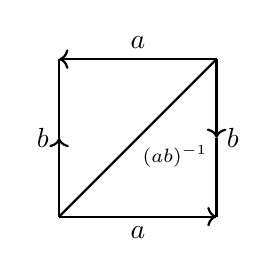
\begin{tikzpicture}[thick]
  \draw[->](0,0)--(0,1) node[anchor=east] {$b$};
  \draw[-](0,1)--(0,2);
  \draw[<-](0,2)--(1,2) node[anchor=south] {$a$};
  \draw[-](1,2)--(2,2);
  \draw[->](2,2)--(2,1)node[anchor=west] {$b$};
  \draw[-](2,1)--(2,0);
  \draw[<-](2,0)--(1,0) node[anchor=north] {$a$};
  \draw[-](1,0)--(0,0);
  \draw[-](0,0)--(2,2) node[yshift=-35, xshift=-15] {$\scriptstyle{(ab)^{-1}}$};
\end{tikzpicture}
\end{equation}
Here we have two $0$-chains $[a],[b]$ which are closed but $[(ab)^{-1}]=-[a]-[b]+\partial[\ldots]$. Therefore $H_{1}(T^{2})=\bbZ\oplus\bbZ$.

If we label the edges with the right group elements from $\bbA$ (so we put defects on the edges) and take a chain, we see that the closeness condition implies the group law
\begin{equation}
	\gamma=a[10]+b[20]+c[03]+\cdots
\end{equation}
then
\begin{equation}
	\left.\partial\gamma\right|_{[0]}=(a+b-c)[0]=0\implies a+b=c
\end{equation}
So a closed chain is in one-to-one correspondence with defects carrying group law. A chain $\gamma\in C_{d-p-1}(X,\bbA)$ is closed, then $\gamma$ corresponds to a $p$-form symmetry.

We also need to mod out for boundaries. Boundaries are nuclated whenever we have a loop in the network since they have to be closed by definition. Therefore, when we want to talk about defects, we not only require them to be closed but also mod out by nucleation which requires them to be in some homology group.

\subsection{Cohomology}
So we introduced the homology groups $\HH_j(X,\bbA)$ whose elements are closed chains which are not exact. We also found the physical correspondence of such objects: a $\gamma\in \HH_j$ is a newtork of $\bbA$-defects on a simplicial triangulation $\Delta(X)$ of some space-time manifold $X$\dots

We can now introduce the concept of \textit{co-chains}
\begin{defn}{Cochain}{}
	A co-chain $\nu$ is an element of 
	\begin{equation}
		C^j(X,\bbA)\equiv \mathrm{Hom}(C_j(X),\bbA)
	\end{equation}
	i.e. a map from chains to elements of an abelian group $\bbA$.
\end{defn}
As per the chains, cochains form an abelian group and we can define a differential
\begin{equation}
	\dd{}:C^j(X,\bbA)\rightarrow C^{j+1}(X,\bbA)
\end{equation}
which will act as expected: take $\nu\in C^j(X,\bbA)$, then
\begin{equation}
	\dd{\nu}(\gamma):=\nu(\partial\gamma)
\end{equation}
Clearly this is idempotent $\dd^2=0$. In components, by choosing a basis for $C_j(X)$, $\gamma=[i_0,\ldots, i_j]$ we have
\begin{equation}
	\nu\qty([i_0,\ldots, i_j])=\nu_{i_0\ldots i_j}\implies \dd{\nu}_{i_0\ldots i_j}=\sum_k (-1)^k \nu_{i_0\ldots i_{k-1}\;i_{k+1}\ldots i_j}
\end{equation}
Consider for example a $1$-cochain $\nu_{ij}$, we see that (using multiplicative notation)
\begin{equation}
	\dd{\nu}_{ijk}=\nu_{jk}\nu^{-1}_{ik}\nu_{ij}.
\end{equation}
Homology for cochains is called \textit{cohomology} and is given by the following co-chain complex
\begin{equation}
	\cdots\rightarrow C^j(X,\bbA)\xrightarrow{\dd}C^{j+1}(X,\bbA)\xrightarrow{\dd}C^{j+2}(X,\bbA)\xrightarrow{\dd}\cdots
\end{equation}
and
\begin{equation}
	\HH^j(X,\bbA)=\frac{\mathrm{Ker}(\dd_j)}{\mathrm{Im}(\dd_{j-1})}
\end{equation}
whose elements are flat connections which are not pure gauge.

On cohomology, we can define some natural operations
\begin{defn}{Cup-Product}{}
	Given a, possibly non-degenerate, pairing between abelian groups
	\begin{equation}
		(\;,\;):\bbA\times \bbB \rightarrow \bbD
	\end{equation}
	the \textit{cup product} is a product defined on co-cochains
	\begin{equation}
		\cup:C^j(X,\bbA)\times C^k(X,\bbB)\rightarrow C^{j+k}(X,\bbD)
	\end{equation}
	such that
	\begin{equation}
		(\mu \cup \nu)_{i_0,\ldots,i_{j+k}}\equiv (\mu_{i_0,\ldots, i_j},\nu_{i_j,\ldots, i_{j+k}})
	\end{equation}
\end{defn}
To have lift this to a good product in cohomology, we need it to be graded commutative. In general, given $A\in C^j, B\in C^k$
\begin{equation}
	\dd(A\cup B)=\dd{A}\cup \dd{B}+(-1)^j A\cup\dd{B}
\end{equation}
The product as defined on cochains is not, generally, graded commutative but the following
\begin{equation}
	A\cup B=(-1)^{jk}B\cup A+\dd{(A\cup_1 B)}+\dd{A}\cup_1 B+(-1)^j A\cup_1\dd{B}
\end{equation}
is graded commutative. The $\cup_1$ symbol is the Steenrod cup product and is another well defined product on cochains
\begin{equation}
	\cup_1:C^j\times C^k\rightarrow C^{j+k-1}
\end{equation}
This product is, on cohomology, graded commutative since $\dd{A}=0$, so we have defined a sensible product in cohomology.

Examples of reasonable parings are the following
\begin{itemize}
	\item Consider any abelian group $\bbA$ and $\bbB=\bbA^\vee\equiv \Hom(\bbA,\U(1))$ it's Pontrijagin dual. Elements of the Pontrijagin dual are just the characters of $\bbA$. Then the pairing is just given by
	\begin{equation}
		(a,\chi)=\chi(a)
	\end{equation}
	\item If both groups are $\bbZ_n$ then
	\begin{equation}
		(x,y)=xy\mod n
	\end{equation}
\end{itemize}
\subsection{Poincarè duality}
Poincarè duality over some space is an equivalence, if it exists, relating cohomology and homology on that space.\\
To do so, we need to introduce a method of adjoining chains and cochains. This is given by the cap product
\begin{defn}{Cap-product}{}
	Let $X$ be a topological space nd $\bbA$ some abelian group. The \textit{cap-product} is a bilinear map on homology and cohomology
	\begin{equation}
		\cap:H_j(X,\bbA)\times H^k(X,\bbA)\rightarrow H_{j-k}(X,\bbA),\qquad j>k
	\end{equation}
	defined by contracting a chain $\sigma\in C_j(X,\bbA)$ with a cochain $\mu\in C^k(X,\bbA)$ in the following manner
	\begin{equation}
		\sigma \cap \mu=\mu(\left.\sigma\right|_{[i_0,\ldots,i_k]})\left.\sigma\right|_{[i_k,\ldots,i_j]}
	\end{equation}
	Here the notation $\left.\sigma\right|_{[i_0,\ldots,i_k]}$ indicates the restriction of the simplicial map $\sigma$ to its face spanned by the vectors of the base.
\end{defn}
With this product at hand we can state the following theorem
\begin{thm}{Poincaré duality}{}
	If $X$ is a closed oriented $n$-mainifold with fundamental class $[X]\in H_n(X,\bbA)$, then the map 
	\begin{equation}
		\phi: H^k(X,\bbA)\rightarrow H_{n-k}(X,\bbA)
	\end{equation}
	defined by
	\begin{equation}
		\phi(\alpha)=[X]\cap \alpha
	\end{equation}
	is an isomorphism for all $k$.
\end{thm}
The relevance of this theorem in physics is that given a network of defects we have an associated gauge field and viceversa. So from $\gamma\in H_{d-p-1}(X,\bbA)$ we fin an $A\in H^{p+1}(X,\bbA)$. 

The idea of the proof is as follows: consider a triangulation $\Delta(X)$ and its dual $\overset{\vee}{\Delta}(X)$ constructed like a dual Bravais lattice in condensed matter
\begin{equation}
	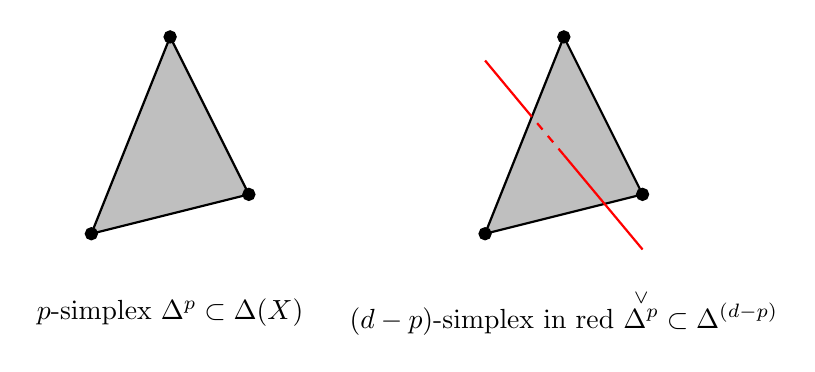
\begin{tikzpicture}[thick]
		\path [fill=lightgray,draw] (0,-.5) to (2,0) to (1,2) to (0, -.5);
		\filldraw[black] (0,-.5) circle (2pt) node[]{};
		\filldraw[black] (2,0) circle (2pt) node[]{};
		\filldraw[black] (1,2) circle (2pt) node[]{};

		\path [fill=lightgray,draw] (5,-.5) to (7,0) to (6,2) to (5, -.5);
		\draw[-, red] (7,-.7)--(6,0.5);
		\draw[dashed, red] (6,0.5)--(5.59,0.99);
		\draw[-, red] (5.59,0.99)--(5,1.7);
	  	\filldraw[black] (5,-.5) circle (2pt) node[]{};
	  	\filldraw[black] (7,0) circle (2pt) node[]{};
	 	\filldraw[black] (6,2) circle (2pt) node[]{};
		

		\node at (1,-1.5) {$p$-simplex $\Delta^p\subset \Delta(X)$};
		\node at (6,-1.5) {$(d-p)$-simplex in red $\overset{\vee}{\Delta^p}\subset \Delta^{(d-p)}$};
  \end{tikzpicture}
\end{equation}
In general the dual triangulation is not a triangulation. 

So for example, in $2d$ a $1$-simplex and it's dual are the following\\
\begin{minipage}[c]{0.3\linewidth}
	\centering
		\begin{tikzpicture}[auto,baseline=(A)]
			%%%%%%%%%%%%%% nodes %%%%%%%%%%
			\node (A) at (0,0) {$0$};
			\node (B) at (3,0) {$1$};
			\node (C) at (1.5,3) {$2$};

			\filldraw[black] (0,0) circle (2pt) node[]{};
			
		\end{tikzpicture}
	\end{minipage}\hfill
	\begin{minipage}[c]{0.5\linewidth}
	\begin{equation}
		[01]\xlongrightarrow{P}[\overset{\vee}{0},\overset{\vee}{1}]=P([01])
	\end{equation}
\end{minipage}
\chapter{Chern-Simons theory}
This chapter is basically a relaboration and expansion of \cite[Chapter 2]{Moor} which has also been covered in a four lectures series at TASI by Greg Moore on CS-theory. 

\section{\texorpdfstring{$U(1)$-Chern Simons Theory}{CS}}
A Chern-Simons theory is a Gauge theory with the following inputs
\begin{enumerate}
    \item A \textbf{Compact Lie group $G$}\footnote{Generalizations to Finite groups will be discussed In chapter \ref{ZNCS}}
    \item An \textbf{orientable $3$-Manifold} $\mathcal{M}_3$
    \item A \textbf{$G$-Principal Bundle $P \to \mathcal{M}$} with local connection $A_i \in \Omega(U_i) \otimes \mathfrak{g}$ ($\cup_{i} U_i = \mathcal{M}_3$)
\end{enumerate}
If the bundle $P \to \mathcal{M}_3$ can be trivialized\footnote{$P \simeq G \times \mathcal{M}_3$}, $\{A_i\}$ can be consistently patched together in a well defined global $\mathfrak{g}$-valued $1$-form $A$. The Chern-Simons action is:
\begin{equation}
    S_{\text{Chern-Simons}} = \frac{k}{8 \pi^2} \int_{\mathcal{M}_3} \text{Tr}(A \wedge d A + \frac{2}{3} A \wedge A \wedge A)
\end{equation}

\section{Quantization}
\subsection{Quantization Procedures}

\subsection{Mathematical Aside: Moment Map and Symplectic reduction}
Let $(\mathcal{M}, \omega)$ be a \textbf{symplectic manifold}. We are interested in studying the action $\phi_{(\cdot)}$ of some Lie group $G$ on $\mathcal{M}$ which preserves the symplectic form $\omega$:
\begin{equation}
	\label{sy}
    \phi_g^*(\omega) = \omega
\end{equation}
for any $g \in G$. Flows of this type are called \textbf{symplectomorphisms}. A simple example of those actions is provided by \textbf{Hamiltonian Vector Field} $X_f \in \Gamma(T \mathcal{M})$ associated to any $f \in C^{\infty}(\mathcal{M})$. Those vector fields are defined by the condition:
\begin{equation}
    \omega(X_f,\cdot) = \dd f
\end{equation}
which can be read in coordinates $(x^1,\cdots,x^{2n})$, as
\begin{equation}
    \omega_{ij} (X_f)^i = \partial_j f \to X_f^i = \omega^{ij} \partial_j f 
\end{equation}
where $\omega^{ij} \in \Gamma(T \mathcal{M} \otimes T \mathcal{M} )$ such that $\sum_j \omega^{ij} \omega_{jk} = \delta^{i}_k$. If we consider the group of diffeomorphisms generated by $X_f$, $\Phi_{X_f}^t$ ($t \in \mathbb{R}$), the condition \eqref{sy} is indeed satisfied because at any point $p \in \mathcal{M}$
\begin{equation}
   \mathcal{L}_{X_f} (\omega) = d \omega(X_f, \cdot) +  \cancel{(d \omega)}(X_f, \cdot , \cdot) = d^2 f =0
\end{equation}

In general, if $\xi \in \Gamma(T \mathcal{M})$ is the generator of the one group-parameter of symplectomorphism $\phi_{\exp(t T)}$ along some direction given by $T \in \mathfrak{g}$, using the same reasoning as above, it holds that:
\begin{equation}
    d \omega(\xi, \cdot) =0
\end{equation}
If $H^1_{\text{dR}}(\mathcal{M})= \{0\}$, then we can find a function $\mu(T) \in C^{\infty}(\mathcal{M})$ such that
\begin{equation*}
    \dd \mu(T) = - \omega(\xi, \cdot)
\end{equation*}
$\mu(T)$ is called the \textbf{charge} associated to the symmetry generated by the vector field $\xi$, because it generates $\phi_{\exp(t T)}$. Indeed
\begin{equation}
    \{ \mu(T), f\} = \omega^{ij} \partial_i \mu(T)\partial_j f = - \omega^{ij} \omega_{ik} \xi^i \partial_j f = \delta^j_k \xi^i \partial_j f = \xi^j \partial_j f = \xi(f) = \mathcal{L}_{\xi}(f)
\end{equation}
In more formal terms
\begin{defn}{Momentum Map}{}
   A Momentum Map is a linear assignment
  \begin{equation}
  \begin{aligned}
  	 \mu:  \mathfrak{g} &\to C^{\infty}(\mathcal{M})\\
	T &\mapsto \mu(T)
    \end{aligned}
\end{equation}
such that
\begin{equation}
     \phi_g^* \mu = \text{Ad}^*_g \mu
\end{equation}
where $\text{Ad}^*_g$ is the \textbf{coadjoint action} of $G$ on $\mathfrak{g}^*$ defined by
\begin{equation}
    \left \langle \text{Ad}^*_g \mu , T \right \rangle = \left \langle \mu , \text{Ad}_g T \right \rangle
\end{equation}
Equivalently, $\mu \in  C^{\infty}(\mathcal{M}) \otimes \mathfrak{g}^*$ by usual identification
\begin{equation}
    \left \langle \mu, T \right \rangle = \mu(T)
\end{equation}
\end{defn} 
Let's see some examples of momentum map.

\section{\texorpdfstring{$\mathbb{Z}_n$-Chern Simons theory}{ZnCS}}\label{ZNCS}

\chapter{The power of symmetry}
We will state a lot of QM examples with very formal language, which will help understand the fancy language also for the fancier examples. Start with very limited definition of symmetry: a global symmetry means having a unitary operator $U$ that commutes with the hamiltonian $UH=HU$ (also anti-unitary for time reversal but ok). The second condition is that the operators are in a faithful linear (acts like an ordinary rep, not up to phases like states) representation (there is no symmetry op. that acts trivially on everything) of the symmetry group. 

Every op. $O_{i}$ is mapped as 
\begin{equation}
	O_{i}\rightarrow U O_{i}U^{-1}=\sum_{j}R_{ij}(U)O_{j}
\end{equation}
where $R$ is the representation matrix of the symmetry group.

The modern way to talk about symmetry is to pretend that we couple the system to background gauge fields for the symmetry (it is not gauge, is global, acts on Hilbert space and operators). We consider the system as one point in a family of theories labelled by a background gauge field. The object of interest is 
\begin{equation}
	Z(A)=\int e^{-S(A)}
\end{equation}
where $A$ is a vector potential to the symmetry, for example $\U(1)$, and does not have to satisfy any classical eom. Then we ask what happens under a gauge transformation $A\rightarrow A^{g}$, is the partition function gauge invariant? It could happen that
\begin{equation}
	Z(A^{g})=Z(A)e^{-i\omega(A,g)}
\end{equation}
maybe we should add some terms to the action to get rid to that phase. If it is not possible, than we say that there is an anomaly. This has nothing to do with field theory, fermions and whatever, this is the minimal way of thinking about it.

The simplest example is the following: a single qbit or equivalently a $2$-level system or a complex fermion in QM
\begin{equation}
	i\int\psi^{\dagger}\partial_{t}\psi
\end{equation}
What is the global symmetry? Maybe a $\U(1)$ that rotates the fermions, but also charge conjugation $\bbZ_{2}$ and together they give $\OO(2)$. Option number two, we have a 2 dimensional Hilbert space so we can perform any $2\times 2$ commutes with the hamiltonian which is $H=0$ and so one might think that the symmetry is $\U(2)$. But we need to consider that the representation should be linear so we have to mod out by a $\U(1)$ phase of the projective representation on states $\U(2)/\U(1)=\SO(3)$. Notice that the symmetry is bigger than before. This is happens usually since the lagrangian does not exhibit the full symmetry of the system (this phenomenon is known as quantum symmetry).

Symmetries act projectively on the Hilbert space: we have a symmetry operator
\begin{equation}
	S(\vec{r})=e^{i\vec{r}\cdot\vec{s}},\qquad \vec{s}=\frac{1}{2}\vec{\sigma}
\end{equation}
this is how the $\SU(2)$ is realized on the Hilbert space. Since the action is by conjugation, we ask what are the conjugacy classes of $\SO(3)$. We limit ourselves
\begin{equation}
	g(\xi)=e^{i\xi s^{z}},\qquad g(\xi)\sim g(-\xi),\qquad g(\xi+2\pi)=-g(\xi)
\end{equation}
The action on the Hilbert space is with the minus which means that the symmetry is realized by the double cover $\SU(2)$. Notice that the adjoint action on the operators does not see the minus sign.

Now we take a gauge field $A$ for the $\SO(3)$ symmetry (it only has a time component in QM) and pick a gauge such that $A$ does not depend on $t$ (we take euclidean time)
\begin{equation}
	Z(\xi)= \Tr e^{-\beta H} g(\xi)=2\cos\qty(\frac{\xi}{2})
\end{equation}
since we have two states with opposite spin and the Hamiltonian is zero. This works for $Z(-\xi)=Z(\xi)$ but $Z(\xi+2\pi)=-Z(\xi)$. But what if we use
\begin{equation}
	g(\xi)=e^{i\xi s^{z}}\rightarrow e^{i\xi(s^{z}+\frac{1}{2})}
\end{equation}
by doing this there is not the minus sign anymore. But now I messed up the initial formula for $Z(\xi)$. Such a redefinition is called adding a counterterm and the freedom of moving the anomaly around is the freedom of adding counterterms. So here we cannot satisfy the full symmetry $\SO(3)$.

Consider now another example: the rotor. We start with the lagrangian
\begin{equation}
	L=\frac{1}{2}\dot{q}^{2}+\frac{\theta}{2\pi}\dot{q},\qquad q\simeq+2\pi
\end{equation}
the global symmetries are
\begin{equation}
\begin{split}
	&\U(1):q\rightarrow q+\alpha,\qquad\text{Is not }\bbR\text{ since }q\text{ is circle valued}\\
	&\bbZ_{2}:q\rightarrow -q,\quad \theta=0 \mod \pi
\end{split}
\end{equation}
These two combine into
\begin{equation}
	\OO(2)=U(1)\rtimes\bbZ_{2}
\end{equation}
so that $\bbZ_{2}$ acts on $\U(1)$. Let us do some QM
\begin{equation}
	p=\dot{q}+\frac{\theta}{2\pi}
\end{equation}
and
\begin{equation}
	H=p\dot q-L=\frac{1}{2}\qty(p-\frac{\theta}{2\pi})^{2}
\end{equation}
and the eigenvalues of $p\in \bbZ$ since $q$ is circle valued. The spectrum of the hamiltonian is
\begin{equation}
	E_{n}=\frac{1}{2}\qty(n-\frac{\theta}{2\pi})^{2}
\end{equation}
where we have degenerate states at $\theta=\pi,3\pi,\ldots$. Let us go over the simmetries
\begin{equation}
\begin{split}
	&q\rightarrow q+\alpha, \qquad\text{charge }Q=P\\
	&q\rightarrow RqR^{-1}=-q\\
	&RQR^{-1}=R(\dot{q}+\frac{\theta}{2\pi})R^{-1}=-Q+2\frac{\theta}{2\pi}
\end{split}
\end{equation}
For $\theta=2\pi$ we can redefine the charge $Q\rightarrow Q-\frac{\theta}{2\pi}$ but for $\theta=2\pi$ I cannot do it. For $\theta=0\mod 2\pi$ the symmetry is $\OO(2)$ and is realized linearly but for $\theta=\pi\mod 2\pi$ the symmetry is anomalous, is still $\OO(2)$ but is realized projectively. 

In terms of gauge fields
\begin{equation}
	L=\frac{1}{2}\qty(\dot{q}+A)^{2}+\frac{\theta}{2\pi}\qty(\dot{q}+A)+k A
\end{equation}
where the last part is a Chern-Simmons term in QM. Choose a gauge where $A$ is constant and compute the partition function: for $\theta=\pi$ in euclidean the only gauge invariant information is the following 
\begin{equation}
	e^{i\oint A_{euc}}=e^{i\xi}
\end{equation}
and compute
\begin{equation}
	Z(\xi)=\Tr e^{-\beta H}e^{i\xi (n+k)}=\sum_{n=-\infty}^{\infty}e^{-\frac{\beta}{2}\qty(n+\frac{1}{2})^{2}}e^{i\xi(n+k)}
\end{equation}
Moreover
\begin{equation}
	Z(\xi+2\pi)=Z(\xi),\qquad Z(-\xi)=Z(\xi)e^{-i(2k+i)\xi}
\end{equation}
so it acquires a phase which depends on the background gauge field $\xi$. So the $\bbZ_{2}$ is anomalous and is not realised properly. What are we going to do about it? We have many options
\begin{enumerate}
	\item That's it, it is what it is, $k\in\bbZ$
	\item Set $k=-1/2$. Now the $\bbZ_{2}$ is good but the $\U(1)$ is note
	\item Set $k=0$ and add a bulk $\exp\left(i\frac{\theta}{2\pi}\int F\right)$, so we add a $1$-dimensional space other than time and in the bulk there are only classical gauge fields which only keep track of the symmetries. In condensed matter this is called SPT (the system in the bulk is almost trivial, there are no dof but there is still a dependence on $F$). Even at $\theta=\pi$ by changing how we define $A$ in the bulk, we could get a minus sign which is what we are interested in.
\end{enumerate}
Now we want to go to the low energy theory. In our Hilbert space we have an infinite number of states and we are interested in the low lying states. At $\theta=\pi$ we have two degenerate states, we consider the $\beta\rightarrow\infty$ limit on the partition function and consider the saddle point
\begin{equation}
	Z(\xi)\rightarrow e^{-\frac{\beta}{8}}e^{i\xi k}(1+e^{i\xi})
\end{equation}
and now we can consider different values of $k$ and see what happens. For the two interesting values of $k$ the behavior is the same as the qubit system. There is one crucial difference: the rotor system has $\OO(2)$ symmetry, but the two level system as $\SO(3)$ symmetry. This is a general statement, the symmetries of a system in the IR and UV do not have to be the same.
\begin{equation}
	G_{UV}\xrightarrow{\phi} G_{IR}
\end{equation}
the map might not be so trivial $\ker \phi \neq\{0\}$ since some symmetries in the UV might act trivially in the IR. In the case of the rotor we have an emergent symmetry (in condensed matter) or accidental symmetry (in HEP)

We would like $Z$ to be a function on the parameter space: a circle $\xi$ modded out by $\bbZ_{2}$, so is like a line segment. We would like the partition function to be an actual function of $\xi$ but we cannot do that. Even if the parameter space is a segment, the partition function is not actually a function of the segment, it is a chapter of a line bundle over this space. The minus sign reflects that.

There is another thing: the system has an anomalous $\OO(2)$ symmetry. The anomaly guarantees that all the states are in a projective rep and the projectiveness has to be the same because the operators are in linear representations. Every state is two-fold degenerate. The IR observer says that every state has to be two-fold degenerate so also the ground state has to be. In some cases this is not trivial to see from UV to IR. The right way is to see that anomalies have to match between UV and IR.

Consider again the rotor system but add a $\bbZ_{2}$-invariant potential $V(q)$ which is also invariant under a shift of $\pi$ in $q$. For example, one that works is
\begin{equation}
	V(q)=\cos 2q+5.4\cos 4q
\end{equation}
In general now I cannot solve the system. What happens to the symmetries? For $\theta=0 \mod \pi$, the symmetry is $\bbZ_{2}\times\bbZ_{2}$ with $q\rightarrow -q$ and $q\rightarrow q+\pi$ where, again $q$ is circle valued. For $\theta=\pi$ there is an anomaly between the two $\bbZ_{2}$. So the symmetry is realized projectively. Every state is two-fold degenerate. In the IR we don't know how to diagonalize the Hamiltonian but still we know that the ground state will be degenerate. So the system has to be realized projectively even in the IR.

A realization of the $\bbZ_{2}^{2}$ is given by $\sigma^{x},\sigma^{y}$ since consider the generators of the two $\bbZ_{2}$ beign $A,B$. These have to satisfy the relations
\begin{equation}
	A^{2}=B^{2}=1,\qquad AB=-BA
\end{equation}
where the second one comes from projectiveness. We see that the two Pauli matrices satisfy this relations since they anticommute and square to one. All the representations are two dimensiona. There is no one-dimensional representation since if we take $A=B=\pm1$ the second equation is not solved.

\section{Higher symmetries}
When the operators are supported on higher dimensional manifolds, the group action is preserved but the unitary operators associated with the symmetries live on a higher codimension manifold. When the symmetry is continuous, there is a direct definition of the unitary in terms of the conserved currents.\\
These symmetries act exactly as normal symmetries and are useful for much of the same reasons.

We give many examples: the first one is a free field theory, a $\U(1)$ gauge theory in $3+1$ dimensions. The two $1$-form symmetries are $\U(1)^{2}$ which give a current that generates the unitary. The two currents are 
\begin{equation}
	\frac{2}{g^{2}} \star F,\qquad \frac{1}{2\pi} F
\end{equation}
Integrating it over a surface we get the electric and magnetic fluxes. How do they act on different fields? Just compute the commutation relations. The electric symmetry just shifts the vector potential
\begin{equation}
	A\rightarrow A+\xi,\qquad \dd{\xi}=0
\end{equation}
The magnetic symmetry does not act in a simple way on $A$, but acts simply on the dual photon by shift again. The operators are
\begin{equation}
	U_{g_{\alpha}=e^{i\alpha},g_{\eta}=e^{i\eta}}(M)=e^{i\frac{\alpha}{2\pi}\int_{M}F+i\frac{2\eta}{g^{2}}\int_{M}\star F}
\end{equation}
it is called Gukov-Witten operator. The charged objects are Wilson and 't Hooft lines $W_{n}(L),H_{m}(L)$ where $n,m$ are electric and magnetic charges of the lines.

The next example is in $2+1$ dimensions and is a $\U(1)$ Chern-Simons theory
\begin{equation}
	\cL=\frac{N}{4\pi}\int A\dd{A}
\end{equation}
This theory has a $1$-form symmetry with the shift by a constant. By doing this, we need the lagrangian to be gauge invariant
\begin{equation}
	A\rightarrow A+\frac{1}{N}\epsilon,\qquad \dd{\epsilon}=0
\end{equation}
and moreover $\epsilon$ has integer periods. The $1$-form is therefore $\bbZ_{N}$. Here the lines also carry an electric charge, but is a slightly different charge. By looking at the EOM of the field with a source, we say that the magnetic field is a delta function on the source and consequently by going around the line we get an holonomy depending on the charge. The charge operator is also the charged operator. This is a statement that the $\bbZ_{N}$ symmetry is anomalous. Various subgroups could be anomaly free.

Next example is a $3+1$ dimensional $\U(1)$ gauge theory with a scalar field with charge $N$. The magnetic symmetry remains the same since $F$ is still a conserved charge. But the electric symmetry now is broken since when we shift $A$ in the covariant derivative, the kinetic term for the scalar field is not invariant unless we shift by something which is $N$-times the basic unit. So the electric symmetry is a $\bbZ_{N}$. The charged objects are the Wilson lines, but the theory has also dynamical scalar fields with charge $N$. The line operators can now attach to the scalar fields.

Next example is $3+1$ dimensional $\SU(N)$ gauge theory without matter. Now the electric symmetry is $\bbZ_{N}$ and no magnetic symmetry. We can shift the gauge fields by a flat $\bbZ_{N}$ connection. Take any lattice configuration and we put at every link an $\SU(N)$ matrix, then we multiply each link by $e^{2\pi i/N}\mathbf{1}$. We do it in such a way that the plaquettes do not change. This is a symmetry.\\
Every line carries a rep of $\SU(N)$ but we can attach a gluon to it and change it's charge, so we are just interested in the N-ality of the line.\\
There are no t' Hooft operators, they have to be attached to surfaces, so there is no magnetic symmetry.

Next example is $3+1$ dimensional $\SU(N)$ with quarks in the fundamental rep $\mathbf{N}$. There is still no magnetic symmetry and the electric symmetry is screened, therefore there is no electric symmetry also. At large N, the quarks do not participate in the dynamics so the $1$-form symmetries comes back.

Next example is a $3+1$ dimensional $\text{PSU}(N)=\SU(N)/\bbZ_{N}$ (we have more possible bundles where the transition functions are closed) and can be thought of as gauging the $1$-form in the other example. In this theory we cannot add the quarks since the $\text{PSU}(N)$ does not have a rep which is charged under $\bbZ_{N}$. We also get a quantum symmetry\footnote{From the orbifold point of view this is the symmetry that acts on the twisted sectors} which is a $\bbZ_{N}$  $1$-form magnetic symmetry. The 't Hooft lines come back.

Last example is the $\bbC P^{n}$ model (sigma model with target space this manifold). This has instantons since this manifold has non-trivial $2$-cycles. in $2+1$ dimensions it has skyrmions. In $3+1$ dimensions there are strings and therefore there is a $1$-form symmetry. $\bbC P^{n}$ has a Kahler form which can be integrated to find the charge. Here there is no gauge field.
\chapter{Rep theory of categorical symmetries}
How do categorical stymmetries act on and organiser thespectrum of operators in QFT? We are interested in genuine operators in the QFT, non-topological. The known idea is from representation theory as it usually applyies on invertible symmetries. Local op transform in some rep of a local symmetry, but also the same for lines which transform under rep of a one-form symmetry. This can be pushed to higher representations when zero form symmetries act on line defects, $2$-representations. 

This gives us an organising principle. But how do we do that for non-invertible symmetries? We have some (higher) fusion category which encompasses the action on some operators. Studying twisted sectors is key: consider local op attached to topological lines. We might have local operators attached to top lines, or line attached to topological surface etc. 

The answer, as alwyas, is conclusive for fusion categories $\cC$ in $d=2$: two answers
\begin{itemize}
	\item internal: representations of a tube algebra $\cA$. This is just the representation theory of an algebraic structure associated to the category.
	\item sandwitch construction: topolofical lines in $TV_\cC$. Via this construction all the twisted sector operators are attacched to a given topological line in the $3d$ theory.
\end{itemize}
Representations of the tube algebra are 
\begin{equation}
	\mathrm{Rep}(\cA)\equiv Z(\cC)
\end{equation}
where the right is the Drinfeld center of the category. 

Can this be extended to higher dimensions? Or also consider twisted secotr of nigher extended operators? Representtionf of $S^{d-n}$ Tube $n$-algebra, or $n$-dimensional operators in $TV_\cC$.
\begin{equation}
	\mathrm{nRep}\cA_{S^{d-n}}(\cA)\equiv \int_{S^{d-n}}\cC
\end{equation}

\section{Recap of $2d$}
The setup is as follows 
\begin{itemize}
	\item Spherical fusion category $\cC$: objects that correspond to topological lines $x,y,\ldots$. There is a notion of the dual with orientation reversal and object have fusion rules 
	\item $\pi_0(\cC)=$ Simple objects / isomorphisms. Fusion ring of category
	\item $x$-twistet local operator $x\in \pi_0(\cC)$
	\item $S^1$ tube action: lasso diagrams
\end{itemize}

The tube algebra is 
\begin{itemize}
	\item Finite semi-simple algevra $\cA_{S^1}(\cC)$
	\item Generated by morphisms in $\cC$ 
	\begin{equation}
		\psi:\cA\otimes x\rightarrow y\otimes \cA
	\end{equation}
	\item Product from horizontal composition
	\item Twisted local operators transform in irreps of this algebra. There is more structure
	\begin{equation}
		\mathrm{Rep}\cA_{S^1}(\cC)\quad \text{is a braided fusion category}
	\end{equation}
\end{itemize}
This is not an internal algebra of the category. 
\chapter{Seiberg--Witten theory}
\section{Susy algebra}
The susy algebra in $4d$ is generated by a certain number of Weyl spinors 
\begin{equation}
	Q_{\alpha}^{i},\quad\Tilde{Q}_{\dot\alpha, j},\qquad \alpha,\dot\alpha=1,2;\quad i,j=1,\ldots,\cN
\end{equation}
whose algebra is 
\begin{equation}
	\acomm{Q_{\alpha}^{i}}{\tilde{Q}_{\dot\beta,j}}=\delta^{i}_{j}\sigma^{\mu}_{\alpha\dot\beta}P_{\mu}
\end{equation}
where $\sigma^{\mu}=(1,\vec{\sigma})$ are Pauli matrices and $P_{\mu}$ is the four momentum. The rest of usual anticommutators are
\begin{equation}
	\acomm{Q_{\alpha}^{i}}{Q_{\beta}^{j}}=\acomm{\tilde{Q}_{\dot\alpha,i}}{\tilde{Q}_{\dot\beta,j}}=0
\end{equation}
moreover there are all the other bosonic symmetries like Poincarè and internal symmetries. This algebra can be extended when we have conformally invariant theories (in that case, the anticommutator of two different supercharges contains also the special conformal transformation generator). There could also be some central extension to the anticommutators of the same kind of supercharges.

Now we discuss irreducible representations of this algebra. We look at states of positive mass $m>0$ by going to the rest frame where $P_{\mu}=(M,0,0,0)$ and there fore the algebra is
\begin{equation}
	\acomm{Q_{\alpha}}{\tilde{Q}_{\dot\beta}}=\delta^{i}_{j}\delta_{\alpha\dot\beta}M,\qquad \acomm{Q_{\alpha}}{Q_{\beta}}=\acomm{\tilde{Q}_{\dot\alpha}}{\tilde{Q}_{\dot\beta}}=0
\end{equation}
So we have the algebra for $2\cN$ fermion creation and annhilation operators. An irreducible rep has dimension $2^{2\cN}$.

Consider the case of $m=0$. The best we can do is $P_{\mu}=(E,0,0,E)$, considering a particle moving in the $z$ direciton. Then the algebra looks like the following (using the usually normalized $\sigma^{z}$)
\begin{equation}
	\acomm{Q_{\alpha}^{i}}{\tilde{Q}_{\dot\beta,j}}=\delta^{i}_{j}\delta_{\alpha\dot\beta}\,\mqty(1&0\\0&0)_{\alpha\dot\beta},\qquad \acomm{Q_{\alpha}}{Q_{\beta}}=\acomm{\tilde{Q}_{\dot\alpha}}{\tilde{Q}_{\dot\beta}}=0
\end{equation}
The main change is that the unit matrix whose eigenvalues are both one has been changed by a matrix whose one of the eigenvalues is zero. In lorentz signature, $\tilde{Q}=Q^{\dagger}$ is the hermitian adjoint of $Q$. If we set $\alpha=\dot\beta=2$ we get
\begin{equation}
	\acomm{Q_{2}^{i}}{\tilde{Q}_{2,i}}=0\implies \acomm{Q_{2}^{i}}{Q^{\dagger}_{2,i}}=0
\end{equation}
with no implicit sum on $i$. We have an operator whose anticommutator with it's adjoint is zero. But the anticommutator of an operator with is adjoint is positive definite. Therefore the only possibility is that on these states with $M=0$ $Q_{2}=\tilde{Q}_{2}=0$.\\
So instead of $2\cN$ creation and annihilation operators, we jet just $\cN$. So an irreducible rep has dimension $2^{\cN}$. With CPT, sometimes, $2\times 2^{\cN}$. If $\cN$ is not small, notice that $2^{2\cN}>2\times 2^{\cN}$. When this is true, some funny things are going to happen.

Let us look at small values of $\cN$. Start with the massless $\cN=1$. A massless particle is in an irrep of the Poincarè group labelled by it's helicity $j$.
The creation and annihilation operator are spinors $j_{z}=\pm 1/2$ therefore they raise and lower the helicity by half a unit. CPT reverses the sign of helicity so if we have a multiplet with helicity $j_{1},j_{2}$, we also have the states with $-j_{1},-j_{2}$.\\
For $\cN=0,1$ we always need four states. Since we are not interested in theories of gravity, but only gauge theory, we will consider reps with helicity $|j|\le1$ and there are only two possible massless reps
\begin{equation}
\begin{split}
	&(-j_{2},-j_{1},j_{0},j_{1},j_{2})\\
	\text{Vector Multiplet: }&(-1,-1/2,0,1/2,1)=(1,1,0,1,1)\\
	\text{Chiral Multiplet: }&(-1,-1/2,0,1/2,1)=(0,1,2,1,0).
\end{split}
\end{equation}
This spectrum of chiaral multiplet has $4$ states which is how many we need for a massive multiplet. And in fact this multiplet can get a mass in a completely susy fashion. The vector multiplet cannot since a massive vector has helicity zero which is not in the multiplet, it can get a mass with Higgsing.


Consider now $\cN=2$ in the massless case. The basic state, considering CPT, is as follows
\begin{table}[H]
\begin{tabular}{c|cccc}
	\text{N.States}&1&2&1&\\
	\hline
	\text{Helicity}&-j&$-j+\frac{1}{2}$&-j+1&$-j+\frac{3}{2}$
\end{tabular}
\end{table}
CPT means, first of all, that the quantum states are real. Whatever is the algebra of observables, their rep in the Hilbert space is real from CPT. Half of the $Qs$ are zero. The non-zero ones are four $2Q,2\tilde{Q}$ hermitian, by combination of these. These four generate a Clifford algebra. {\color{red}{Qui la registrazione è tagliata, comincia a parlare dei multipletti corti e lunghi in base alle estensioni centrali della superalgebra.}}

\section{\texorpdfstring{Most basic $\cN=2$ renormalizable gauge theory}{Most basic N=2}}
Beside free chiral theory, the most basic theory is a theory of only vector multiplets. The field content is: a vector $A$, two fermions $\lambda^{1,2}$, and a complex scalar $\phi$. We can construct three theories with this: the first is by hand starting with $\cN=1$ (a $\cN=2$ hypermultiplet is a vector+chiral multiplet in $\cN=1$).

Write down simplest $\cN=1$ action and claim that actually is $\cN=2$
\begin{equation}
	\int \dd[4]{x}\dd[2]{\theta} \Tr W_{\alpha}W^{\alpha}=\frac{1}{e^{2}}\int\dd[4]x\Tr\qty(F_{\mu\nu}^{2}+i\bar\lambda^{1}\slashed{D}\lambda^{1}+D^{2})
\end{equation}
plus we have a part for the adjoint chiral $\Phi$
\begin{equation}
\begin{split}
	\int\dd[4]{x}\dd[4]\theta\Tr\bar\Phi e^{V}\Phi=\frac{1}{e^{2}}\int\dd[4]{x}\Tr\Big(&D_{\mu}\bar\phi D^{\mu}\phi+\bar\lambda^{2}\slashed{D}\lambda^{2}+D\comm{\phi}{\bar{\phi}}\\
	&+\comm{\bar\lambda^{1}}{\bar\lambda^{2}}\phi+\comm{\lambda^{1}}{\lambda^{2}}\bar\phi\Big)
\end{split}
\end{equation}
Remember that $\lambda$ has one chirality and $\bar\lambda$ has the opposite chirality. Just Lorentz invariance does not tell us if we have to take the Yukawa coupling of $\lambda s$ with $\phi$ or $\bar\phi$. This is fixed by internal symmetries $\U(1)\times\U(1)_{R}$
\begin{equation}
	\U(1):\Phi\rightarrow e^{i\alpha}\Phi
\end{equation}
fixes the right product. The $R$-symmetry acts on the superspace as
\begin{equation}
	x\rightarrow x,\quad \theta\rightarrow e^{i\beta}\theta,\quad\bar\theta\rightarrow e^{-i\beta}\bar\theta
\end{equation}
There is a slightly less trivial $R$-symmetry, by combining it with the other $\U(1)$ such that
\begin{equation}
	\phi\rightarrow\phi,\qquad \lambda^{2}\rightarrow e^{-i\beta}\lambda^{2},\qquad \bar\lambda^{2}\rightarrow e^{i\beta}\bar\lambda^{2},\qquad \lambda^{1}\rightarrow e^{i\beta}\lambda^{1},\qquad \bar\lambda^{1}\rightarrow e^{-i\beta}\bar\lambda^{1}
\end{equation}
Consider the Yukawa term
\begin{equation}
	\Tr \epsilon_{ij}\epsilon^{\alpha\beta}\comm{\lambda_{\alpha}^{i}}{\lambda_{\beta}^{j}}\bar\phi
\end{equation}
It was already antisymmetric in the lorentz indices $\alpha$ but is also antisymmetric in the gauge indices because the coupling came from the gauge coupling of the adjoint representation. Therefore, since the coupling of the gluons involve commutators of the generators of the Lie algebra, by extending with susy we get more commutators. So the superpartner to the gauge field get the commutator.\\
So this object is also antisymmetric in the internal indices. So by no added cost, the lagrangian has a bigger global symmetry $\SU(2)$ which acts only on fermions
\begin{equation}
	\mqty(\lambda^{1}\\\lambda^{2})\rightarrow M\mqty(\lambda^{1}\\\lambda^{2})
\end{equation}
with $\det M=1$. But we can relax this condition by taking
\begin{equation}
	\phi\rightarrow \det M\, \phi
\end{equation}
where now $M\in \U(2)$. So we actually have a $\U(2)$ global symmetry. Of course $\U(1)\times \U(1)$ is the maximal torus of $\U(2)$, the diagonal part of the subgroup which was manifest since the start.\\
The realization by $\cN=1$ enabled us to see the diagonal part of $\U(2)$. This $\U(2)$ symmetry does not commute with the $\cN=1$ susy. Afterall
\begin{equation}
	\delta A_{\mu}=\bar\epsilon \gamma_{\mu}\lambda^{1}+\cdot
\end{equation}
but we have a $\U(2)$ that mixes $\lambda^{1}$ with $\lambda^{2}$. So we have an added symmetry which puts the two on the same ground and we get the $\cN=2$ generalization
\begin{equation}
	\delta A_{\mu}=\sum_{i=1,2}\bar\epsilon_{i}\gamma_{\mu}\lambda^{i}+\cdots
\end{equation}
Of course one has to add all the other transformations.
\subsection{Dynamics}
We want to find the potential energy for the theory which is done by integrating the auxilliary field $D$ over the EOMs. By doing so one gets
\begin{equation}
	V(\phi,\bar\phi)=e^{2}\Tr\qty( i\comm{\phi}{\bar\phi}^{2})
\end{equation}
the $i$ makes the commutator hermitian so that the trace is positive. So
\begin{equation}
	V=0\iff \comm{\phi}{\bar\phi}=0
\end{equation}
so that the $\phi$ matrix commutes with it's hermitian which is equivalent to saying that the hermitian and antihermitian part of $\phi$ commute with each other. They can be simultaneously diagonalized by a gauge transformation. Consider $G=\SU(2)$ gauge for example
\begin{equation}
	\langle\phi\rangle=\mqty(a&0\\0&-a),\qquad a\in\bbC
\end{equation}
but $a$ is not quite gauge invariant because we can make another gauge transformation which exchanges the two eigenvalues. What is gauge invariant is 
\begin{equation}
	\Tr \phi^{2}=2a^{2}\equiv u
\end{equation}
Now $u$ is a compelx parameter that labels the possible classical vacua of the theory. But after quantum corrections it is also true that $u$ labelles the quantum vacuas.

In the complex $u$ plane, we have a special point of unbroken gauge symmetry $u=0$. But on a generic point the gauge group is broken to $\U(1)$. We understand well the $\U(1)$ gauge theories, which just generate Coulomb forces. In the other cases, we have strong gauge dynamics which is very difficult to understand. Because of asymptotic freedom, for large $u$ the classical picture is valid, but for small $u$ we have to understand the strong dynamics of the theory.
\subsection{Spectrum}
Consider $u\neq 0$. The massless states are the same theory for $\U(1)$: massless vector multiplet which has $8 $ states
\begin{table}[H]
\begin{tabular}{c|ccccc}
	\multirow{ 2}{*}{N. States} & - & - & 1 & 2 & 1  \\
	& 1 & 2 & 1 & - & - \\
	\hline
	\text{Helicity}&-1&$-\frac{1}{2}$&0&$\frac{1}{2}$&1
\end{tabular}
\end{table}
and then we have a massive $W^{+}$ boson which corresponds to strictly upper triangular matrices. On the other hand, the reps didn't become bigger just because they are massive; there are still $8$ states. So there has to be a central charge! [Olive, Witten; Phys Lett...]\\
One can calculate the anticommutator
\begin{equation}
	\acomm{Q_{\alpha}^{i}}{Q_{\beta}^{j}}=\frac{1}{e^{2}}\int\dd[3]x \partial_{i}(\phi F_{0i}^{+})
\end{equation}
where 
\begin{equation}
	F_{0i}^{+}=\frac{1}{2}\qty(F_{0i}+\frac{\epsilon_{ijk}}{2}F_{jk})\implies \vec{F_{0i}^{+}}=\frac{1}{2}\qty(\vec{E}_{i}+i\vec{B}_{i})
\end{equation}
Of course being an integral of a total derivative, one can write it as a surface term at infinity, but what are those surface terms? The electric and magnetic fields at infinity
\begin{equation}
	F_{0i}^{+}=\frac{1}{2}\qty(F_{0i}+\frac{\epsilon_{ijk}}{2}F_{jk})=a\qty(Q_{el}+\frac{i}{e^{2}}Q_{mag})	
\end{equation}
it is clear from the normalization is that the $e^{2}$ factor cancels for the electric chage, while it does not for the magnetic charge. Classialy
\begin{equation}
	Z=a\qty(Q_{el}+\frac{i}{e^{2}}Q_{mag})	
\end{equation}
therefore
\begin{equation}
	M\ge \abs{Z}=\abs{a}\sqrt{Q_{el}^{2}+\qty(\frac{Q_{mag}}{e^{2}})^{2}}
\end{equation}
For BPS (short) representations 
\begin{equation}
	M= \abs{Z}=\abs{a}\sqrt{Q_{el}^{2}+\qty(\frac{Q_{mag}}{e^{2}})^{2}}
\end{equation}
so for $W$-bosons
\begin{equation}
	M= \abs{Z}=\abs{a}\abs{Q_{el}}
\end{equation}
and this is just the standard Higgs formula, the mass of the $W$-boson is proportional to the value of the Higgs vev $a$.

The factor of $i$ in the central charge for the magnetic charge is very important since in lorentz signature the curvature field is complex and is relevant since in the mass, without the factor of $i$, we would have had a mixed term between electric and magnetic charge which is odd under CP since the two charges transform in an opposite way. We could have violated CP by turning on a $\theta$-angle. This would not spoil susy, but it the cross term would be there since CP is explicitly broken.

\section{\texorpdfstring{The other way of constructing $\cN=2$ theory}{Other Way}}
We are going to consider minimal SYM in $d$ dimensions. The only fields are the gauge field $A_{\mu}$ and the fermion $\lambda$. We take the smallest fermion in $d$ dimensions which is allowed by Lorentz invariance. The lagrangian is
\begin{equation}
	\cL = \frac{1}{e^{2}}\int \dd[4]{x}\Tr\qty(F_{\mu\nu}^{2}+\bar\lambda i\slashed{D}\lambda)
\end{equation}
If the lagrangian is supersymmetric it has to be invariant under
\begin{equation}
	\delta A_{\mu}=\epsilon\Gamma_{\mu}\lambda,\qquad \delta\lambda=\Gamma^{\mu\nu}F_{\mu\nu}\epsilon
\end{equation}
where $\Gamma_{\mu}$ is the Dirac matrices in $d$-dimensions. By plugging this variation, one can show that the term linear in $\lambda$ cancels in any dimensions
\begin{equation}
	4\int\dd[4]{x}\Tr \qty(F_{\mu\nu}D^{\mu}(i\bar\epsilon\Gamma^{\nu}\lambda)+\frac{1}{2}\bar\lambda i\Gamma^{\mu}D_{\mu}(\Gamma^{\alpha\beta}F_{\alpha\beta}\epsilon))=0
\end{equation}
This can be shown by using the algebra of the $\Gamma$ matrices, practically since
\begin{equation}
	\Gamma^{\mu}\Gamma^{\alpha\beta}=\Gamma^{\mu\alpha\beta}+g^{\mu\alpha}\Gamma^{\beta}-g^{\mu\beta}\Gamma^{\alpha}
\end{equation}
it decomposes in symmetric and anti-symmetric parts. Using Bianchi identity and integration by parts we can show that the two contributions cancel.

There is actually a part which is cubic in $\lambda$ because we can take the part in the gauge field inside $\slashed{D}$ and vary that
\begin{equation}
	\frac{\delta}{\delta A}\bar\lambda\Gamma^{\mu}\comm{A_{\mu}}{\lambda}=f^{abc}\lambda^{\alpha}_{a}\Gamma_{\mu\alpha\beta}\lambda^{\beta}_{c}(\Gamma^{\mu})_{\rho\sigma}\lambda_{c}^{\rho}\epsilon^{\sigma}
\end{equation}
The only hope for this to be zero is that
\begin{equation}
	\Gamma_{\mu\alpha\beta}\Gamma^{\mu}_{\rho\sigma}+\text{symm }\alpha\beta\sigma=0
\end{equation}
which is true only if $d=3,4,6,10$.\\
The $4d$ case is just $\cN=1$ SYM in four dimensions, for today we consider the $6d$ case. Therefore we have a $6d$ supersymmetric lagrangian but we wanted an $\cN=2$ in four dimensions. We just brutally take the fields independent of the last two dimensions
\begin{equation}
	t\,x^{1}\,x^{2}\,x^{3}\quad x^{4}\,x^{5}
\end{equation}
we let
\begin{equation}
	\phi=A_{4}+iA_{5},\qquad A_{\mu=0,1,2,3},\qquad \lambda=2\text{ spinors in }d=4 
\end{equation}
Note, $\cN=4$ in $4d$ can be constructed in the same way starting from $10d$.

This second construction makes it clear why there should be a central extension to the susy algebra
\begin{equation}
	\acomm{Q_{\alpha}}{Q_{\beta}}=\sum_{\mu=0}^{5}\sigma_{\alpha\beta}^{\mu}P_{\mu}=\sum_{\mu=0}^{3}\sigma_{\alpha\beta}^{\mu}P_{\mu}+\sum_{\mu=4}^{5}\sigma_{\alpha\beta}^{\mu}P_{\mu}
\end{equation}
but what are the two more terms? The momentum commutes with the momentum and the supercharges, and they commute with the $4d$ Lorentz transformations which is all that we got in $4d$. So they become central charges! In fact they become the electric charge.

Let us be more specific on the nature of $\lambda$. In $6d$ we would have $6$ gamma matrices that we can combine into three creation and annihilation operators
\begin{equation}
\begin{array}{ccc}
	\Gamma_{0}+i\Gamma_{1}&\Gamma_{2}+i\Gamma_{3}&\Gamma_{4}+i\Gamma_{5}\\
	\Gamma_{0}-i\Gamma_{1}&\Gamma_{2}-i\Gamma_{3}&\Gamma_{4}-i\Gamma_{5}	
\end{array}
\end{equation}
If one just tries to represent the Clifford algebra, there would be $8$ states. But we wanted the smallest fermion. In $6d$ we can ask that the chirality operator, product of all gammas, on $\Gamma^{0}\cdots\Gamma^{5}\lambda=+\lambda$ since 
\begin{equation}
	(\Gamma^{0}\cdots\Gamma^{5})^{2}=1
\end{equation}
but in four dimensions this squares to $-1$ so it's eigenvalues are $\pm i$ and are exchanged by CPT. In $4d$ the hermitian adjoint of the spinor is the other spinor. But in $6d$ the square is $+1$ so $\lambda$ can obey a chirality condition so half number of states $=4$. And one might think that $\lambda$ has only four components. It is true that $\SO(1,4)$ has a $4d$ representation, call it Spinor$_{+}$ bus it's pseudo-real. Since it is pseudo-real one needs to double it taking an $8d$ rep.\\
So the smallest rep has $8$ real components. So the susy generator $\epsilon$ also has $8=2\times 4$ components and so $\cN=2$. In four dimensions the relations is 
\begin{equation}
	(\Gamma^{0}\Gamma^{1}\cdots\Gamma^{3})\lambda=-\Gamma^{4}\Gamma^{5}\lambda
\end{equation}
and the same for $\epsilon$.

Let us consider $\lambda^{\alpha}$ as $\lambda^{a\,x}$ where $a=1,\ldots,4$ is an $\SO(1,5)$ index and $x$ there since we double it to make it real, so now we have $\SU(2)$ index.\\
So we could write the $\lambda$ part of the lagrangian in more details
\begin{equation}
	\epsilon_{xy}\lambda^{ax}\Gamma_{ab}^{\mu}D_{\mu}\lambda^{by}
\end{equation}
which is manifestly $\SO(1,5)$ and $\SU(2)$ invariant. We discovered an $\SU(2)$ symmetry which only acts on fermions! And we also have a $\U(1)_{R}$ symmetry which acts on bosons and fermions: set the charge of $A_{4},A_{5}$ to have charge $\pm1$ so that the fermion $\lambda$ has charge $\pm 1/2$. The $\SU(2)_{R}$ acts only on $\lambda$. To show that the model is actually supersymmetric we need the identity
\begin{equation}
	\lambda^{\alpha}\lambda^{\beta}\lambda^{\gamma}\gamma^{\mu}_{\alpha\beta}\gamma_{\mu\gamma\delta}\epsilon^{\delta}+(\alpha\beta\gamma)=0
\end{equation}
which with the explicit indices is
\begin{equation}
	\lambda^{a_{1}x_{1}}\lambda^{a_{2}x_{2}}\lambda^{a_{3}x_{3}}\ldots\epsilon^{a_{4}x_{4}}+(\alpha\beta\gamma)=0
\end{equation}
We have $4$ guys which transform in the $4d$ rep of $\SO(1,5)$, and the only invariant that we can make is with the completely anti-symmetric symbol $\epsilon_{a_{1}a_{2}a_{3}a_{4}}$.\footnote{It can be proven by using the fact that the complexified $\SO(1,5)$ is just $\SL(4)$} We are trying to make a completely symmetric object but there is a completely anti-symmetric object. So we have to anti-simmetrize in the $\SU(2)$ indices . But there is no way of doing it, so the object is zero and the model is supersymmetric.

We need to find the other term in the central charge of the susy algebra. There is another kind of small rep we need to understand for the model. Discuss things we can see at weak coupling. What can we understand of the spectrum of the model at weak coupling? We have two types of particles at weak coupling: thew ones coming from the oscillations (each field gives a particle), and then we can quantize classical lumps (classical solitons). We take our non-linear field equations and find a solution $\Phi(\vec{x})$ which is independent of time (We want classical ground states which are independent of time so tu avoid kinetic energy and make them stable) and we quantize.\\
A classical solution is some kind of stable lump. For simplicity we assume that the classical solution is unique except from what we can deduce by symmetry. We have a family of solution
\begin{equation}
	\Phi(\vec{x})=\Phi(\vec{x}+a)
\end{equation}
quantizing it means that we need to find a quantum wavefunction that depends on $a$. An interesting one is
\begin{equation}
	\Psi(a)=\exp\qty(i\vec{p}\cdot \vec{a})
\end{equation}
which describes a lump in a momentum eigenstate. It's energy can be found from the Hamiltonian
\begin{equation}
	H=\int\dd[4]{x}\qty(\frac{e^{2}}{2}\dot{\phi}^{2}+\frac{1}{2e^{2}}(\nabla\phi)^{2}+V(\phi))
\end{equation}
where the last two terms are just the mass. For stability, classically we choose solution which do not have kinetic energy but quantum mechanically the derivative becomes an operator
\begin{equation}
	-\frac{\hbar^{2}}{2}\qty(\pdv{}{\phi})^{2}
\end{equation}
and will act on all field variables. But the important ones are the one that do not contribute much to the energy: the zero modes $a$. This is makes the operator
\begin{equation}
	-\frac{\hbar^{2}}{2}C\qty(\pdv{}{a})^{2}
\end{equation}
so that
\begin{equation}
	H\Psi=\qty(M+\frac{p^{2}}{2M})\Psi
\end{equation}
The mass will be of order $1/e^{2}$. So near the classical limit, this object will be heavy and won't move a lot when is excited near it's classical state.

We repete the same argument with susy, so we need
\begin{equation}
	\delta\lambda=\Gamma^{\mu\nu}F_{\mu\nu}\epsilon=qty(\sum_{\mu,\nu=0}^{2}\Gamma^{\mu\nu}F_{\mu\nu}+\sum_{i=4,5}\Gamma^{\mu i}D_{\mu}A_{i}+\comm{A_{4}}{A_{5}}\Gamma^{\mu\nu})\epsilon
\end{equation}
Let us discuss when we find a totally random classical solution. In general $\delta\lambda$ will not be zero generally and we'll get $8$ fermion zero modes $\lambda_{1},\ldots,\lambda_{8}$. Then
\begin{equation}
	\lambda=\sum_{i=1}^{8}c_{i}\lambda_{i}+\text{ contributions from non-zero modes}
\end{equation}
We had our lagrangian
\begin{equation}
	I=\int \bar\lambda i\slashed{D}\lambda=\sum_{i=1}^{8}\int\dd{t}\qty(c_{i}\dv{c_{i}}{t}+0c^{2})+\text{ contributions from non-zero modes}
\end{equation}
The equivalent thing for quantizing of before, we suppose that $c_{i}$ can depend on time. When we quantize it we'll learn that $c_{i}$ is canonically conjugate of itself. This happens because we took a real basis. After quantization we get $2^{4}=16$ states. This is a generic supermultiplet. It's not interesting.

Let us pick coordinates in the internal space s.t $A_{5}\rightarrow 0$ at infinity but $A_{4}$ does not. We look for a special solution to the EOMs that has some special suspersymmetric properties (Bogomolny equations)
\begin{equation}
	F_{ij}=\frac{1}{2}\epsilon_{ijk}D_{k}A_{4}
\end{equation}
it's time independent so we just have space coordinates. These solutions carry magnetic charge (a magnetic monopole).For half of the $\epsilon$s then $\delta \lambda=0$. First of all
\begin{equation}
	F_{12}=D_{3}A_{4}
\end{equation}
So
\begin{equation}
	\delta\lambda\sim \qty(\Gamma^{12}F_{12}+\Gamma^{34}D_{3}A_{4})\epsilon=F_{}{12}(\Gamma^{12}+\Gamma^{34})\epsilon
\end{equation}•
which is zero if 
\begin{equation}
	\qty(\Gamma^{12}+\Gamma^{23})\epsilon=0\implies \Gamma^{1234}\epsilon=\epsilon
\end{equation}
This has many solutions. Half of the spinors obey this equation and the other half 
\begin{equation}
	\Gamma^{1234}\tilde\epsilon=-\tilde\epsilon
\end{equation}
Other terms lead to the same equation. So half the $\epsilon$ obey $\delta\lambda=0$ that means that there are $4$ fermionic zero modes $c_{i}$ and the action becomes
\begin{equation}
	\sum_{i=1}^{4}\int\dd{t}c_{i}\dot c_{i}
\end{equation}
which after quantizing gives the same algebra but with four operators. So the clifford algebra has dimension $2^{4/2}=4$ states. And this is a small representation. The CPT conjugate will double the spectrum with opposite magnetic charge.

So we found that a magnetic monopole has mass and momentum and has an important structure of an hypermultiplet. Moreover, a monopole can carry an electric charge. The classical solution is not invariant under (for $G=\SU(2)\rightarrow \U(1)$) the unbroken $\U(1)$. These rotations produce a new collective coordinate $\beta\in S^{1}$. So the classical solution 
\begin{equation}
	\Phi(x;a,\beta)
\end{equation}
where $a\in\bbR^{3}$ is the center of mass again and $\beta\in S^{1}$. The quantum wave function could be
\begin{equation}
	\Psi(a,\beta)=e^{ipa}e^{in\beta}
\end{equation}
but the eigenvalue of the rotation on the circle is the electric charge $n$. So we get monopoles with arbitrary integer electric charge.

There is a very important subtlety when we consider quantum mechanics on a circle. We assumed implicitly that $\Psi(\beta+2\pi)=\Psi(\beta)$. But we could as well assume  $\Psi(\beta+2\pi)=\Psi(\beta)e^{i\theta}$. A typical wavefunction would be
\begin{equation}
	\Psi(\beta)=\exp[i\qty(n+\frac{\theta}{2\pi})\beta]
\end{equation}
which is the same as we would have had with a theta angle.

We saw that for the $W$-boson was in a small representation for which
\begin{equation}
	Z=a Q_{el}
\end{equation}
but we saw that we also have magnetic monopoles in short representations with mass $M=\frac{4\pi^{2}}{e^{2}}\abs{a}$ and therefore this has to be in the susy algebra, such that
\begin{equation}
	Z=aQ_{el}+i\frac{4\pi}{e^{2}}a Q_{m}=a\qty(n_{e}+\frac{\theta}{2\pi}+n_{m})+\frac{4\pi i}{e^{2}}a n_{m}=n_{e} a +n_{m}\qty(\frac{\theta}{2\pi}+\frac{4\pi i}{e^{2}})a=n_{a}+n_{m}a\tau
\end{equation}
This is the classical answer, $\tau$ is subject to renormalization. We want to find the quantum equivalent of this formula.

Notice that $\cN=2$ SYM is asymptotically free, so is going to be simple for large $u$ but complicated for small $u$. For this theory the $\beta$-function is non zero, and therefore we have a chiral anomaly. In fact the $\U(1)_{R}$ is a classical symmetry but has a quantum anomaly from instantons. We just find the number of $\lambda$ zero-modes, which we know to be $8$ so that
\begin{equation}
	\U(1)\rightarrow \bbZ_{8}
\end{equation}
under which $u$ has charge $4$ so
\begin{equation}
	\bbZ_{8}:u\leftrightarrow -u
\end{equation}
By using this symmetry we can rotate the $\theta$ angle such that it is zero on the $\Re u$ axis $\theta_{eff}=2\arg{u}$. Now one can consider the electric charge of a magnetic monopole, our formula tells us that if we increase $\theta$ by $2\pi$, the electric charge increases by $1$. The electric charge are all possible integers, when we move half way into the $u$ plane, it will be shifted by one and when we do a full rotation it will be shifted by $2$. Therefore there are two kinds of monopoles: even and odd electric charge and under monodromy around infinity those two groups get exchanged with one another.

\section{The third construction}
To understand the theory quantum mechanically we use the following construction. We work in superspace with two supersymmetries $\theta_{\alpha}^{i},\tilde\theta_{\dot\beta j}$. In this space, susy is realized as
\begin{equation}
	Q_{\alpha i}=\pdv{\theta^{\alpha i}}+i\tilde\theta^{\dot\alpha}_{i}\gamma^{\mu}_{\alpha\dot\alpha}\pdv{}{x^{\mu}}
\end{equation}
and similarly for $\tilde Q$. The key to being able to writing supersymmetric theories is to find the operators which commute with susy
\begin{equation}
	D_{\alpha i}=\pdv{\theta^{\alpha i}}.i\tilde\theta^{\dot\alpha}_{i}\gamma^{\mu}_{\alpha\dot\alpha}\pdv{}{x^{\mu}}
\end{equation}
and similarly with $\tilde D_{\dot\alpha}^{j}$. So susy theoreis are constructed by using the $D$s (also $\partial_{\mu}$). Then we want to do gauge theories in superspace. Naively speaking we just add superfields, by replecing the derivatives with covariant derivatives
\begin{equation}
	\cD_{\alpha i}=D_{\alpha i}+A_{\alpha i}(x,\theta,\tilde\theta),\qquad \tilde\cD_{\dot\alpha}^{i}=\tilde D_{\dot\alpha}^{i}+A_{\dot\alpha}^{i}(x,\theta,\tilde\theta)
\end{equation}
and similarly for $D_{\mu}$. But this is not quite what we want: it has too many fields
\begin{equation}
	\acomm{\cD_{\alpha i}}{\tilde\cD_{\dot\alpha}^{j}}-\delta^{i}_{j}\sigma^{\mu}_{\alpha \dot\alpha}D_{\mu}=\cP_{\alpha\dot\alpha,j}^{i}=0
\end{equation}
and this is a dimension one lorentz vector which is gauge covariant and has $R$-symmetries. But there is nothing like this in $\cN=2$ sYM. So we set it to zero. We get a supersymmetric condition. Suppose now 
\begin{equation}
	\acomm{\tilde\cD_{\dot\alpha}^{i}}{\tilde\cD_{\dot\beta}^{j}}=\Phi^{ij}_{\dot\alpha\dot\beta}=\epsilon_{\dot\alpha\dot\beta}\epsilon^{ij}\Phi
\end{equation}
we don't want the symmetric part and we get a scalar field in the adjoint, which is what we want; $\phi=A_{4}+iA_{5}$ will be the lowest component of $\Phi$.\\
One more beautiful fact is
\begin{equation}
	\tilde\cD_{\dot\alpha}^{i}\Phi=0
\end{equation}
so is chiral. Hence we can pick an holomorphic function $\cF(\Phi)$ and write an action
\begin{equation}
	I=\Im \int\dd[4]{x}\dd{\theta_{\alpha}^{i}}\cF(\Phi)
\end{equation}

Consider the microscopic definition of the $\SU(2)$ theory where
\begin{equation}
	\cF(\Phi)=\tau\Tr \Phi^{2}
\end{equation}
After the doing the integral in superspace, one gets the same lagrangian as before. What we need now, is the infrared theory: far from the origin in $u$ space we have a classical picture where we have a single $\Phi=a+\theta\lambda+\theta\sigma^{\mu\nu}\theta F_{\mu\nu}+\cdots+\theta^{4}\Box \bar a$ field. Since the low ebergy gauge group is $\U(1)$ and the adj rep is trivial, any holomorphic function $\cF(\Phi)$ makes sense and the low energy theory is given by 
\begin{equation}
	I=\Im\int\dd[4]{x}\dd[2]\theta \cF(\Phi)
\end{equation}
If we find $\cF(\Phi)$ we understood the theory.
\section{The Seiberg--Witten construction}
Classically 
\begin{equation}
	\cF(\Phi)=a^{2}\tau_{cl}
\end{equation}
But there is a 1-loop correction to $\tau$
\begin{equation}
	\frac{i}{2\pi}a^{2}\log \frac{a^{2}}{\Lambda_{0}^{2}}
\end{equation}
This one loop correction contains asymptotic freedom. By shifting $\Lambda_{0}$ we can reabsorb the $\tau_{cl}$ term so that
\begin{equation}
	\tau=\frac{i}{2\pi}a^{2}\log\frac{a^{2}}{\Lambda^{2}}
\end{equation}

Whatever $\cF$ is, given the expansion of the field $\Phi$, let us find some interesting terms
\begin{equation}
	I=\int\dd[4]{x}\pdv{\cF(\Phi)}{a}\Box \bar{a}+\pdv[2]{\cF(\Phi)}{a}(F^{+}_{\mu\nu})^{2}+\text{fermions }
\end{equation}
So in general, $\tau(a) =\pdv[2]{\cF}{a}$. But we need $\tau$ to have a positive immaginary part which is impossible since the imaginary part of holomorphic functions cannot be positive everywhere (minimal modulus principle for holomorphic functions).

Let us see some thing that work. In the $1$-loop approximation we find
\begin{equation}
	\pdv[2]{\cF}{a}=\frac{i}{\pi}\log\frac{a^{2}}{\Lambda^{2}}+\ldots=\frac{\theta_{eff}}{2\pi}+\frac{4\pi i}{e^{2}_{eff}}
\end{equation}
so that
\begin{equation}
	\frac{4\pi}{e_{eff}^{2}}=\frac{1}{\pi}\log\abs{\frac{a^{2}}{\Lambda^{2}}}
\end{equation}
so we have asymptotic freedom. Moreover
\begin{equation}
	\frac{\theta_{eff}}{2\pi}=-\frac{2}{\pi}\Im\log a
\end{equation}
On the $u$ plane $u=a^{2}$, so if $u$ goes with a monodromy at infinity, then $a$ goes with half a monodromy. Therefore $\log a$ picks up a factor of $i\pi$. So
\begin{equation}
	\frac{\theta_{eff}}{2\pi}\rightarrow \frac{\theta_{eff}}{2\pi}+2
\end{equation}
We know also that there are no perturbative corrections to the $\tau$. But the formula is no good. So we also need to account for non-perturbative corrections from instantons which carry factors of $\theta$. Even with non-perturbative corrections we would be in trouble for the same statement as before.

We used the fact that the low energy description is not unique: $\tau\rightarrow\tau +1$ or $\theta\rightarrow \theta+2\pi$. But there is another ambiguity: electro-magnetic duality. Classically $E\leftrightarrow B$, but quantumechanically it acts as 
\begin{equation}
	\tau\rightarrow\frac{1}{\tau}
\end{equation}
The part of the action that gave the kinetic energy for the scalars is
\begin{equation}
	\Im\int\dd[4]{x}\qty(\pdv{\cF}{a}\Box \bar a)=\Im\int\dd[4]{x}\pdv[2]{\cF}{a}\partial_{\mu}a\partial^{\mu}\bar a
\end{equation}
so that the Kähler metric in $a$ space is just
\begin{equation}
	\Im \pdv{\cF}{a}\dd{a}\dd{\bar a}
\end{equation}
and we are in trouble if the imaginary part of the derivative is not positive. We introduced the dual function 
\begin{equation}
	a_{D}(a)=\pdv{\cF}{a}\implies \tau=\pdv{a_{D}}{a}
\end{equation}
But notice that the action can be rewritten as
\begin{equation}
	\int\dd[4]{x}\partial_{\mu}{a_{D}}\partial^{\mu}{\bar a}
\end{equation}
So we got rid of $\cF$ at the cost of adding the dual variable. Under EM duality
\begin{equation}
	\mqty(a_{D}\\a)\rightarrow\mqty(a\\-a_{D})
\end{equation}
so that
\begin{equation}
	\dv{a_{D}}{a}\rightarrow -\frac{1}{\dv{a_{D}}{d}}
\end{equation}
which is what we expect on the coupling.

So we have two equivalent description 
\begin{equation}
	(a,a_{D},\tau)\leftrightarrow (a_{D},-a,-\frac{1}{\tau})
\end{equation}
and the two theories have to different photons.

With this description we can rewrite the central charge as
\begin{equation}
	Z=n_{e}a+n_{m}a_{D}
\end{equation}
This is renormalization group invariant since the two fields are meaningful in the low energy theory. It is also EM invariant.\\
Consider also the action of the shift on $\tau$ on these fields
\begin{equation}
	\mqty(a_{D}\\a)\rightarrow \mqty(a_{D}+a\\a)=\mqty(1&1\\0&1)\mqty(a_{D}\\a)
\end{equation}
Together with EM duality
\begin{equation}
	\mqty(a_{D}\\a)\rightarrow \mqty(a\\-a_{D})=\mqty(0&1\\-1&0)\mqty(a_{D}\\a)
\end{equation}
we have an action of $\SL(2,\bbZ)$. The low energy effective description of this theory by a single vector multiplet of $cN=2$ susy is only unique up to an $\SL(2,\bbZ)$ transformation.

The central charge has to be independent of which description so
\begin{equation}
	\mqty(a_{D}\\a)\rightarrow M\mqty(a_{D}\\a)\implies \mqty(n_{m}&n_{e})\rightarrow \mqty(n_{m}&n_{e})M^{-1}
\end{equation}
If $M\in\SL(2,\bbZ)$ also $M^{-1}$ has integer values. So the transformation acts by integers on the electric and magnetic charges.

The classical answer in the $u$ plane was that there was one bad point. The monodromy at infinity is $u\rightarrow e^{2\pi i}u$ which implies
\begin{equation}
	\mqty(a_{D}\\a)\rightarrow \mqty(-a_{D}+2a\\-a)
\end{equation}
where the additional factor is due to the fact that the $\theta$ angle changes around the monodromy ad infinity. So the monodromy at infinity is
\begin{equation}
	\mqty(a_{D}\\a)\rightarrow \mqty(-1&2\\0&-1)\mqty(a_{D}\\a)
\end{equation}
with the property that $a^{2}$ is invariant. If there was only one bad point, then the monodromy at infinity would be the only monodromy and $a^{2}$ would be the right answer. But we know that this answer is not correct do to the non positivity of the imaginary part of $\tau$ as a prepotential. So there must be other singularities so that there can be non-abelian monodromies: there will be at least two. Since there is a symmetry $u\rightarrow-u$ then neither one will be at zero. So the minimal picture has two singularities which are at non-zero values of $u$, call them $\pm\Lambda^{2}$. From the classical point of view, $\Lambda$ is exponentially small. By assuming that there are only two bed points, one gets the right answer (there is also confinement as a reasoning).

What would be a bad point in physics: first order phase transition. But here is much more reasonable to think that massless particles appear. So the nature of the singularity is that there are extra massless particles. We assume that they are hypermultiplets but they should not have only electric charges. Only electric massless hypermultiplets does not help. The only hypermultiplets that we can find in the theory are magnetically charged hypermultiplets that could have also an electric charge. So the hypotesis is the the magnetic monopoles become massless at these points.\\
Take a monopole $n_{m}=1,n_{e}=0$ with mass $M$ that goes to zero mass. Probably the best description is in the magnetic dual. Here the monopoles are electrically charged. Here QED is not IR free. So there is a $1$-loop correction
\begin{equation}
	\tau_{D}=\dv{a}{a_{D}}=-\frac{i}{\pi}\log a_{D},\quad \text{where }a_{D}\rightarrow 0
\end{equation}
Around $a_{D}=0$, $\tau_{D}$ has a monodromy $\tau_{D}\rightarrow \tau_{D}-2$ and $a\rightarrow a-2a_{D}$ so
\begin{equation}
	\mqty(a_{D}\\a)\rightarrow \mqty(1&0\\-2&1)\mqty(a_{D}\\a)
\end{equation}
So
\begin{equation}
	M_{\infty}= \mqty(-1&2\\0&-1),\quad M_{\Lambda^{2}}=\mqty(1&0\\-2&1),\quad M_{\infty}=M_{\Lambda^{2}}M_{-\Lambda^{2}}\implies M_{-\Lambda^{2}}= \mqty(1&-2\\-2&3)
\end{equation}
The last one is the monodromy due to a massless dyon.

We found a flat $\SL(2,\bbZ)$ bundle on the $u$ plane with two points removed.

\chapter{\texorpdfstring{$\cN=2$ Dualities}{Gaiotto theories}}
We study $\cN=2$ gauge theories which have exactly marginal deformations. The starting point is typically a UV lagrangian and the purpose of the game is to understand the properties of the theory by exploring the moduli space of vacua. We want to see what happens if also the UV theory has a moduli-space of parameters which we can play with.\\
Of course for each point we have a theory and we can ask what is the IR dynamics by exploring the moduli-space of vacua. So to each point of the UV moduli-space of parameters we have some moduli space for the IR description fibered over it.

For the $\SU(2)$ theory we had that the moduli-space of vacua was parametrized by a complex parameter $u$ and for $u\gg\Lambda$ the theory is weakly coupled and using holomorphicity we can start studying the interior and get the full description on the whole moduli space. One has to pay a prize to go into the moduli space: in the weakly coupled limit we have some lagrangian but going in one encounters singularities and monodromies and one has to go to an equivalent description where the gauge coupling is again weak.\\
One ends up with a sort of manifold of lagrangian description, with various patches with simple lagrangian description and moving between them we have to use some EM dualities. We cannot describe everything with only one lagrangian.

This is what we expect to happen also in the UV. So we start in some corner of the moduli-space where all the couplings are weak in some lagrangian description, then we start dyiliyg the couplings to make them strong and move to some strong coupling region and we find ourselves in another weakly coupled region with some other lagrangian description and so on. We find many weakly coupled descriptions in various corners of the moduli-space by tuning the couplings. At the end one tries to fill in to find a whole description in terms of weakly coupled lagrangian descriptions.

To understand this structure, we need to understand very well the weakly coupled regions. So what is the most general renormalizable $\cN=2$ lagrangian?  This amount of susy is enough to answer this question. We have vector multiplets (in $\cN=1$ this is a vector multiplet plus a chiral adjoint multiplet) and hypermultiplets (this is a combination of two chiral multiplets in conjugate rep of the gauge group). It turns out that the $\cN=2$ susy, the interactions are only the supersymmetric partners of gauge interactions. Once I have the gauge group $\prod_{i}G_{i}$ and what are the matter representations $\bigoplus_{I}n_{I}(R_{I}\oplus \bar R_{I})$ the general structure of the lagrangian is determined. The only freedom is putting gauge couplings and masses. There is a particularly important interaction (in $\cN=1$ language) which is the superpotential 
\begin{equation}
	\cW=Q_{s}^{i}\phi_{i}^{j}\tilde Q_{{j}}^{s}+M_{t}^{s}Q_{s}^{i}\tilde Q_{i}^{t}
\end{equation}
where we have some hypermultiplets $Q,\tilde Q$, some adjoint scalars $\phi$ and a mass term $M$ (in some adjoint of the flavour symmetry). Flavour symmetries will play a very important role. The superpotential is invariant by $s,t$ index rotations so we always have some $\prod_{I}\U(n_{I})$ flavour symmetry at least if $R_{I}$ is some complex representation. But if the rep is real or pseudoreal, one can try to rotate together $Q,\tilde Q$ but due to the coupling one cannot rotate them freely. If $R_{I}$ is real, then the adj rep can be represented by anti-symmetric matrices, putting $\hat{Q}=(Q,\tilde Q)$
\begin{equation}
	\cW\supset \phi_{\comm{i}{j}}\hat{Q}^{i}_{s}\hat{Q}^{j}_{t}\omega^{st}
\end{equation}
where $\omega^{st}$ is some symplectic form to make the term non-vanishing. So whatever flavour symmetry we have, it must preserve this symplectic form. So if the rep is real, the flavour symmetry is enhanced to $\USp(2n_{I})$. Instead, if $R_{I}$ is pseudoreal, then the adjoint fields can be written in the way that the have symmetric indices 
\begin{equation}
	\cW\supset \phi_{(i,j)}\hat{Q}^{i}_{s}\hat{Q}^{j}_{t}\eta^{st}
\end{equation}
where $\eta^{st}$ is a symmetric form that has to be preserved. Therefore the flavour group is enhanced to $\SO(2n_{I})$. It's worth mentioning that if the rep is pseudoreal, one can try to keep half of the matter content so that one has an $\SO(2n_{I}+1)$. Classically always works, but quantum mechanically it is not given (anomaly: the determinant of the hyperinos can have a sign ambiguity under large gauge transformations).

Every time one has a flavour symmetry, we can add a mass parameter. But initially when we descrive the UV theory, we want the conformal case so we turn it off. Then we can turn it on an descrive the IR physics of the theory. How do I know if a gauge coupling is exactly marginal? In $\cN=2$ theories we know that the gauge coupling is renormalized at 1-loop but we assume that there are no non-perturbative corrections. If there is no matter, the theory is asymptotically free automatically. By adding matter the beta function becomes smaller and the theory becomes less and less asymptotically free. At some point it becomes IR free and a Landau pole appears. By putting just the right amount of matter, the beta function vanishes and there are no corrections so the coupling is marginal. What is this right amount of matter? For any gauge group $G$ we can take the rep to be the adjoint and then the beta function vanishes (this gives $\cN=4$ supersymmetric theory).\\
Another possibility is with $\SU(N)$ gauge groups and add $2N$ fundamental flavours $R=\sum 2N R_{fund}$. This will give a flavour symmetry $\SU(2N)$.\\
There is a variation where $G=\SU(N_{1})\times \SU(N_{2})$: we can add a bifundamental which counts as $N_{1}$ copies of a fundamental for $\SU(N_{2})$ and $N_{2}$ copies of a fundamental for $\SU(N_{1})$. So with several unitary gauge groups, one can take several combinations of bifundamentals to make the beta function vanish. For example

\begin{equation}
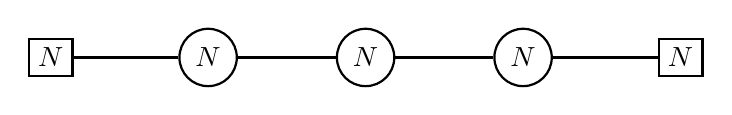
\begin{tikzpicture}[thick]
  \node[circle,draw] (one) at (0,0) {$N$};
  \node[circle,draw]  (two) at (2,0) {$N$};
  \node[circle,draw]  (three) at (4,0) {$N$};
  \node[rectangle,draw]  (flav1) at (-2,0) {$N$};
  \node[rectangle,draw]  (flav2) at (6,0) {$N$};
  \draw[-](one)--(two);
  \draw[-](two)--(three);
  \draw[-](one)--(flav1);
  \draw[-](flav2)--(three);
\end{tikzpicture}
\end{equation}
All the gauge couplings are exactly marginal since each gauge group has $2N$ flavours. The flavour symmetry of this theory is $\U(1)\times\U(1)\times\U(N)\times\U(N)$, where the $\U(1)$s come from the bifundamentals and the $\U(N)$s come from the fundamentals at the start and and of the quiver.\\
One can generate many more examples like this, for example
\begin{equation}
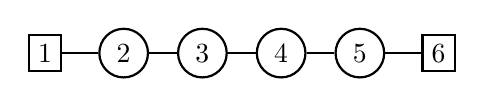
\begin{tikzpicture}[thick]
  \node[circle,draw] (one) at (0,0) {$2$};
  \node[circle,draw]  (two) at (1,0) {$3$};
  \node[circle,draw]  (three) at (2,0) {$4$};
  \node[circle,draw]  (four) at (3,0) {$5$};
  \node[rectangle,draw]  (flav1) at (-1,0) {$1$};
  \node[rectangle,draw]  (flav2) at (4,0) {$6$};
  \draw[-](one)--(two);
  \draw[-](two)--(three);
  \draw[-](three)--(four);
  \draw[-](one)--(flav1);
  \draw[-](flav2)--(four);
\end{tikzpicture}
\end{equation}
where, again, all the gauge couplings are marginal. One could ask why we do not branch around, but mathematically the shape of the graph is quite constrained by the requirement on the number of flavours. This is very similar to what happens with Dinkin diagrams in Lie algebras. The conformal quivers will always look like a sequence of gauge groups or that it bifurcates at the ends, or a loop (affine Dinkin diagrams). One can also get some exeptional diagrams.

One could also start to play with the gauge groups by looking at real groups: for $\USp(2N)$ we need $2N+2$ fundamentals so that the flavour group is $\SO(4N+4)$. The same can be said with an $\SO(2N)$ with $2N-2$ flavours. These allow to make quivers alternating $\USp$ and $\SO$ groups with half hypers connecting them. The continuous flavour symmetry will be just the one at the end of the quivers.

With a little bit of combinatorial work one can write down all the superconformal $\cN=2$ lagrangians with marginal couplings. What are the most general $\cN=2$ SCFT with gauge group $G=\SU(2)^{n}$? Let us write down some examples: 
\begin{enumerate}
	\item $\SU(2)$ with one adjoint is $\cN=4$ susy gauge theory. 
	\item $\SU(2)$ with $4$ fundamentals $N_{f}=4$, has $\SO(8)$ flavour symmetry.
\end{enumerate}
this is all with one gauge group. Let us go to two, beside trivial possibility of taking decoupled product of the last ones, 
\begin{equation}
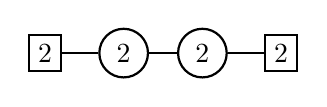
\begin{tikzpicture}[thick]
  \node[circle,draw] (one) at (0,0) {$2$};
  \node[circle,draw]  (two) at (1,0) {$2$};
  \node[rectangle,draw]  (flav1) at (-1,0) {$2$};
  \node[rectangle,draw]  (flav2) at (2,0) {$2$};
  \draw[-](one)--(two);
  \draw[-](one)--(flav1);
  \draw[-](flav2)--(two);
\end{tikzpicture}\qquad
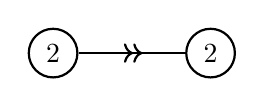
\begin{tikzpicture}[thick,decoration={
    markings,
    mark=at position 0.6 with {\arrow{>>}}}]
  \node[circle,draw] (one) at (0,0) {$2$};
  \node[circle,draw]  (two) at (2,0) {$2$};
  \draw[postaction={decorate}](one)--(two);
\end{tikzpicture}
\end{equation}
For the right one, one would think to have a $\U(2)$ flavour symmetry, but since the fundamental rep is pseudoreal, then the product of two fundamentals is real so we actually have a $\USp(4)$ flavour symmetry. The left one is more typical: there is a $\SO(4)^{2}$ coming from external fundamentals, while from the bifundamental there is a $\USp(2)$. But really the flavour group is $\SU(4)^{5}$ since $\SO(4)\sim\SU(2)\times\SU(2)$ and $\USp(2)\sim\SU(2)$.\\
Notice also that a pair of bifundamentals $(Q,\tilde Q)$ can be combined into one single $\hat Q$ which carries a $\USp(2)$ index
\begin{equation}
	\hat Q_{i_{1}i_{2}a}
\end{equation}
just writing $8=2\times2\times2$. These three indices play the same roles but the first two are gauged. But there is no reason to why I shouldn't be able to gauge other ones. We represent this object as a junction
\begin{equation}
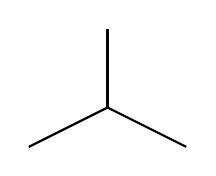
\begin{tikzpicture}[thick]
  \draw[-](0,0.5)--(0,-0.5);
  \draw[-](0,-0.5)--(-1,-1);
  \draw[-](0,-0.5)--(1,-1);
\end{tikzpicture}
\end{equation}
This adds two fundamental to every gauge group, but marginallity requires four fundamentals, and so we need two blocks, for example the $\SU(2)$ $N_{f}=4$ case is given by
\begin{equation}
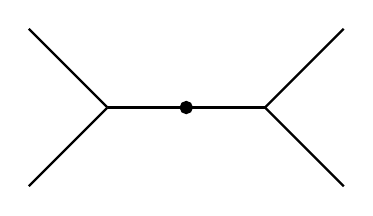
\begin{tikzpicture}[thick]
  \draw[-](0,0)--(1,-1);
  \draw[-](1,-1)--(0,-2);
  \draw[-](1,-1)--(2,-1);
  \draw[-](2,-1)--(3,-1);
  \draw[-](3,-1)--(4,0);
  \draw[-](3,-1)--(4,-2);
  \filldraw[black] (2,-1) circle (2pt) node[]{};
\end{tikzpicture}
\end{equation}
where the dot means the gauged group. We can also see, at least a subgroup, of the flabvour symmetry: in fact it is manifest an $\SU(2)^{4}\sim \SO(2)^{2}\subset \SO(8)$ flavour symmetry.

With this basic building block I can construct much more complicated theories. For any threevalent graph $\Gamma$ one gets a theory $T_{\Gamma}$ labelled by the graph. There are a couple of exeptional situations: take for example the following
\begin{equation}
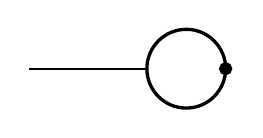
\begin{tikzpicture}[thick]
	\draw[-](0,0)--(1.5,0);
	\filldraw[color=black, fill=white, very thick](2,0) circle (0.5);
 	\filldraw[black] (2.5,0) circle (2pt) node[]{};
\end{tikzpicture}
\label{eq:N4}
\end{equation}
where two of the flavour symmetries are identified and gauged. What happens when we decompose $2\times 2\times 2a$? The first two give an adjoint plus a singlet that is not gauged. So this picture is $\SU(2)$ $\cN=$ plus a floating singlet. The singlet is important since now we can do 
\begin{equation}
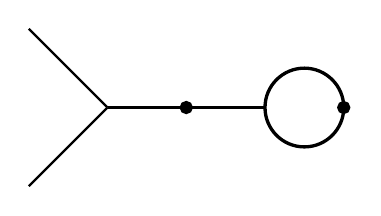
\begin{tikzpicture}[thick]
  \draw[-](0,0)--(1,-1);
  \draw[-](1,-1)--(0,-2);
  \draw[-](1,-1)--(2,-1);
  \draw[-](2,-1)--(3,-1);
  \filldraw[color=black, fill=white, very thick](3.5,-1) circle (0.5);
  \filldraw[black] (4,-1) circle (2pt) node[]{};
  \filldraw[black] (2,-1) circle (2pt) node[]{};
\end{tikzpicture}
\end{equation}
the adjoint, from the point of view of the central gauge group, looks like $3/2$ of a fundamental but with the singlet we have another $1/2$ fundamental that we can therefore gauge.

Let us discuss some of the properties of these theories $T_{\Gamma}$. Suppose to have $n$ external legs and $g$ loops. Without loops is very easy to count vertices and internal legs. Every loop removes two external legs and adds a vertex. Therefore we have $\SU(2)^{3g-3+n}$ gauge group. In particular there are going to be $3g-3+n$ gauge couplings $\tau_{i}$. There are also going to be $3g-3+n$ order parameters for the IR theory $\Tr\phi_{i}^{2}$ (coulomb branch order parameters).Notice that these order parameters and gauge couplings are intimately connected: if I want to change the gauge coupling I just take the lagrangian and add a prepotential term
\begin{equation}
	L+\delta\tau_{i}\int\dd[2]{\theta}\dd[4]{x}\Tr\phi^{2}_{i}
\end{equation}
There is also a flavour symmetry group $\SU(2)^{n}$, one for every external leg. In particular there are the mass parameters for this flavour group $\Tr M^{a}_{b}$. The mass parameter and the Coulomb branch scalars enter in the same way, so the mass parameters are just the order parameters for very weakly gauged flavour group.\\
For every $n,g$ the skeleton of the theory is the same, but they differ in how the matter couple.

\section{S-dualities}
We need to understand the S-dualities for these theories. We start from the simple cases. Consider $\cN=4$ $\SU(2)$ gauge theory. By moving in the Coulomb branch, the central charge $Z$ is uncorrected. The particles that move around in the Coulomb branch are: a W-boson (vector multiplet + hypermultiplet) which is half-BPS which has electric charge $1$ and magnetic charge $0$. At weak coupling it has a relatively small mass $Z=a$. Moving in the coulomb branch, we produce more particles. For example there is a magnetic monopole, half-BPS, and sit in the same multiplet as the $W$-boson but they have magnetic charge $1$ and electric charge $0$. It has a very heavy mass in the weak coupling limit $Z\sim \tau a$, but as $\tau\rightarrow 0$ they become lighter and lighter, becoming lighter than the $W$-boson. So in this limit, it does not make sense to think about the $W$-boson as the fundamental particle and as the monopole as some derived one. So we conjecture the existence of some sort of EM duality which exchanges them. The first test that this might be true, came out from looking at the full spectrum of magnetic monopoles and dyons. By quantizing one finds dyons $q_{M}=1$ and $q_{e}=n$. There are also magnetic monopoles with $q_{M}=2$ and dyons with $q_{e}=2n+1$. By going further one finds that there is a whole lattice of particles with electric and magnetic charges which are coprime $\gcd(q_{e},q_{m})=1$. By requiring that there is no wall crossing for half-BPS states, which means that the weakly coupled spectrum is actually the spectrum everywhere, we see that we have a spectrum of particles which is invariant under $\tau\rightarrow M\tau$ with $M\in \SL(2,\bbZ)$. This gives us a lot of weakly coupled regions which are divided by some strongly coupled regions.

One might wonder if the gauge coupling of the IR from which one can find the mass of the light fields, is the same parameter of the UV lagrangian. But this is an ill-defined question since the answer depends on the renormalization scheme. But we choose a renormalization scheme, when the masses are turned off, to have $\tau^{UV}=\tau^{IR}$.

Without wall crossing, we expect that the IR S-duality is still a symmetry in the UV since the spectrum of half-BPS states is the same.

Let us consider now the following theory $\SU(2)$ with $N_{f}=4$ flavours, which has $\SO(8)$ flavour symmetry. If the mass parameters, which sit in the cartan of $\SO(8)$, are turned off and if the vev of $\phi$ is zero, this theory has an exactly marginal gauge coupling $\tau$. By giving $\langle\Tr\phi^{2}\rangle=2a^{2}$ then, the central charge function cannot be corrected
\begin{equation}
	Z=(q_{e}+\tau^{IR}q_{m})a
\end{equation}
This theory seems to enjoy S-duality. But does the spectrum allow it? We have a $W$-boson ($q_{e}=2,q_{m}=0)$ plus a fundamental hypermultiplet which remember
\begin{equation}
	Q_{i}^{s}\tilde Q_{s}^{j}\phi^{i}_{j}
\end{equation}
becomes massless of mass $a$ and electric charge $1$. We have a flavour symmetry group which is unbroken so we label this particles by their $\SO(8)$ rep $\mathbf{8}_{v}$.\\
Surely there will be a classical solution in the Coulomb branch which is a smooth magnetic monopole solution with $q_{m}=1$ (quantizing it without flavour it is an hypermultiplet). With flavours there are more zero-modes: precisely there are $2N_{f}=8$ fermionic zero modes $\psi^{s}$ which transform in a vector of $\SO(8)$. What happens when we quantize them? We impose commutation relations
\begin{equation}
	\acomm{\psi^{s}}{\psi^{p}}=\delta^{sp}
\end{equation}
which tells us that these spinors are just gamma matrices that act on the monopoles: the monopole states live in spinor reps of the flavour group. Since the $\psi^{s}$ are also charged under the gauge group, they change the electric charge of the monopoles. The dyons
which have even electric charge sit in a positive chirality spinor and the ones with odd electric charge sit in a negative chirality spinor. There are also going to be particles with higher magnetic charges. Let us look just at the other ones for now.		
As $\tau\rightarrow\infty$ we are in the original weakly coupled limit, so we have a $W$-boson and hypermultiplet in $\mathbf{8}_{v,q_{e}}$. Then at $\tau=0$ we have monopoles in the spinor rep $\mathbf{8}_{s}$ while for $\tau=1$ we have ones in $\mathbf{8}_{c}$. This seems to be a problem but actually $\SO(8)$ has a $S_{3}$ outer automorphism group which exchanges these three representations\footnote{Symmetries of the Dynkin Diagram give rise to outer automorphisms of the Lie algebra. In the case where the Lie group is simply connected, such automorphisms are in one-to-one correspondance with group automorphisms. But when the Lie group is not simply connected all bets are off. Since $\pi_{1}(\SO(n))$ is of of order 2 (for $n>2$), some care must be taken. The second point is that the Dynkin Diagram of $\SO(8)$ actually has more symmetry, leading to the so called triality automorphism. This automorphism, in particular, maps $\text{Spin}(8)$, the universal covering, to itself and does not descend to $\SO(8)$.}. This is a good input by S-duality accompanied by the triality. In the fundamental region of the UHP we have three regions which are exchanged by the triality.

\subsection{Do the graph theory have S-dualities}
Let us start with the simplest theory $\SU(2)\times\SU(2)$

\begin{equation}
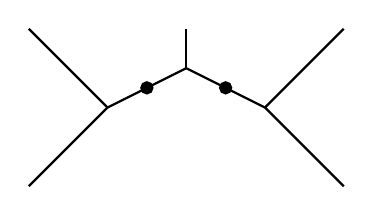
\begin{tikzpicture}[thick]
  \draw[-](0,0)--(1,-1);
  \draw[-](1,-1)--(0,-2);
  \draw[-](1,-1)--(2,-0.5);
  \draw[-](2,-0.5)--(2,0);
  \draw[-](2,-0.5)--(3,-1);
  \draw[-](3,-1)--(4,-2);
  \draw[-](3,-1)--(4,0);
  \filldraw[black] (1.5,-0.75) circle (2pt) node[]{};
  \filldraw[black] (2.5,-0.75) circle (2pt) node[]{};
\end{tikzpicture}
\end{equation}

All the fields are all fields with $3$ $\SU(2)$ indices some of which are gauge. The flavour symmetries are $\SO(4)\sim\SU(2)_{a}\times\SU(2)_{b}$ (from the left external legs) and an $\SU(2)_{c}$ (from the single internal leg) from the bifundamental and another $\SO(4)$ (from the other external legs). This theory hasd two exactly marginal gauge couplings $\tau_{1,2}$ and naively the parameter space should be the product of two upper half planes. I cannot go directly to IR but first explore the boundaries of this moduli space. I fix one gauge coupling to be very weak. In this region this theory just becomes $\SU(2)$ with $N_{f}=4$ with a very weakly gauged flavour symmetry group. This theory has three different lagrangian description. But if I want to see how this carries over to the original theory, I have to be careful to see what happens to the $\SU(2)$ flavour that I want to gauge and how the triality acts on it.\\
We have an $\SO(4)\times\SO(4)\subset\SO(8)$, therefore $\mathbf{8}_{v}=(\mathbf{4})\times(\mathbf{4})$. But the vector os $\SO(4)$ is just the product of the fundamental reps of the two $\SU(2)$ therefore becomes $(\mathbf{2}_{a}\times \mathbf{2}_{b})\times(\mathbf{2}_{c}\times \mathbf{2}_{2})$. Under triality, we excange $8_{v}$ with another $8_{s,c}$. The three cusps are just
\begin{equation}
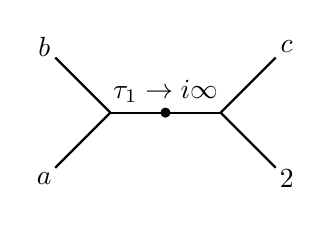
\begin{tikzpicture}[thick,scale=0.7]
  \node at (-.2,.2) {$b$};
  \node at (-.2,-2.2) {$a$};
  \node at (4.2,.2) {$c$};
  \node at (4.2,-2.2) {$2$};
  \draw[-](0,0)--(1,-1);
  \draw[-](1,-1)--(0,-2);
  \draw[-](1,-1)--(2,-1);
  \draw[-](2,-1)--(3,-1);
  \draw[-](3,-1)--(4,0);
  \draw[-](3,-1)--(4,-2);
  \filldraw[black] (2,-1) circle (2pt) node[above]{$\tau_{1}\rightarrow i \infty$};
\end{tikzpicture}\qquad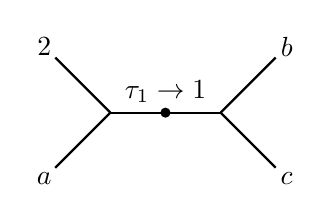
\begin{tikzpicture}[thick,scale=0.7]
  \node at (-.2,.2) {$2$};
  \node at (-.2,-2.2) {$a$};
  \node at (4.2,.2) {$b$};
  \node at (4.2,-2.2) {$c$};
  \draw[-](0,0)--(1,-1);
  \draw[-](1,-1)--(0,-2);
  \draw[-](1,-1)--(2,-1);
  \draw[-](2,-1)--(3,-1);
  \draw[-](3,-1)--(4,0);
  \draw[-](3,-1)--(4,-2);
  \filldraw[black] (2,-1) circle (2pt) node[above]{$\tau_{1}\rightarrow 1$};
\end{tikzpicture}\qquad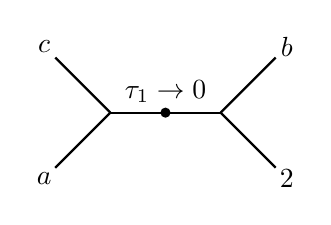
\begin{tikzpicture}[thick,scale=0.7]
  \node at (-.2,.2) {$c$};
  \node at (-.2,-2.2) {$a$};
  \node at (4.2,.2) {$b$};
  \node at (4.2,-2.2) {$2$};
  \draw[-](0,0)--(1,-1);
  \draw[-](1,-1)--(0,-2);
  \draw[-](1,-1)--(2,-1);
  \draw[-](2,-1)--(3,-1);
  \draw[-](3,-1)--(4,0);
  \draw[-](3,-1)--(4,-2);
  \filldraw[black] (2,-1) circle (2pt) node[above]{$\tau_{1}\rightarrow 0$};
\end{tikzpicture}
\end{equation}
which are exchanged by triality operation. So on the full theory, the triality acts as follows (where we can do the same job on the other coupling).

If the moduli space is really the product of two UHP we should be able to do S-duality on both nodes one after the other and viceversa and get the same result. 
\begin{figure}[H]
\includegraphics[width=\textwidth]{dualities.pdf}
\end{figure}
But what happens is that the two are not the same. But the two are related by S-duality. We found a pentagon of dualities. Here one gets a polytope made up of pentagons and triangles: the boundary of the parameter space (permutahedron, all the ways one can permute the $5$ flavour symmetries $5!/4$). So the hypotesis of the two UHP is wrong.

So what happens to a generic theory $T_{\Gamma}$? We have some trivalent graph and each S-duality operation reorganizes the four legs that come out of a segment. Through this basic operations we can relate all graphs with the same number of external leaves and loops (number of loops $g$ gives formula for dimension of Coulomb branch of the theory). There is a big moduli space $M_{g,n}$ (generalize notion of modular region?) of some $4d$ SCFT which with many cusps on the bundary each looking with some lagrangian description of $T_{\Gamma}$ with $g$ loops and $n$ leaves.\\
This $M_{g,n}$ has a bunch of charts in which I have a trivalent graph $\Gamma$ and a bunch of coordinates for each edge. Each chart looks like the upper region of the product of two UHP. But we want to combine all this charts together to glue the charts using S-dualities. This reminds us of Riemann surfaces. Instead of trying to build this $M_{g,n}$ by hand, I can see that there is a very famous moduli space with exactly the right dimension and properties. This is the space of complex structures of Riemann surfaces of genus $g$ with $n$ punctures. Let us see if we can really write charts which are naturally parametrized by the gauge couplings of my lagrangian.

Suppose to have a certain trivalent graph $\Gamma$. Associate to this graph a bunch of spheres with three marked points. We want to build out a Riemann surface of genus $g$ and $n$ punctures. There is a pretty natural way of doing it: every time I want to glue together two spheres to have a sensible Riemann surface which makes out my graph. What I can do is take some local coordinate system around this marked point and some local coordinates $z_{1}$ which goes to zero at the point. Take another one on the other sphere $z_{2}$ which goes together on the other marked point. To glue them together we declare that the following is satisfied
\begin{equation}
	z_{1}z_{2}=q
\end{equation}
where $q$ is some parameter. When $q=0$ we get the equation for two separate planes (so the two surfaces are disjoint and only touch at one point), with different $q$ they start merging together. So there is a certain patch in parameter space in the Riemann surface which has this coordinate system given by the $q_{i}$. To make sure is a good coordinate patch we should have $3g-3+n$ $q_{i}$s, and this number is the dimension of the moduli space of complex structures of the Riemann surface. As $q_{i}\rightarrow 0$ we get spheres which are connected together by very thin tubes.

We now claim that 
\begin{equation}
	q_{i}=e^{2\pi i\tau_{i}}
\end{equation}
so that the basic shift of the $\theta$ angle leaves the $q_{i}$ invariant. Now we need to see if it makes sense, especially for the S-duality transformation.

Take $\SU(2)$ with $N_{f}=4$. I can glue two spheres in two ways to get two patches in the moduli space of the theory
\begin{figure}[H]
\includegraphics[width=\textwidth]{su2.pdf}
\end{figure}
The Riemann surface that we make with this gluing is just a sphere with four punctures. Suppose to put the puctures at $0,1,\infty$ where we picked some global coordinates on the spheres $z,w$ (Riemann sphere is $\bbC$). The gluing is just 
\begin{equation}
	\frac{z}{w}=q
\end{equation}
In the $w$ plane we have points at $0,1,q,\infty$. We wanted our parameter space to look like a UHP a (moduli space of the torus). Is very easy to make a torus out of a four punctured sphere: write the equation $y^{2}=P(z)$ where $P(z)$ is some polynomial with zeros at that four points
\begin{equation}
	y^{2}=z(z-1)(z-q)
\end{equation}
This describes an elliptic curve, a torus. The torus has a certain modular parameter $\tau(q)$. When comparing the three possibilities for the three theories one finds
\begin{equation}
	q\rightarrow1-q^{\prime},\qquad q\rightarrow\frac{1}{q^{\prime\prime}}
\end{equation}
and converting them to statements in $\tau$ they become exactly $\SL(2,\bbZ)$ transformations. The three patches really coincide with the three possible theories.

With this picture we can describe easily the moduli space. For example the (\ref{eq:N4}) graph, beign $\cN=4$ SYM is identified by taking the three-punctured sphere and connecting together two punctures $1,\infty$. In the $\bbC$ plane this looks like taking an annulus and connecting together the boundaries to make a torus. The modular parameter of the torus is then exactly the marginal coupling of $\cN=4$ SYM.

Now one would like to know that, now that we know the boundaries of the moduli space, there is going to be no problem going in. Since complex geometry is very strict we would expect it to work. To do so one should build the Seiberg-Witten curves and check that they really behave properly on the parameters (the IR lagrangian at each point).

So take above each point the Coulomb branch of the theory and check that it is fiberd properly and that it transforms well under S-dualities. Moreover the dimension of the CB is $3g-3+n$ which happens to be exactly as the dimension of the parameter space. This is not a coincidence: if you want to change the gauge coupling, you just need to change the lagrangian by adding a prepotential term
\begin{equation}
	L+\delta\tau_{i}\int \Tr\phi_{i}^{2}
\end{equation}
the expectation value of which is a coordinate on the CB $u_{i}$. Viceversa, every dimension two operator could be added to the lagrangian to give a coupling. So coupling and dimension two operators are in one-to-one correspondence. More is pretty clear that $u_{i}\delta\tau_{i}$ should be a 1-form, so should transform as a 1-form and this tells us how the CBs in each patches should be glued together. It should be glued together the same way as the cotangent bundle of $M_{g}$, $T^{*}M_{g}$. So the CB should be fiberd the same way as the cotangent bundle.

There is a very cute way to describe the cotangent bundle to a Riemann surface. First of all we should get a good way to describe $\tau_{i}$. How do I change the $q$s? I cut and then glue together again: take a path $\gamma$ and cut along the path and I glue it back after acting with a vector field which acts in a neighborhood of $\gamma$. Local transformation
\begin{equation}
	\delta\tau_{i}v^{i}\pdv{}{z}
\end{equation}
Quadratic differentials with single poles are just deformations in the coulomb branch. If one includes mass parameters on the punctures, the differential should have a double pole on the puncture.
\chapter{\texorpdfstring{$2d/4d$ correspondance}{2d4d}}
This theory is relevant for the $2d-4d$ correspondence where a $6d$ theory is put on a product space $X_4\times C_2$ 
\begin{equation}
	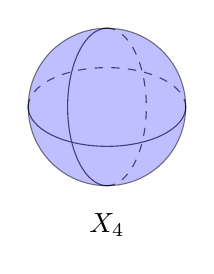
\begin{tikzpicture}[baseline={(0,0)}]
		\draw (-1,0) arc (180:360:1cm and 0.5cm);
    	\draw[dashed] (-1,0) arc (180:0:1cm and 0.5cm);
    	\draw (0,1) arc (90:270:0.5cm and 1cm);
    	\draw[dashed] (0,1) arc (90:-90:0.5cm and 1cm);
 		\filldraw[fill=blue!50, opacity=.5] (0,0) circle (1cm);

		\node at (0,-1.5) {$X_4$};
	\end{tikzpicture}\qquad\times\qquad
	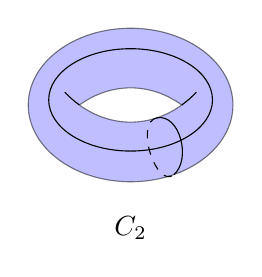
\begin{tikzpicture}[scale=1.3, baseline={(0,0)}]
		\draw[fill=blue!50,opacity=.5,even odd rule] (0,0) ellipse (1 and .75) 
		(-0.5,0) arc(120:60:1 and 1.25)  arc(-60:-120:1 and 1.25) coordinate[pos=0.25] (xt);
	   \draw (-0.5,0) arc(-120:-130:1 and 1.25) (0.5,0) arc(-60:-50:1 and 1.25);
	   \draw[] (-65:1 and .75) to[out=40,in=10] 
		node[pos=0.2,right]{} (xt);
	   \draw[dashed] (xt) to[out=-170,in=-140] (-65:1 and .75);
	   \draw[] (0.8,0.05) arc(0:360:0.8 and .5) {};
	   \node at (0,-1.2) {$C_2$};
	\end{tikzpicture}
\end{equation}
and compactified either on the first factor or on the second one. In the partition function of the $6d$ theory is a nice SUSY partition function that does not depende on the sizes of the two factors, then we expect the lower dimentional partition functions to match. Pictorially
\begin{equation*}
\begin{array}{rcl}
	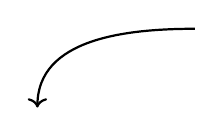
\begin{tikzpicture}[baseline={(0,0)}]
		\draw[->, thick] (0,0) to [out=180, in=90] (-2,-1);
	\end{tikzpicture}
	&\cZ_{S_{6d}}\left(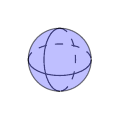
\begin{tikzpicture}[scale=.4,baseline={(0,-.1)}]
		\draw (-1,0) arc (180:360:1cm and 0.5cm);
    	\draw[dashed] (-1,0) arc (180:0:1cm and 0.5cm);
    	\draw (0,1) arc (90:270:0.5cm and 1cm);
    	\draw[dashed] (0,1) arc (90:-90:0.5cm and 1cm);
 		\filldraw[fill=blue!50, opacity=.5] (0,0) circle (1cm);
	\end{tikzpicture}\times
	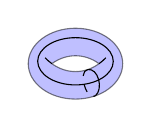
\begin{tikzpicture}[scale=.6, baseline={(0,-.1)}]
		\draw[fill=blue!50,opacity=.5,even odd rule] (0,0) ellipse (1 and .75) 
		(-0.5,0) arc(120:60:1 and 1.25)  arc(-60:-120:1 and 1.25) coordinate[pos=0.25] (xt);
	   \draw (-0.5,0) arc(-120:-130:1 and 1.25) (0.5,0) arc(-60:-50:1 and 1.25);
	   \draw[] (-65:1 and .75) to[out=40,in=10] 
		node[pos=0.2,right]{} (xt);
	   \draw[dashed] (xt) to[out=-170,in=-140] (-65:1 and .75);
	   \draw[] (0.8,0.05) arc(0:360:0.8 and .5) {};
	\end{tikzpicture}\right)&
	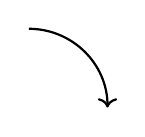
\begin{tikzpicture}[baseline={(0,0)}]
		\draw[thick, ->] (0,0) to [out=0, in=90] (1,-1);
	\end{tikzpicture}\\[15pt]
	%%%%%%%%%%%%%%%%%%%%%%%%%%%%%
	%%%%%%%%%%%%%%%%%%%%%%%%%%%%%
	\cZ_{S_{2d}\left[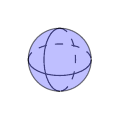
\begin{tikzpicture}[scale=.4,baseline={(0,0)}]
		\draw (-1,0) arc (180:360:1cm and 0.5cm);
		\draw[dashed] (-1,0) arc (180:0:1cm and 0.5cm);
		\draw (0,1) arc (90:270:0.5cm and 1cm);
		\draw[dashed] (0,1) arc (90:-90:0.5cm and 1cm);
		\filldraw[fill=blue!50, opacity=.5] (0,0) circle (1cm);
	\end{tikzpicture}\right]}\left(
	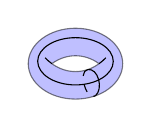
\begin{tikzpicture}[scale=.6, baseline={(0,0)}]
		\draw[fill=blue!50,opacity=.5,even odd rule] (0,0) ellipse (1 and .75) 
		(-0.5,0) arc(120:60:1 and 1.25)  arc(-60:-120:1 and 1.25) coordinate[pos=0.25] (xt);
		\draw (-0.5,0) arc(-120:-130:1 and 1.25) (0.5,0) arc(-60:-50:1 and 1.25);
		\draw[] (-65:1 and .75) to[out=40,in=10] 
		node[pos=0.2,right]{} (xt);
		\draw[dashed] (xt) to[out=-170,in=-140] (-65:1 and .75);
		\draw[] (0.8,0.05) arc(0:360:0.8 and .5) {};
	\end{tikzpicture}\right)
	&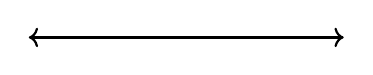
\begin{tikzpicture}[baseline={(0,0)}]
		\draw[thick,<->] (1,0) -- (5,0);
	\end{tikzpicture}&\cZ_{S_{4d}\left[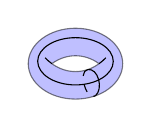
\begin{tikzpicture}[scale=.6, baseline={(0,0)}]
		\draw[fill=blue!50,opacity=.5,even odd rule] (0,0) ellipse (1 and .75) 
		(-0.5,0) arc(120:60:1 and 1.25)  arc(-60:-120:1 and 1.25) coordinate[pos=0.25] (xt);
		\draw (-0.5,0) arc(-120:-130:1 and 1.25) (0.5,0) arc(-60:-50:1 and 1.25);
		\draw[] (-65:1 and .75) to[out=40,in=10] 
		node[pos=0.2,right]{} (xt);
		\draw[dashed] (xt) to[out=-170,in=-140] (-65:1 and .75);
		\draw[] (0.8,0.05) arc(0:360:0.8 and .5) {};
	\end{tikzpicture}\right]}\left(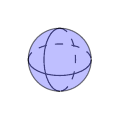
\begin{tikzpicture}[scale=.4,baseline={(0,0)}]
		\draw (-1,0) arc (180:360:1cm and 0.5cm);
		\draw[dashed] (-1,0) arc (180:0:1cm and 0.5cm);
		\draw (0,1) arc (90:270:0.5cm and 1cm);
		\draw[dashed] (0,1) arc (90:-90:0.5cm and 1cm);
		\filldraw[fill=blue!50, opacity=.5] (0,0) circle (1cm);
	\end{tikzpicture}\right)
\end{array}
\end{equation*}
These lower dimensional theories have been studied and loosely follow this classification
\begin{itemize}
	\item
		$S_{4d}\left[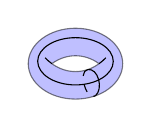
\begin{tikzpicture}[scale=.6, baseline={(0,-.1)}]
			\draw[fill=blue!50,opacity=.5,even odd rule] (0,0) ellipse (1 and .75) 
			(-0.5,0) arc(120:60:1 and 1.25)  arc(-60:-120:1 and 1.25) coordinate[pos=0.25] (xt);
			\draw (-0.5,0) arc(-120:-130:1 and 1.25) (0.5,0) arc(-60:-50:1 and 1.25);
			\draw[] (-65:1 and .75) to[out=40,in=10] 
			node[pos=0.2,right]{} (xt);
			\draw[dashed] (xt) to[out=-170,in=-140] (-65:1 and .75);
			\draw[] (0.8,0.05) arc(0:360:0.8 and .5) {};
		\end{tikzpicture}\right]$ : where $C_2$ is any Riemann surface with, possibly, punctures, are known class-S theories
	\item $S_{2d}\left[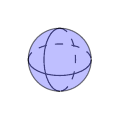
\begin{tikzpicture}[scale=.4,baseline={(0,-.1)}]
		\draw (-1,0) arc (180:360:1cm and 0.5cm);
		\draw[dashed] (-1,0) arc (180:0:1cm and 0.5cm);
		\draw (0,1) arc (90:270:0.5cm and 1cm);
		\draw[dashed] (0,1) arc (90:-90:0.5cm and 1cm);
		\filldraw[fill=blue!50, opacity=.5] (0,0) circle (1cm);
	\end{tikzpicture}\right]$: where $X_4=S^4$ is known as $2d$ Liouville-Toda theory
	\item $S_{2d}\left[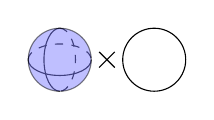
\begin{tikzpicture}[scale=.4,baseline={(0,-.1)}]
		\draw (-1,0) arc (180:360:1cm and 0.5cm);
		\draw[dashed] (-1,0) arc (180:0:1cm and 0.5cm);
		\draw (0,1) arc (90:270:0.5cm and 1cm);
		\draw[dashed] (0,1) arc (90:-90:0.5cm and 1cm);
		\filldraw[fill=blue!50, opacity=.5] (0,0) circle (1cm);
		\draw plot[mark=x,scale=5] coordinates{(0.30,0)};
		\draw (3,0) circle (1cm);
	\end{tikzpicture}\right]$: where $X_4=S^3\times S^1$ is known as $2d$ $q$-deformed YM
\end{itemize}
\section{\texorpdfstring{$2d$ Yang-Mills}{2dYM}}
In $2d$ there is no physical propagating degrees of freedom. Take $G$ to be a non-abelian Lie group. The action is of the form
\begin{equation}
	S\propto=\frac{1}{e^2}\int \dd[2]{x}\sqrt{\det g}\Tr F^2
\end{equation}
In $2d$ the only non-zero component of the curvature tensor is $F_{01}$ therefore
\begin{equation}
	\Tr F_{\mu\nu}F^{\mu\nu}=(g^{00}g^{11}-g^{01}g^{10})\Tr F_{01}^2=\det g^{-1}\Tr F_{01}^2
\end{equation}
so that 
\begin{equation}
	S \propto\frac{1}{e^2}\int\dd[2]{x}\sqrt{\det g}^{-1}\Tr F_{01}^2
\end{equation}
Therefore, the action only depends on the area of the surface, there is no additional dependence on the metric. This is a very special kind of $2d$ QFT. Whenever such a QFT is also a CFT, the theory is a $2d$ TQFT. The dependence on the coupling can be reabsorbed in the definition of the area.

We can solve this theory in many ways, but let us consider the Hamiltonian formalism putting the theory on cylinder. 
\begin{equation}
	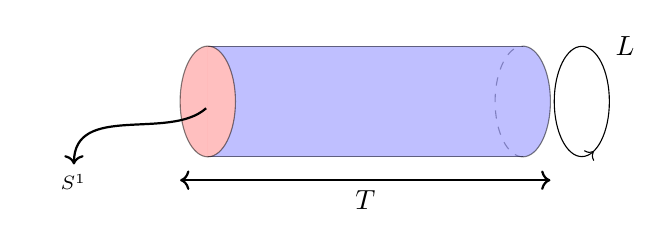
\begin{tikzpicture}[transform shape]
		\pic[
			tqft/cylinder, 
			rotate=90,
			fill=blue!50,
			scale=2,
			opacity=.5,
			cobordism edge/.style={draw},
			incoming upper boundary component 1/.style={draw, fill=red!50, opacity=.5},
			incoming lower boundary component 1/.style={draw, fill=red!50, opacity=.5},
			outgoing lower boundary component 1/.style={draw, dashed},
			outgoing upper boundary component 1/.style={draw},
			view from=incoming,
			at={(0,0)},
			every node/.style={transform shape},
			name=a
		];
		\draw[overlay,
				shift=(a-outgoing boundary), 
				xscale=.5,
				decoration={markings, mark=at position 0.8 with {\arrow{>}}}, 
				postaction={decorate}] {(1.5,0)} circle (.7) node[above left,yshift= 10pt, xshift=-15pt, thick] {};
		\draw[<->, thick, transform canvas={yshift=-1cm}] (a-incoming boundary.north) --node[below] {$T$}  (a-outgoing boundary.south) ;
		\node (L) at (5.3,0.7) {$L$};
		\draw[->, thick, transform canvas={xshift=.3cm,yshift=.2cm}] (a-incoming boundary) to [out=180,in=90] (-2,-1) node[below] {$\cH_{S^1}$};
	\end{tikzpicture}
\end{equation}\\

On $S^1$ we have an Hilbert space of states which, by taking the length of the circle to be $L$ can be defined as follows
\begin{equation}
	G\ni U=\text{Pexp}\int_0^L A_1 \dd x^1
\end{equation}
which is almost gauge invariant. At $0$ we still have a residual gauge transformation
\begin{equation}
	U\to gUg^-1
\end{equation}
So the Hilbert space is spanned by wavefunctions of $U$ which are invariant under the residual gauge transformation 
\begin{equation}
	\cH_{S^1}\ni \Psi(U)=\Psi(gUG^-1)
\end{equation}
One such basis for this Hilbert space is given by the characters of the representation $\chi_R(U)=\Tr_R U$ (class functions) which are indeed invariant under adjoint action. Moreover these are orthogonal given the following inner product
\begin{equation}
	\int \chi_R(U)\overline{\chi_{R^\prime}(U)}\dd{[U]}_{\text{Haar}}=\delta_{RR^\prime}
\end{equation}
Using the standard canonical quantization procedure, we can also find the Hamiltonian of the system. Being the only non-zero component of the curvature $F_{01}=E$, we have no magnetic field and therefore 
\begin{equation}
	H=\int_0^L\abs{E}^2\dd{x^1}=\int_0^L\frac{\delta}{\delta A_1(x_1)}\frac{\delta}{\delta A_1(x_1)}
\end{equation}
The action of the Hamiltonian on the basis is easily computed
\begin{equation}
\begin{split}
	H \chi_R(U) &= H \Tr_R\text{Pexp}\int_0^L T^a A_1^a\dd{x^1}\\
	&=\Tr_R\qty(\int_0^L T^a T^a) \dd{x^1}\Tr_R\text{Pexp}\int_0^L T^a A_1^a\dd{x^1}\\
	&=L c_2(R) \chi_R(U)
\end{split}
\end{equation}
which proves that the characters are indeed eigenstates of the hamiltonian. We can further idenfity the sides of the cylinder to get a torus $\bbT^2=S^1\times S^1$ and compute the partition function 
\begin{equation}
	Z_{2d}=\Tr_{\cH_{S^1}}e^{-HT}=\sum_R e^{-TL c_2(R)}
\end{equation}
which only depends on the area $TL$.

Next step, let us consider the following geometry: a disk with area $A$ (a cigar) 
\begin{equation}
	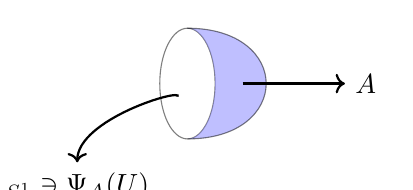
\begin{tikzpicture}[transform shape]
		\pic[
			tqft/cap,
			rotate=-90,
			scale=2,
			fill=blue!50,
			opacity=.5,
			cobordism edge/.style={draw},
			every outgoing boundary component/.style={draw},
			name=a
		];
		\draw[->, thick] (-3.3,0) -- (-2,0) node[right] {$A$};
		\draw[->, thick, transform canvas={yshift=-.6cm, xshift=-.4cm}] (a-outgoing boundary) to[in=90,out=90] (-5,-.4) node[below] {$\cH_{S^1}\ni\Psi_A(U)$};
	\end{tikzpicture}
\end{equation}\\
where now
\begin{equation}
	\cH_{S^1}\ni \Psi_A(U)
\end{equation}
which we like to determine (Hartle-Hawking wavefunction). To determine it we can consider joining a cylinder with area $A^\prime$ to the cigar and get\\

\begin{minipage}[c]{0.4\textwidth}
	\centering
		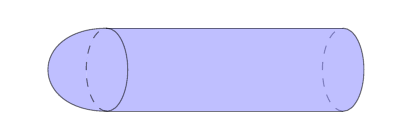
\begin{tikzpicture}[baseline={(0,-.2)}, transform shape]
			\pic[
				tqft/cap,
				scale=1.5,
				fill=blue!50,
				opacity=.5,
				cobordism edge/.style={draw},
				every outgoing boundary component/.style={fill=blue!50},
				name=h,
				rotate=90
			];
			\pic[
				tqft/cylinder, 
				fill=blue!50,
				scale=1.5,
				at=(h-outgoing boundary 1),
				opacity=.5,
				cobordism edge/.style={draw},
				incoming upper boundary component 1/.style={draw},
				incoming lower boundary component 1/.style={draw, dashed},
				outgoing lower boundary component 1/.style={draw, dashed},
				outgoing upper boundary component 1/.style={draw},
				view from=incoming,
				name=a,
				rotate=90
			];
		\end{tikzpicture}
	\end{minipage}
\begin{minipage}[c]{0.55\textwidth}
\begin{equation}
	\Psi_{A+A^\prime}(U)=e^{-A^\prime H}\Psi_A(U)
\end{equation}
\end{minipage}\\[10pt]
since we can easily change the area it is sufficient to know the zero area wavefunction. This can be understood from a path integral point of view. We have our spacetime to which there is cut out a zero-area disk. The holonomy around it needs to be one. Therefore the zero-area limit of this wavefunction must be a delta function. This is not square-integrable but we just add a constant
\begin{equation}
	\Psi_A(U)=\alpha\delta(U)=\sum_R f_R\chi_R(U)
\end{equation}
where the constants can be found as
\begin{equation}
	\alpha\chi_{R^\prime}(1)=f_{R^\prime}
\end{equation}
so that $f_R=\alpha \dim R$. Let us consider the pair of pants geometry with area $A$ so that we have three Hilbert spaces which should determine a vector in 
\begin{equation}
	\bigotimes_{i=1,2,3} H_{S^1}\ni \Psi_A(U_1,U_2,U_3)
\end{equation}
depending on the three holonomies.

By gluing a disk to one of the $S^1$ we get a cylinder with area $A+A^\prime$ to which we know the wavefunction. Therefore 
\begin{equation}
	\Psi_A(U_1,U_2,U_3)=\sum_R e^{-A c_2(R)}\frac{\chi_R(U_1)\chi_R(U_2)\chi_R(U_3)}{\dim R}
\end{equation}
We can now glue the three-punctured spheres in various ways to get many different geometries with different genus. For example, for genus $g=1$ with three punctures $n=3$ we can find 
\begin{equation}
	\frac{1}{\alpha^{2g-2+n}}\sum_R e^{-A c_2(R)}\frac{\prod_i \chi_R(U_i)}{(\dim R)^{2g-2+n}}
\end{equation}
Originally the constant $alpha$ came from the fact that the zero-area disk amplitude is a delta function which has to be normalized. On a genus $g$ surface, doing a QFT is very easy to generate a counterterm of the form 
\begin{equation}
	\delta S=\beta\int \dd[2]{x}\sqrt{g}R=\beta (2-2g)
\end{equation}
on a closed Riemann surface. This multiplies $Z$ by 
\begin{equation}
	e^{\beta(2-2g)}
\end{equation}
and the boundaries give some similar quantities depending on $n$. 

\section{$q$-deformed YM}
We consider the gauge group $G$ to be a standard Lie group. We deform it to a quantum group $G_q$ (the matrix entries become non-commutative). Take for example $\SU(2)_q$
\begin{equation}
	\begin{pmatrix}
		\alpha&\beta\\
		-\beta^*&\alpha^*
	\end{pmatrix},\qquad \alpha\beta=q\;\beta\alpha,\; \alpha\beta^*=q\;\beta^*\alpha,\ldots
\end{equation}
So we try to define a $2d$ YM in a lattice formulation for example, where all the link variables are replaced by a quantum group element instead of Lie group elements. This can be done in any dimensions but because of the non-commutativity one needs to define exacly in which order each link variable appears in the path integral. This is known at least in two dimensions how to do it consistently. In general dimensions is not known\dots

The end result is simple actually. Just replice the dimension of the rep by it's quantum dimension. When $G=\SU(N)_q$, then 
\begin{equation}
	\dim_q R = \chi_R\qty(\text{diag}(q^{\frac{N-1}{2}},q^{\frac{N-3}{2}},\cdots,q^{\frac{1-N}{2}})) 
\end{equation}
which in the limit $q\rightarrow1$ becomes $\chi_R(1)=\dim R$ as expected.

\section{Relation between Gaiotto theories and $q$-deformed YM}
Consider the superconformal index of $\cN=2$ $\SU(2)$ with $N_f=4$ flavours. This theory enjoys a special kind of S-duality discussed before. 

The relevant step in recongnizing the relationship between this theory and the $q$-deformed YM theory, is to consider the SCI of the Gaiotto theory in the limit of $q=t$. Consider in fact the half hypermultiplet contribution to the index 
\begin{equation}
	\Gamma(t^{1/2}z^\pm a^\pm b^\pm;p,q)\Gamma(t^{1/2}z^\pm c^\pm d^\pm;p,q)
\end{equation}
which explicitly, with $q=t$, gives
\begin{equation}
	\Gamma(t^{1/2}z^\pm;p,q)=\prod_{m,n\ge 0}\frac{1-z^{-1}p^{m+1}q^{n+\frac{1}{2}}}{1-zp^m q^{n+\frac{1}{2}}}\frac{1-z p^{m+1}q^{n+\frac{1}{2}}}{1-z^{-1}p^m q^{n+\frac{1}{2}}}
\end{equation}
There is a quasi complete cancellation between numerator and denominator such that the whole product just becomes
\begin{equation}
	\prod_{n\ge0}\frac{1}{1-q^{n+\frac{1}{2}}z}\frac{1}{1-q^{n+\frac{1}{2}}z^{-1}}
\end{equation}
and the dependence on $p$ vanished (this is a general behavior for $\cN=2$ SCFTs). This is due to the enanchement of SUSY in the aformentioned limit. 

So for the SCI of the original Gaiotto theory becomes 
\begin{equation}
	\frac{1}{2}\oint \frac{\dd z}{2\pi \I z}(1-z^2)(1-z^{-2})K(z)^{-2}\prod_{\pm\pm\pm}\prod_{n\ge 0}\frac{1}{1-q^{n+\frac{1}{2}}z^\pm a^\pm b^\pm}\frac{1}{1-q^{n+\frac{1}{2}}z^\pm c^\pm d^\pm}
\end{equation}
where
\begin{equation}
	K(z)^{-1}=\prod_{n\ge 0}(1-q^{n+1})\prod_\pm (1-q^{n+1}z^{\pm 2})
\end{equation}
The matter contribution can be rewritten with an infinite sum insted of an infinite product
\begin{equation}
	\prod_{\pm\pm\pm}\prod_{n\ge0}\frac{1}{1-q^{+\frac{1}{2}}z^\pm a^\pm b^\pm}=\frac{K(z)K(a)K(b)}{K_0}\sum_{n\ge 1}\frac{\chi_n(z)\chi_n(a)\chi_n(b)}{\chi_n(q^{\frac{1}{2}})}
\end{equation}
where
\begin{equation}
	\chi_n(a)=a^{n-1}+a^{n-3}+\cdots+a^{1-n}
\end{equation}
which is the character of 
\begin{equation}
	\begin{pmatrix}
		a&0\\
		0&a^{-1}
	\end{pmatrix}\in \SU(2)
\end{equation}
in the $n$-dimensional rep of $\SU(2)$, and
\begin{equation}
	K_0^{-1}=\prod_{n\ge0}(1-q^{2+n})
\end{equation}

We can plug this in the SCI formula and find
\begin{equation}
	\begin{split}
	\frac{1}{2}\oint &\frac{\dd{z}}{2\pi \I z}(1-z^2)(1-z^{-2})K(z)^{-2}\frac{K(z)K(a)K(b)}{K_0}\sum_{n\ge 1}\frac{\chi_n(z)\chi_n(a)\chi_n(b)}{\chi_n(q^{\frac{1}{2}})}\\
	&\times\frac{K(z)K(c)K(d)}{K_0}\sum_{m\ge 1}\frac{\chi_m(z)\chi_m(c)\chi_m(d)}{\chi_m(q^{\frac{1}{2}})}
	\end{split}
\end{equation}
The dependence on $z$ is localized now. Now $K(z)$ cancels out and the only $z$ dependent factors are in the charachers. There is a formula 
\begin{equation}
	\frac{1}{2}\oint \frac{\dd{z}}{2\pi \I z}(1-z^2)(1-z^{-2})\chi_m(z)\chi_n(z)=\delta_{m,n}
\end{equation}
since this is the orthogonal condition of the character on the torus of $\SU(2)$. Therefore the final result simplyfies a lot
\begin{equation}
	\frac{K(a)K(b)K(c)K(d)}{K_0^2}\sum_{n\ge 1}\frac{\chi_n(a)\chi_n(b)\chi_n(c)\chi_n(d)}{\chi_n(q^{\frac{1}{2}})^2}
\end{equation}
And now the invariance under the exchange of the various letters is manifest! But this is also just the partition function of $q$-deformed YM on a four punctured sphere with holonomies $a,b,c,d$ with the area sent to zero\\[10pt]
\begin{minipage}[c]{0.5\textwidth}
\centering
	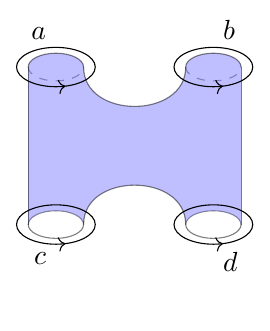
\begin{tikzpicture}[baseline={(0,0)}]
		\pic[
			tqft,
			incoming boundary components=2,
			outgoing boundary components=2,
			offset =0,
			fill =blue!50 ,
			opacity=.5,
			cobordism edge/.style={draw} ,
			incoming upper boundary component 1/.style={draw},
			incoming upper boundary component 2/.style={draw},
			incoming lower boundary component 1/.style={draw, dashed},
			incoming lower boundary component 2/.style={draw, dashed},
			every outgoing boundary component/.style={draw},
			name=a
			];
			\foreach \anchor/\x/\name/\shift in {incoming boundary 1/above left/a/+, incoming boundary 2/above right/b/+, outgoing boundary 1/below left/c/-, outgoing boundary 2/below right/d/-}
			\draw[overlay,
				shift=(a-\anchor), 
				yscale=.5,
				decoration={markings, mark=at position 0.8 with {\arrow{>}}}, 
				postaction={decorate}] {(0,0)} circle (.5) node[\x,yshift=\shift 1.5ex] {$\name$};
			\path (a-incoming boundary) +(0,.5) (a-outgoing boundary) +(0,-1);
	\end{tikzpicture}
\end{minipage}\hspace{-2cm}
\begin{minipage}[c]{0.5\textwidth}
	\begin{equation}
		\xlongrightarrow{A\rightarrow 0} \sum_R\frac{\chi_R(a)\chi_R(b)\chi_R(c)\chi_R(d)}{(\dim_q R)^2}\hspace{2cm}
	\end{equation}
\end{minipage}\\
This is the explicit $4d-2d$ correspondance! 

\section{\texorpdfstring{Connection to $6d$}{Mtheory}}
But why is this the case? The general idea is that each half-hypermultiplet corresponds to a three-punctured sphere and the gauge field is just a tube connecting punctures. 

The fact is that there is a certain $6d$ $\cN=(2,0)$ SCFT labelled by $G=ADE$\footnote{$A_n=\SU(n+1),D_n=\SO(2n),E_n=E_6,E_7,E_8$} such that its compactification on $S^1$ in the IR is given by a $5d$ $\cN=2$ SYM with gauge group $G$. By compactifying the $A_n$ case on the right punctured geometry the $4d$ theory is just the one studyied up to now.

But how do we know this? Starting from string theory, consider $N$ M5-branes on top of each other. The worldsheet theory is just the $6d$ $\cN=(2,0)$ gauge theory with gauge group $A_{N-1}$. For $D_N,E_N$ one can do similar constructions.

Before going to $4d$ $\cN=2$, we want to study $4d$ $\cN=4$ coming from a similar setup. Take the $6d$ SCFT and put it on $S^1$ with a radious $R_6$. The compactified theory is just $5d$ $cN=2$ SYM with $G$ gauge group 
\begin{equation}
	\int \dd[5]{x}\frac{1}{g^2_5}\tr F\wedge\star F+\cdots
\end{equation}
In $5d$ the inverse of the gauge coupling has dimension one since the kinetic term has dimension four. But the SCFT does not have any mass scale, therefore
\begin{equation}
	g_5^2\propto R_6
\end{equation}
Let us do another compactification on a circle with radius $R_5$. This becomes $4d$ $\cN=4$ SYM with gauge group G whose coupling constant is given by a usual Kaluza-Klein expansion
\begin{equation}
	\int \dd x_5\int\dd[4]x\frac{1}{g_5^2}\tr F\wedge \star F+\cdots
\end{equation}
where now the combination of $g_5^{-2}\dd{x_5}=g_{4}^{-2}$ and therefore 
\begin{equation}
	\frac{1}{g_4^2}\sim\frac{R_5}{R_6}
\end{equation}
Here we just put the $6d$ theory on a $T^2$ with sizes $R_6,R_5$ and got a $4d$ theory with $\tau=R_5 /R_6$. We could compactify in the other direction and get another $4d$ $\cN=4$ SYM with $\tau=R_6 / R_5$ which is just the inverse of the other one. This is the S-duality action which in this language is just Lorentz invariance in $6d$. 

In the $4d$ theory, basic excitations are point-like, but in $6d$ we have strings which can wrap the two cycles of the torus. These are tensionful strings, and therefore are massive excitations in the low energy theory. These have masses proportional to their tension and the radius of the two circles. The ratio of the mass of the excitations is just the complexified coupling. Recall that in $\cN=4$ the ratio of the mass of the W-boson and the monopole is given by the coupling $\tau$, so we can identify them with the wrapped strings. They come from the same object in $6d$. If one can write the lagrangian for this theory, S-duality would be completely trivial. But there perturbative excitations are going to be the same as semiclassical ones. This is very difficult.

\subsection{Kaluza-Klein reduction}
Consider a free massless scalar $\phi$ in $d$-dimensions and put it on $S^1$ of radius $R$. We can decompose the field in terms of the Fourier modes
\begin{equation}
	\phi(\vec{x},x_d)=\sum_n\phi_{(n)}(\vec{x})e^{in x_\frac{d}{R}}
\end{equation}
and the excitations are going to have massess of order 
\begin{equation}
	m=\abs{\frac{n}{R}}\quad\text{Kaluza-Klein tower}
\end{equation}
Consider $5d$ $\cN=2$ SYM with gauge group $G$ on flat space $\bbR^4\times \bbR$. This has instanton configurations which is point-like in $\bbR^4$ but it extends in time. It's a particle like excitation and the mass is given by the instanton action: if instanton number is $n$, the mass is 
\begin{equation}
	\frac{8\pi^2}{g_5^2}n\propto \frac{n}{R_6}
\end{equation}
So the mass of the instanton particle behave exactly like the KK tower. They are exactly the same when we fix the proportionality constant as
\begin{equation}
	g_{5d}^2=8\pi R_5^2
\end{equation}
So when we start from $6d$ part of the tower is included by the instanton configurations. There is an empirical fact: as far as BPS quantities are concerned, $5d$ SYM computations including instantons gives all the expected KK modes. In particular, if you add, say, KK towers of $5d$ YM fields, one gets double counting.

So if a lagrangian for this theory, it should have a gigantic gauge symmetry which would gauge away all this KK modes and identify them with the instantons. 

\subsection{Back to $6d$}
Now we can go to the $4d$ $\cN=2$ case. Take $6d$ $\cN=(2,0)$ of type $A_1=\SU(2)$\footnote{This does not mean that there is a $\SU(2)$ gauge field in $6d$.} and put it on a Riemann surface made of two $3$-punctured spheres glues on one puncture. Let us say that the tube has circumference length $R_6$ and length $R_5$. Use the fact that when we compactify the theory on a cicle, we get $5d$ $\cN=2$ SYM on a segment coupled to something at the ends. By compactifying again we get a $4d$ gauge multiplet with $\tau=R_5 / R_6$. But there is something going on on the ends, let us say there is a way to have a remaining $\cN=2$ instead of $\cN=4$ due to the boundary conditions. What is this boundary condition? From the $6d$ point of view we cannot say i for sure. But in $5d$ we see that the boundary is $\bbR^4$ so one can have some $4d$ theory with $\SU(2)$ flavour symmetry living on the boundary that couples to the bulk.The theory is exactly the trifundamental hypermultiplet $Q_{ABg}$. So let us try to determine what this $3$-punctured sphere is from $6d$: consider the SCI of the $4d$ theory obtained from $6d$ by putting the theory on this Riemann surface. Morally, the partition function of the $4d$ theory on $S^3\times S^1$ is just the partition function of the $6d$ theory on $S^3\times S^1\times \Sigma_g$. But since there is an $S^1$ we can compactify on it and get the partition function of the $5d$ SYM on $S^3\times \Sigma_g$. When compactifying again on $S^3$, computing the various corrections and including the KK modes around $S^3$ we get the partition function of a $2d$ theory on $\Sigma_g$ which is just $q$-deformed YM.

S-duality can be derived in a very nice way from $6d$. We found that the $6d$ theory on $\Sigma_4$ comprised of two $3$-punctured spheres connected by a cyclinder of circumference $R_6$ and length $R_5 $ gives rise to a $4d$ theory of two trifundamental hypermultiplet and an $\cN=2$ vector multiplet with coupling $\tau= R_5 / R_6$. We can make the coupling very small by having a very long cylinder. When we make the cylinder vert short, the theory is vert strongly coupled and when the two spheres are very near to each other we can split the $2d$ surgface in another way and consider the dimensional reduction along the other direction which just gives the S-dual theory.

\section{\texorpdfstring{Generalizing to $\SU(N)$}{SUN}}
We saw before that by compactifying $6d$ $\cN=(2,0)$ of type $A_1$ on a $3$-punctured sphere we obtain the theory of a free hypermultiplet. This is also confirmed by the structure of the SCI which was discussed and can be found from $6d$. The SCI is just given by 
\begin{equation}
	\frac{K(a)K(b)K(c)K(d)}{K_0^2}\sum_{n\ge 1}\frac{\chi_n(a)\chi_n(b)\chi_n(c)\chi_n(d)}{\chi_n(q^{\frac{1}{2}})^2}
\end{equation}
where 
\begin{equation}
	K(a)=1+\chi_\rm{adj}(a)q+\order{q^2},\qquad K_0=1+\order{q^2}
\end{equation}
If we expand the SCI up to order $q$ we get
\begin{equation}
	1+\frac{\chi_D(a)\chi_D(b)\chi_D(c)}{q^{\frac{1}{2}}+q^{-\frac{1}{2}}}+\order*{q}=1+q^{-\frac{1}{2}}\chi_D(a)\chi_D(b)\chi_D(c)+\order*{q}
\end{equation}
where the $q^{-\frac{1}{2}}$ signals the presence of a free hypermultiplet transforming in the flavour group representation $\chi_D(a)\chi_D(b)\chi_D(c)$, i.e. a trifundamental.

Generalizing to $\SU(N)$ 
\begin{equation}
	\frac{K(a)K(b)K(c)K(d)}{K_0^2}\sum_{n\ge 1}\frac{\chi_n(a)\chi_n(b)\chi_n(c)\chi_n(d)}{\chi_n(\operatorname{diag}(q^{\frac{N-1}{2}},q^{\frac{N-2}{2}},\ldots,q^{\frac{1-N}{2}}))}
\end{equation}
Consider $N=3$ with the expansion taken before 
\begin{equation}
	1+q\qty(\chi_\rm{adj}(a)+\chi_\rm{adj}(b)+\chi_\rm{adj}(c))+\frac{\chi_\rm{fund}(a)\chi_\rm{fund}(b)\chi_\rm{fund}(c)+\rm{antifund}}{q^-1+1+q^2}
\end{equation}
This seems like $E_6$ symmetry, in fact $\SU(3)_A\times\SU(3)_B\times\SU(3)_C\subset E_6$ where 
\begin{equation}
	78=8_A\oplus 8_B\oplus 8_C\oplus(3_A\otimes 3_B\otimes 3_C)\oplus (\bar{3}_A\otimes\bar{3}_B\otimes\bar{3}_C)
\end{equation}
This theory is known as the $E_6$ theory of Minahan-Nemeschansky. With this we can construct the duality between two copies of the $E_6 \times E_6$ theory (one factor from each $3$-punctured sphere).

More than this, being an $\SU(3)$ $\cN=2$ with $N_f=4$, we would like to understand the case of $\SU(3)$ with $N_f=6$. Before getting here we consider the case for general $N$. The theory is named $T_N$ and the duality works as expected. We do not really know what this $T_N$ theories actually are, but we know a lot about them; they are also non-lagrangian. Before diving into the lagrangian case of $\SU(N)$ with $N_f=2N$, let us discuss some geometric things. 

\subsection{Partial closure of punctures}
In general, given an $\cN=2$ SCFT $\cT$ with flavour symmetry $G_F$ it will have current operators. Thanks to susy we will have also fermion and scalar operators associated with the current 
\begin{equation}
	\mu_{(ij)}^a,\ \lambda_{\alpha i}^a, \ J^a_\mu
\end{equation}
where $i$ is an $\SU(2)_R$ index and $\mu$ is a $G_F$ adjoint scalar. In the language of class-S a puncture is a flavour symmetry. E.g. consider a bifundamental hypermultiplet $Q_a^i,\Tilde{Q}_i^a$ with $a,i=1,\ldots N$ and flavour is $\U(N)\times \U(N)$. Then there should be three scalar operators
\begin{equation}
	\mu^+=Q_a^i\Tilde{Q}^b_i,\quad \mu^-=(Q^\dagger)^a_i(\Tilde{Q}^\dagger)^i_a,\quad \mu^0=(Q^\dagger)^a_i Q^i_b-\Tilde{Q}^a_i(\Tilde{Q}^\dagger)^i_b
\end{equation}
where $\mu^+$ is a chiral field, $\mu^-$ is an anti-chiral and $\mu^0$ is just a D-term.


\backmatter
\phantomsection
\addcontentsline{toc}{chapter}{References}
\bibliography{reps}

\end{document}
